\documentclass[aspectratio=169]{beamer}
\usepackage{adjustbox}
\usepackage[utf8]{inputenc}
\usepackage{tikz}
\usepackage{hyperref}
\usepackage{multimedia}
\usepackage{ulem}
\usepackage{wasysym}
\usepackage{wrapfig}
\usetikzlibrary{mindmap,trees}

\usepackage{pbox}

\usepackage[absolute,overlay]{textpos}

% \usetikzlibrary{mindmap,trees}

\usepackage{smartdiagram}
\usetikzlibrary{shapes.geometric,calc}
\usetikzlibrary{shapes.symbols}
\usetikzlibrary{shapes.symbols,positioning}
\usepackage{metalogo}

\usetikzlibrary{backgrounds, calc, shadows, shadows.blur}

\newcommand\addcurlyshadow[2][]{
    % #1: Optional aditional tikz options
    % #2: Name of the node to "decorate"
    \begin{pgfonlayer}{background}
        \path[blur shadow={shadow xshift=0pt, shadow yshift=0pt, shadow blur steps=6}, #1]
        ($(#2.north west)+(.3ex,-.5ex)$)
        -- ($(#2.south west)+(.5ex,-.7ex)$)
        .. controls ($(#2.south)!.3!(#2.south west)$) .. (#2.south)
        .. controls ($(#2.south)!.3!(#2.south east)$) .. ($(#2.south east)+(-.5ex,-.7ex)$)
        -- ($(#2.north east)+(-.3ex, -.5ex)$)
        -- cycle;
   \end{pgfonlayer}
}


%%%%%%%%%%%%%%%%%%%%%%%%%%%%%%%%%%%%%%%%%%%%%%%%%%%%%%%%%%%%%%%%%%%
% Style modifications
%%%%%%%%%%%%%%%%%%%%%%%%%%%%%%%%%%%%%%%%%%%%%%%%%%%%%%%%%%%%%%%%%%%

\usetheme{Berlin}

%%% Fonts %%%

% Change font. Fontspec requires xelatex instead of pdflatex!
% Font catalog: https://www.tug.dk/FontCatalogue/
\usepackage{fontspec}

%\setsansfont{Comfortaa}
%\setsansfont{DejaVu Sans}
%\setsansfont{Fira Sans}

% Use "Fira Sans Light" as the normal font and the "Fira Sans" for
% bold fonts

\setsansfont[
  ItalicFont={Fira Sans Light Italic},
  BoldFont={Fira Sans},
  BoldItalicFont={Fira Sans Italic}]{Fira Sans Light}

\setbeamerfont{title}{size=\Large, series=\bfseries}
\setbeamerfont{frametitle}{size=\large, series=\bfseries}

%%% Slide template %%%

\setbeamertemplate{frames}[default]

% Empty headline / footline
\setbeamertemplate{headline}{}
\setbeamertemplate{footline}{}

% Remove navigation icons
\setbeamertemplate{navigation symbols}{}

%%% Colors %%%

\usecolortheme{crane}

\definecolor{lightgray}{RGB}{220,220,220}
\definecolor{darkgray}{RGB}{45,45,45}
%\definecolor{darkblue}{RGB}{0,86,137}
%\definecolor{darkblue}{RGB}{22,90,151}
\definecolor{lightblue}{RGB}{229, 245, 255}

%\definecolor{darkblue}{RGB}{1,1,100}


% Use the slide background in block environments                                                                                                      
\setbeamercolor{title}{fg=white,bg=darkgray}
\setbeamertemplate{blocks}[default]
\setbeamercolor{block title}{bg=}
\setbeamercolor{block body}{bg=lightgray}
\setbeamercolor{frametitle}{fg=white,bg=darkgray}
\setbeamerfont{block body}{size=\large}
\setbeamercolor{itemize item}{fg=black}
\setbeamertemplate{itemize items}[circle]
\setbeamercolor{section number projected}{bg=darkgray,fg=white}
\setbeamercolor{section in toc}{fg=black}
\setbeamercolor{subsection in toc}{fg=darkgray}

\addtobeamertemplate{block begin}{\pgfsetfillopacity{0.8}}{\pgfsetfillopacity{1}}
\addtobeamertemplate{frametitle}{\pgfsetfillopacity{1.0}}{\pgfsetfillopacity{1}}
\addtobeamertemplate{title page}{\pgfsetfillopacity{1.0}}{\pgfsetfillopacity{1}}

% Command to place the test (e.g. citation) in the center of the footer
\newcommand{\setfootercentertext}[1]{
  \setbeamertemplate{footline}{
    \hspace*{\fill}
    \raisebox{3mm}[0mm][0mm]{
      \tiny{#1}}\hspace*{\fill}}
}



\addtobeamertemplate{navigation symbols}{}{%
    \usebeamerfont{footline}%
    \usebeamercolor[fg]{footline}%
    \hspace{1em}%
    \insertframenumber/\inserttotalframenumber
}


%%%%%%%%%%%%%%%%%%%%%%%%%%%%%%%%%%%%%%%%%%%%%%%%%%%%%%%%%%%%%%%%%%%
% Content
%%%%%%%%%%%%%%%%%%%%%%%%%%%%%%%%%%%%%%%%%%%%%%%%%%%%%%%%%%%%%%%%%%%

%------------------------------------------------------------------------------
\title{Eine Einführung in das Maschinelle Lernen}
%------------------------------------------------------------------------------

\author{\small Konrad U. Förstner}

\institute{ZB MED -- Informationszentrum Lebenswissenschaften \& TH Köln}

\date{\scriptsize 
  Zertifikatskurs Data Librarian -- Module 3\\\ \\
  2002-02-10\\\ \\
  \href{https://creativecommons.org/licenses/by/4.0/}{
\includegraphics[width=0.88cm]{images/creative_commons_attribute.png}}
}

\logo{
  
\includegraphics[height=1.0cm]{images/ZBMED_2017_EN.pdf}
  
\includegraphics[height=0.8cm]{images/logo_TH-Koeln_CMYK_22pt.eps}
}

\begin{document}

%\setbeamertemplate{background}{
  % \includegraphics[height=\paperheight]{images/flickr_normanbleventhalmapcenter_2710796662_mod.jpg}
%}

\begin{frame}{}
  \titlepage
\end{frame}

\logo{}


\setcounter{tocdepth}{1}
\begin{frame}{}
   \tableofcontents
\end{frame}

%%%%%%%%%%%%%%%%%%%
\section{Einführung}
%%%%%%%%%%%%%%%%%%%

\begin{frame}
  % \frametitle{Basic concept of supervised machine learning}
  \begin{block}{}
    \vspace{0.5cm}
    \ \ \ \
    \begin{minipage}{0.10\textwidth}
      \begin{center}
        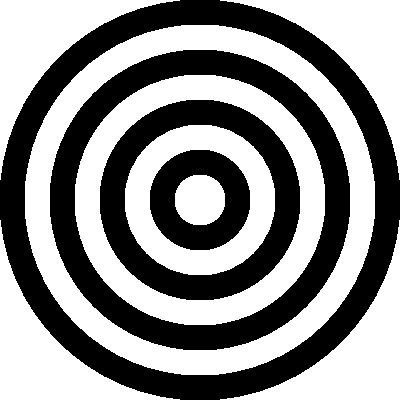
\includegraphics[width=1.6cm]{images/publicdomainvectors_target-plain.pdf}
      \end{center}        
    \end{minipage}
    \hfill
    \begin{minipage}{0.80\textwidth}
      After the lecture you should have a basic understanding of
      supervised machine learning approaches and potential
      applications in research.\\

      After the practical part you should be able to implement them
      with Python and the package scikit-learn.\\

      We will not cover the mathematical background. This is not
      needed at this level but recommended later.
    \end{minipage}
    \vspace{0.3cm}
  \end{block}
\end{frame}

\begin{frame}{}
   \tableofcontents[currentsection]
\end{frame}

% https://unsplash.com/photos/U3sOwViXhkY

\setbeamertemplate{background}{
  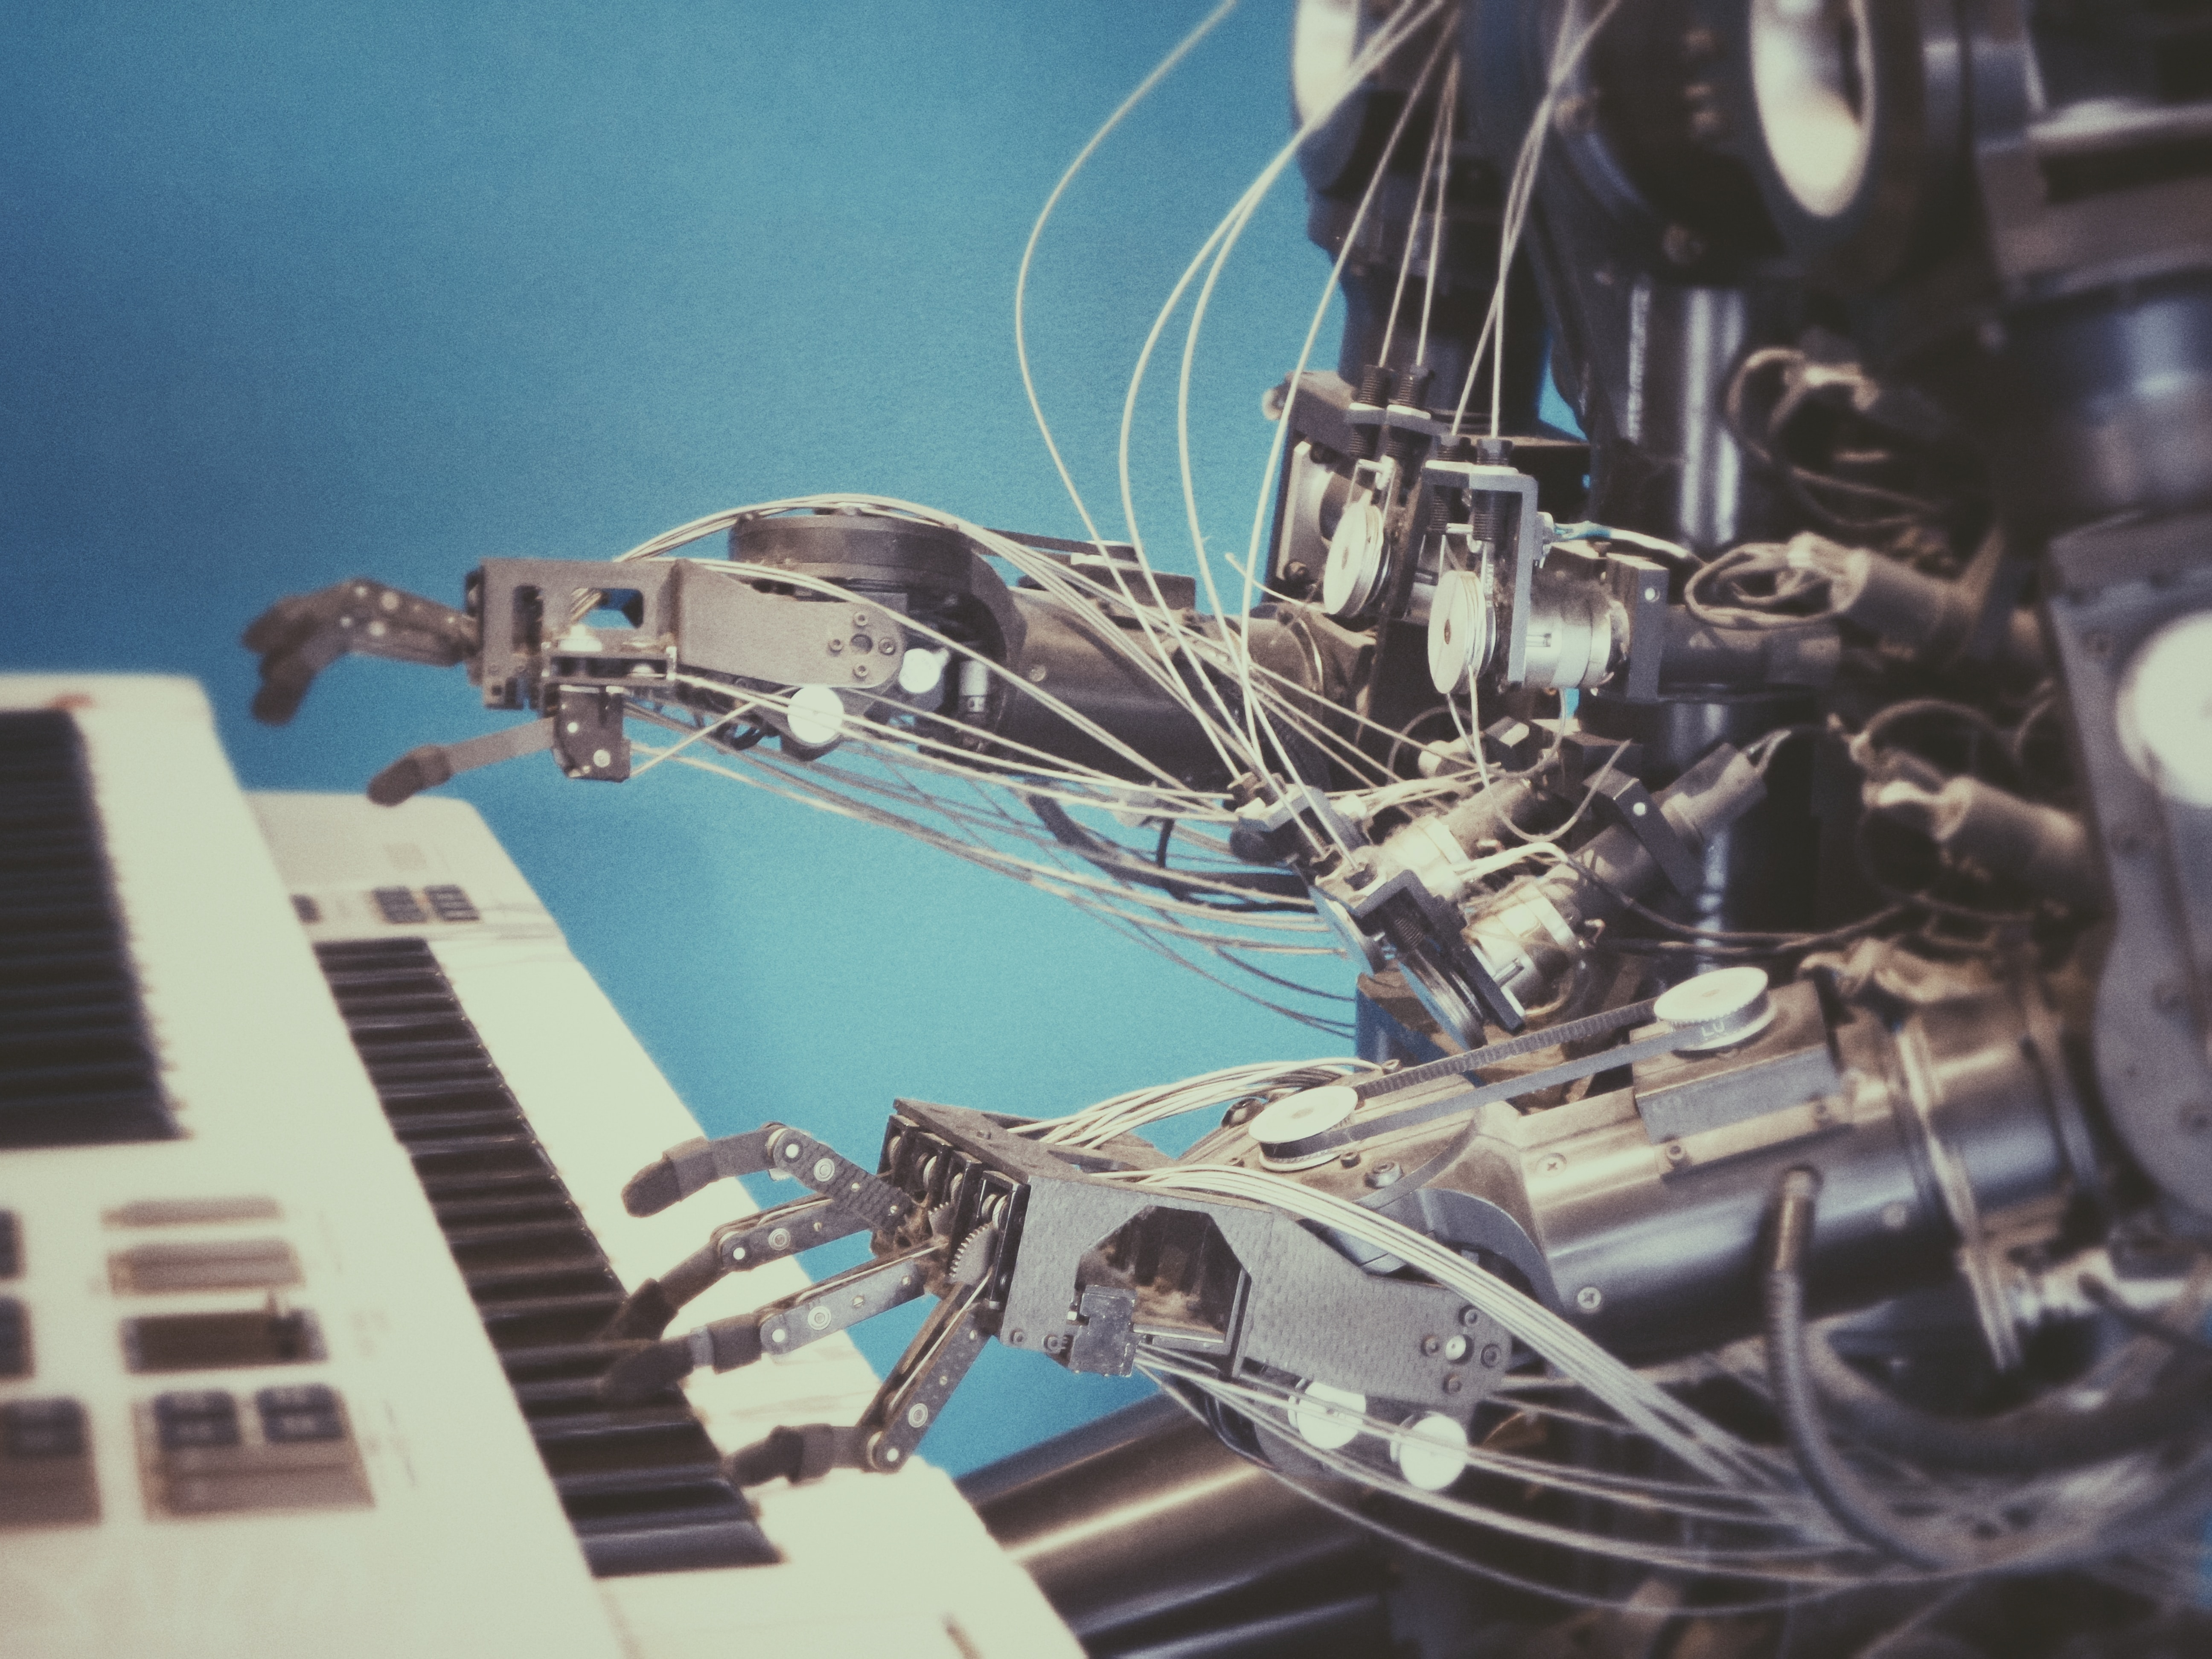
\includegraphics[width=\paperwidth]{images/robot_piano_franck-v-U3sOwViXhkY-unsplash.jpg}}
\setfootercentertext{
  \href{https://unsplash.com/photos/U3sOwViXhkY}{https://unsplash.com/photos/U3sOwViXhkY} -- CC0}
\begin{frame}
  \frametitle{}
\end{frame}
\setbeamertemplate{background}{}
\setfootercentertext{}

\begin{frame}
  \frametitle{}
  \begin{center}
    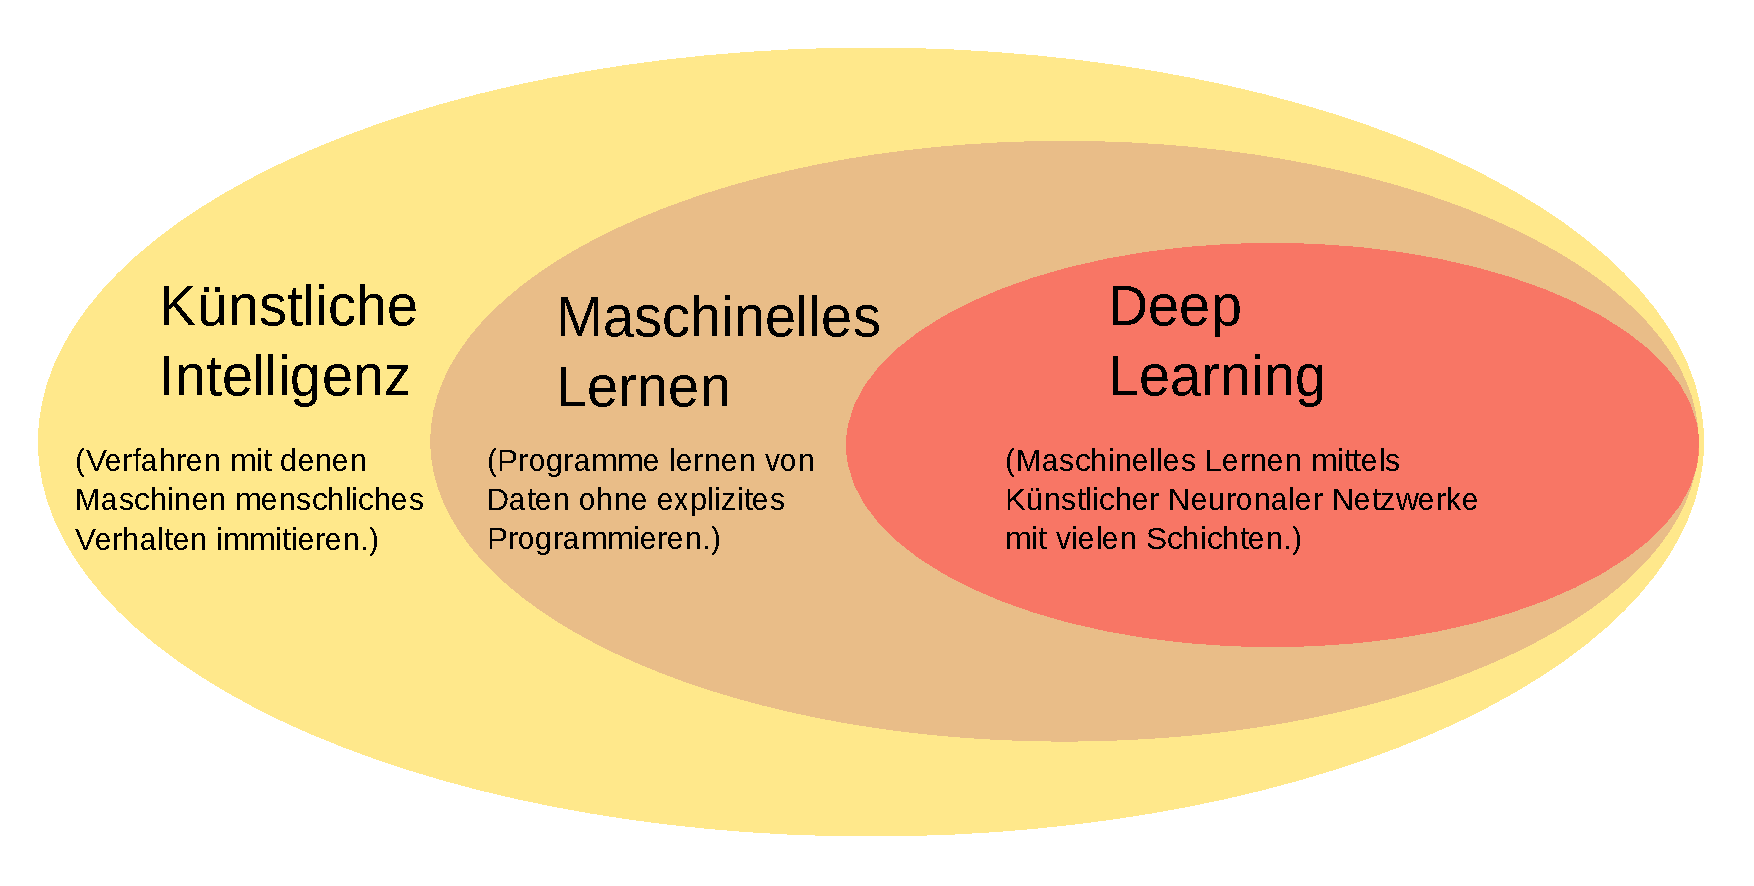
\includegraphics[width=13cm]{images/AI_Maschinelles_Lernen_Deep_Learning.pdf}
  \end{center}
\end{frame}

\begin{frame}

  \begin{center}
    \begin{adjustbox}{max totalsize={.9\textwidth}{.7\textheight},center}
    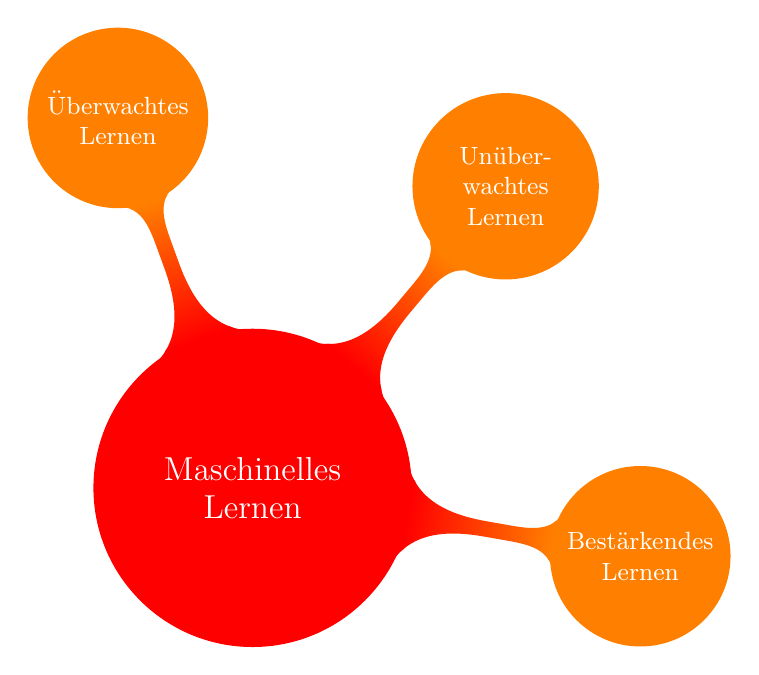
\begin{tikzpicture}
      \path[mindmap,concept color=red,text=white]
      node[concept] {Maschinelles\\Lernen}
      [clockwise from=110]
      
      child[concept color=orange] { node[concept] {Überwachtes Lernen}}
      child[concept color=orange] { node[concept] {Unüber-wachtes Lernen}}
      child[concept color=orange] { node[concept] {Bestärkendes Lernen}}

      ;
    \end{tikzpicture}  
    \end{adjustbox}
  \end{center}
\end{frame}

% Daten
% Hardware (GPUs)
% Algotthmen


\begin{frame}
  \frametitle{Anwendungsbeispiele}
  \begin{block}{}
    \begin{center}
      \begin{itemize}
      \item Text-Klassifikation wie Spam-Filter oder automatische
        Verschlagwortung von Artikeln
      \item Bilderanalyse - Erkennung von Objekten in Bilder
      \item Spracherkennung
      \item Recommender Systeme ("Kunden, die X gekauft haben, habe
        auch Y gekauft.")
      \item Deepfakes -- Synthetische Medien (Fotos, Videos)
      \end{itemize}
    \end{center}
  \end{block}
\end{frame}

%%%%%%%%%%%%%%%%%%%%%%%%%%%%%%%
\section{Entitäten und ihre Eigenschaften}
%%%%%%%%%%%%%%%%%%%%%%%%%%%%%%%

\begin{frame}{}
   \tableofcontents[currentsection]
\end{frame}

\begin{frame}
  \frametitle{Entitäten und ihre Eigenschaften}
  \begin{block}{}
    \begin{center}
      \textbf{Entitäten} (auch Datenpunkte genannt) werden durch ihre\\
      \textbf{Eigenschaften} beschrieben (auch Attribute, Merkmale
      oder Features genannte) die bestimmte
      \textbf{Eigenschaftenswerte} besitzen.
    \end{center}
  \end{block}    
\end{frame}

\begin{frame}
  \frametitle{Typisierung von Eigenschaften}
  \begin{block}{}
    \begin{itemize}
    \item kategorial
      \begin{itemize}
      \item nominal (z.B. Augenfarbe, Geschlecht)
      \item ordinal (z.B. sehr schlecht $<$ schlecht $<$ mittel $<$ gut $<$ sehr gut)
      \end{itemize}
    \item nummerisch
      \begin{itemize}
      \item diskrete (z.B. Anzahl an Buchseiten)
      \item kontinuiertlich (z.B. Regallänge)  
      \end{itemize}
    \end{itemize}
  \end{block}
\end{frame}


\begin{frame}
  \frametitle{Beispiel -- ein Buch}
  \begin{block}{}
    \begin{itemize}
    \item 456 Ausleihungen
    \item Buchrücken ist 4,2 cm breit
    \item Themenbereich "Biologie"
    \item als "lesenswert" bewertet
    \end{itemize}
  \end{block}    
\end{frame}

\begin{frame}
  \frametitle{Beispiel -- ein Buch}
  \begin{block}{}
    \begin{itemize}
    \item 456 Ausleihungen -- diskret nummerisch
    \item Buchrücken ist 4,2 cm breit -- nummerisch kontinuiertlich      
    \item Themenbereich "Biologie"  -- kategorial nominal
    \item als "lesenswert" bewertet -- kategorial ordinal
    \end{itemize}
  \end{block}        
\end{frame}

\begin{frame}
  \frametitle{}
  \begin{block}{}
    \begin{minipage}{0.15\textwidth}
      \ \ \
      
\includegraphics[width=1.6cm]{images/kuf_icons_warning_triangle.pdf}
    \end{minipage}
    \hfill
    \begin{minipage}{0.8\textwidth}
       Meistens muss man die Eigenschaften erst bearbeiten\\ bevor man
       damit man diese nutzen.
    \end{minipage}
  \end{block}
\end{frame}

\begin{frame}
  \frametitle{Feature (Subset) Selection}
  \begin{block}{}
    \begin{center}
      Auswahl von aussagekräftigen Eigenschaften
    \end{center}  
  \end{block}
\end{frame}  

\begin{frame}
  \frametitle{Feature Encoding}
  \begin{block}{}
    \begin{center}
      Übersetzen von kategorialen Eigenschaften in nummerische
    \end{center}
  \end{block}
\end{frame}

\begin{frame}
  \frametitle{Feature Encoding -- Beispiel}
  \begin{block}{}
    \vspace{0.5cm}
    \hspace{1cm}
    \begin{minipage}{0.3\textwidth}
      {\small
        \begin{tabular}{ll}
          \textbf{Buch ID} & \textbf{Kategorie}\\
          \hline
          000A & Biologie \\
          000B & Chemie \\
          000C & Biologie \\
          000D & Physik \\
          000E & Physik \\
        \end{tabular}
      }
    \end{minipage}
    \begin{minipage}{0.1\textwidth}
      $\Rightarrow$
    \end{minipage}
    \begin{minipage}{0.4\textwidth}
      {\small
        \begin{tabular}{llll}
          \textbf{Buch ID} & \textbf{Biologie} & \textbf{Chemie} & \textbf{Physik}\\
          \hline
          000A & 1 & 0 & 1\\
          000B & 0 & 1 & 0\\
          000C & 1 & 0 & 0\\
          000D & 0 & 0 & 1\\
          000E & 0 & 0 & 1\\
        \end{tabular}
      }
    \end{minipage}
    \hspace{1cm}
  \end{block}
\end{frame}  

\begin{frame}
  \frametitle{Feature Scaling}
  \begin{block}{}
    \begin{center}
      Normalisierug (z.B. auf Maximalwert oder Standardabweichung) von
      Werten um gleiche Gewichtung zu gewährleisten.
    \end{center}  
  \end{block}
\end{frame}

\begin{frame}
  \frametitle{Feature Scaling -- Beispiel}
  \begin{block}{}  
    \vspace{0.5cm}
    %\hspace{1cm}
    \begin{minipage}{0.43\textwidth}
      {\small
        \begin{tabular}{lll}
          \textbf{Buch ID} & \textbf{Breite [cm]} & \textbf{Gewicht [g]}\\
          \hline
          000A & 4.3 & 537\\
          000B & 5.3 & 703\\
          000C & 2.2 & 510\\
          000D & 1.5 & 200\\
          000E & 5.2 & 760\\
        \end{tabular}
      }
    \end{minipage}
    \begin{minipage}{0.08\textwidth}
      $\Rightarrow$
    \end{minipage}        
    \begin{minipage}{0.40\textwidth}
      {\small
        \begin{tabular}{lrr}
          \textbf{Buch ID} & \textbf{norm. Breite} & \textbf{norm. Gewicht}\\
          \hline
          000A & 0.81 & 0.70\\
          000B & 1.00 &  0.93\\
          000C & 0.42 & 0.67\\
          000D & 0.28 & 0.26\\
          000E & 0.98 & 1.00 \\
        \end{tabular}
      }
    \end{minipage}
    \hspace{1cm}
  \end{block}
\end{frame}

%%%%%%%%%%%%%%%%%%%
\section{Überwachtes Lernen (Supervised Learning)}
%%%%%%%%%%%%%%%%%%%

\begin{frame}{}
   \tableofcontents[currentsection]
\end{frame}


%-------------------------------
\subsection{Einführung Überwachtes Lernen}
%-------------------------------

\setcounter{tocdepth}{2}
\begin{frame}{}
   \tableofcontents[ 
     currentsubsection, 
     hideothersubsections,
     subsectionstyle=show/shaded]
\end{frame}

\begin{frame}
  \frametitle{Mit überwachten Lernen können zwei Problemklassen bearbeitet werden}
  \begin{center}
    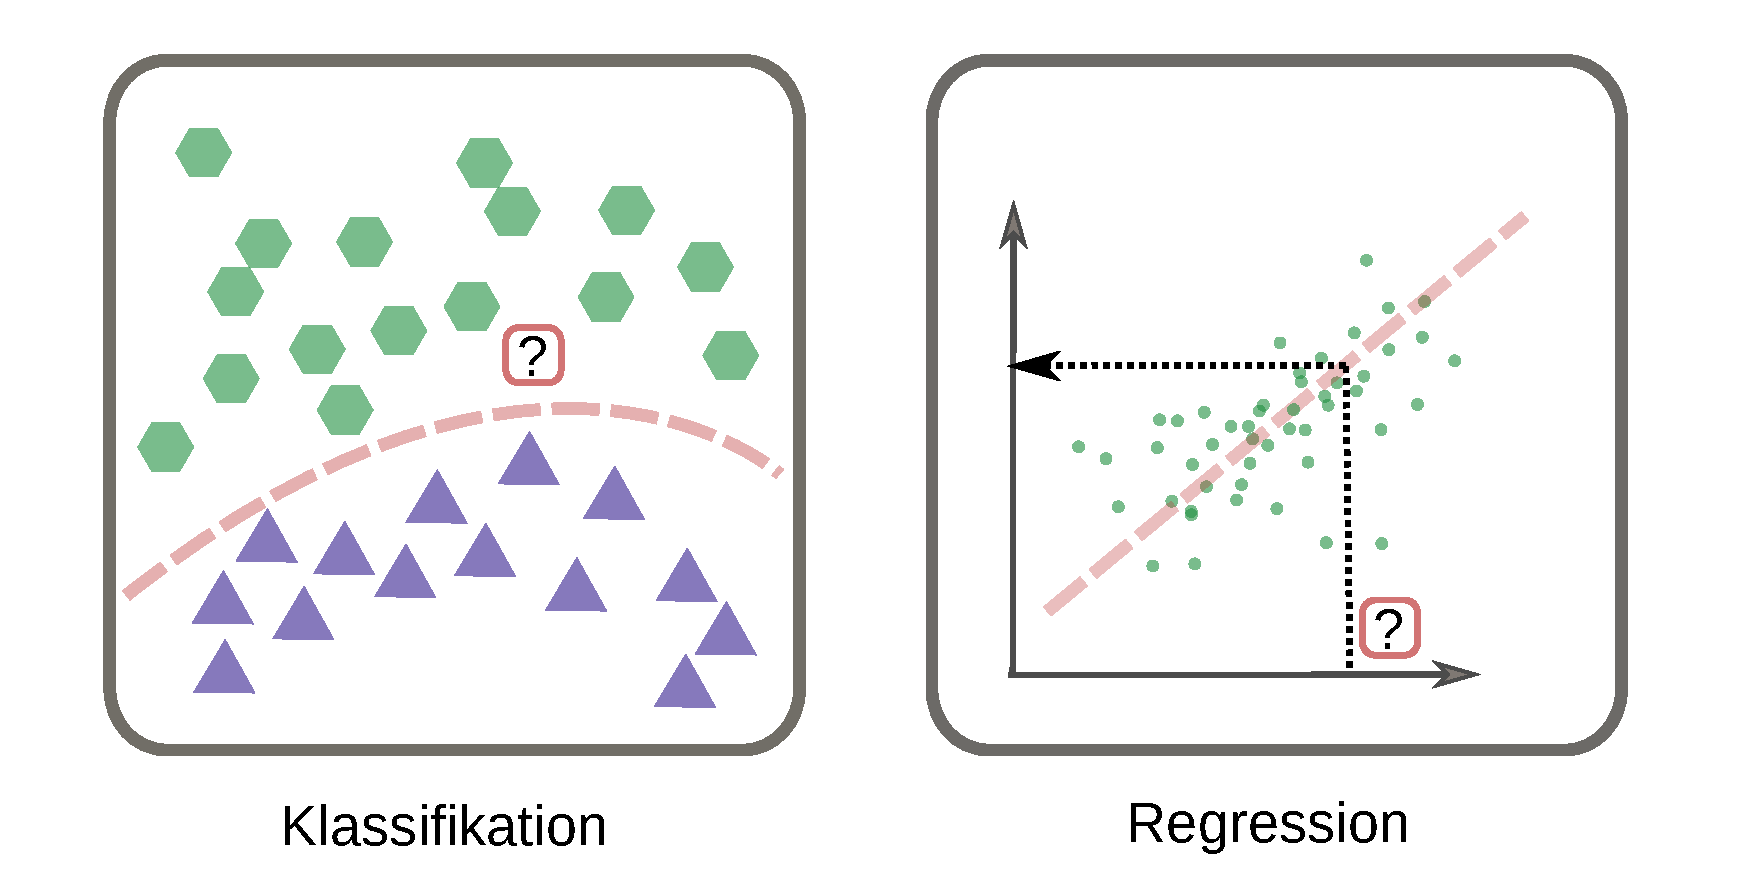
\includegraphics[width=13cm]{images/Klassifikation_and_Regression.pdf}
  \end{center}
\end{frame}

\begin{frame}
  \frametitle{Klassifikationstype}
  \begin{center}
    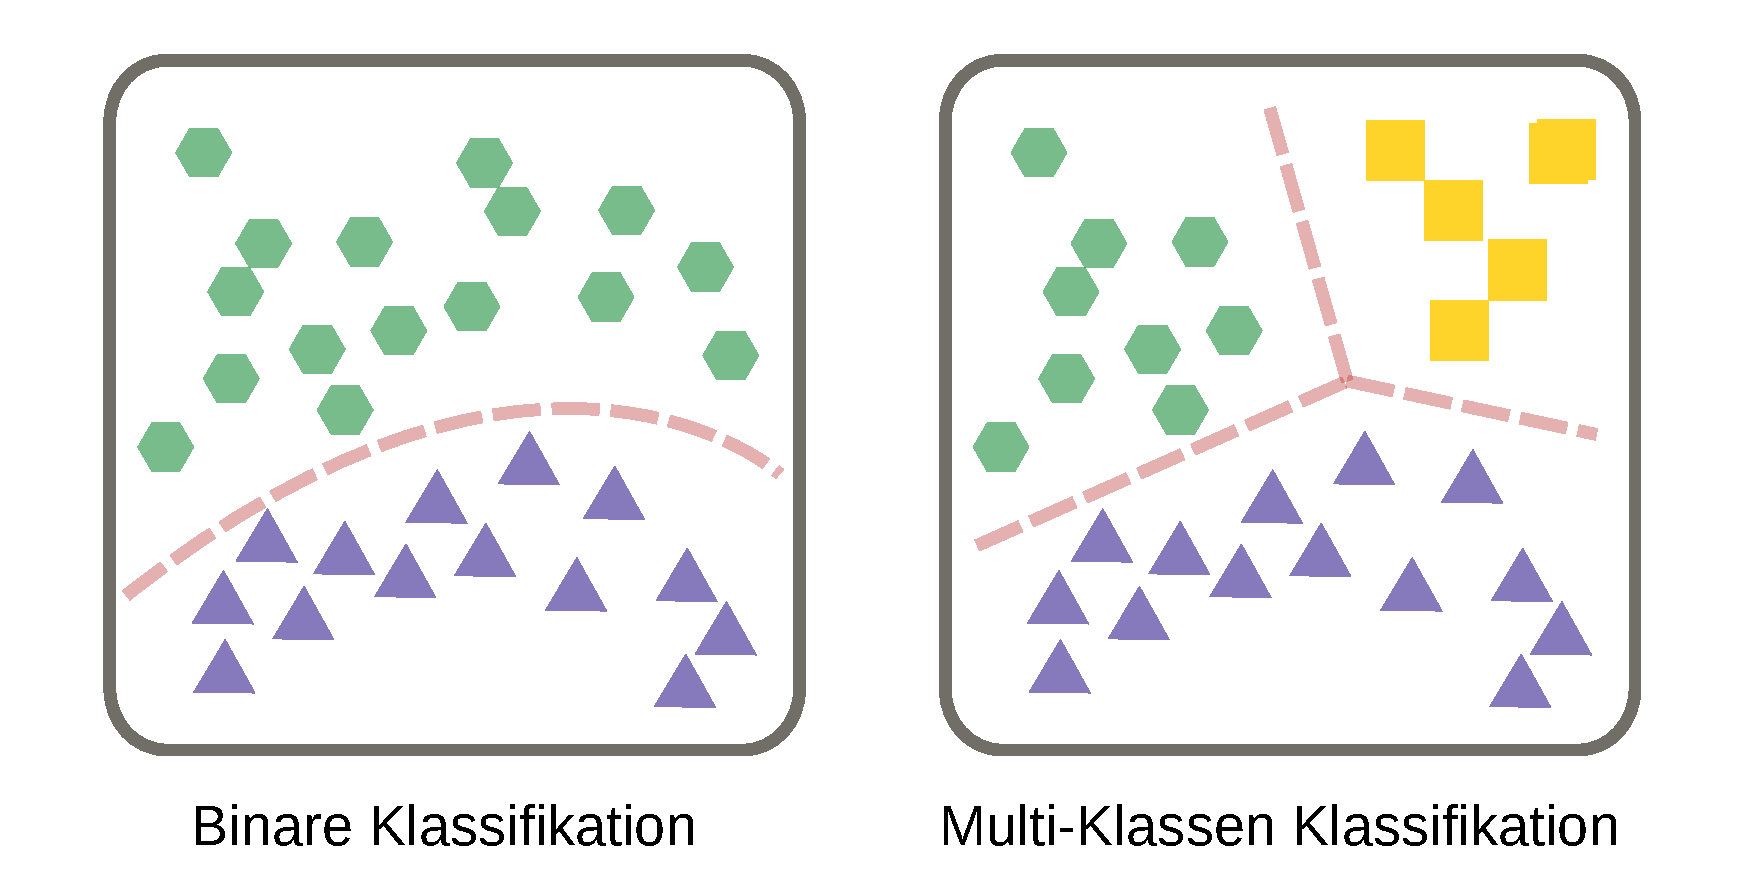
\includegraphics[width=13cm]{images/binary_vs_multi-class_classification.pdf}
  \end{center}  
\end{frame}

\begin{frame}
  \frametitle{Grudlegendes Konzept von überwachten Lernen}
  \begin{block}{}
    \vspace{0.5cm}
    \ \ \ \
    \begin{minipage}{0.15\textwidth}
      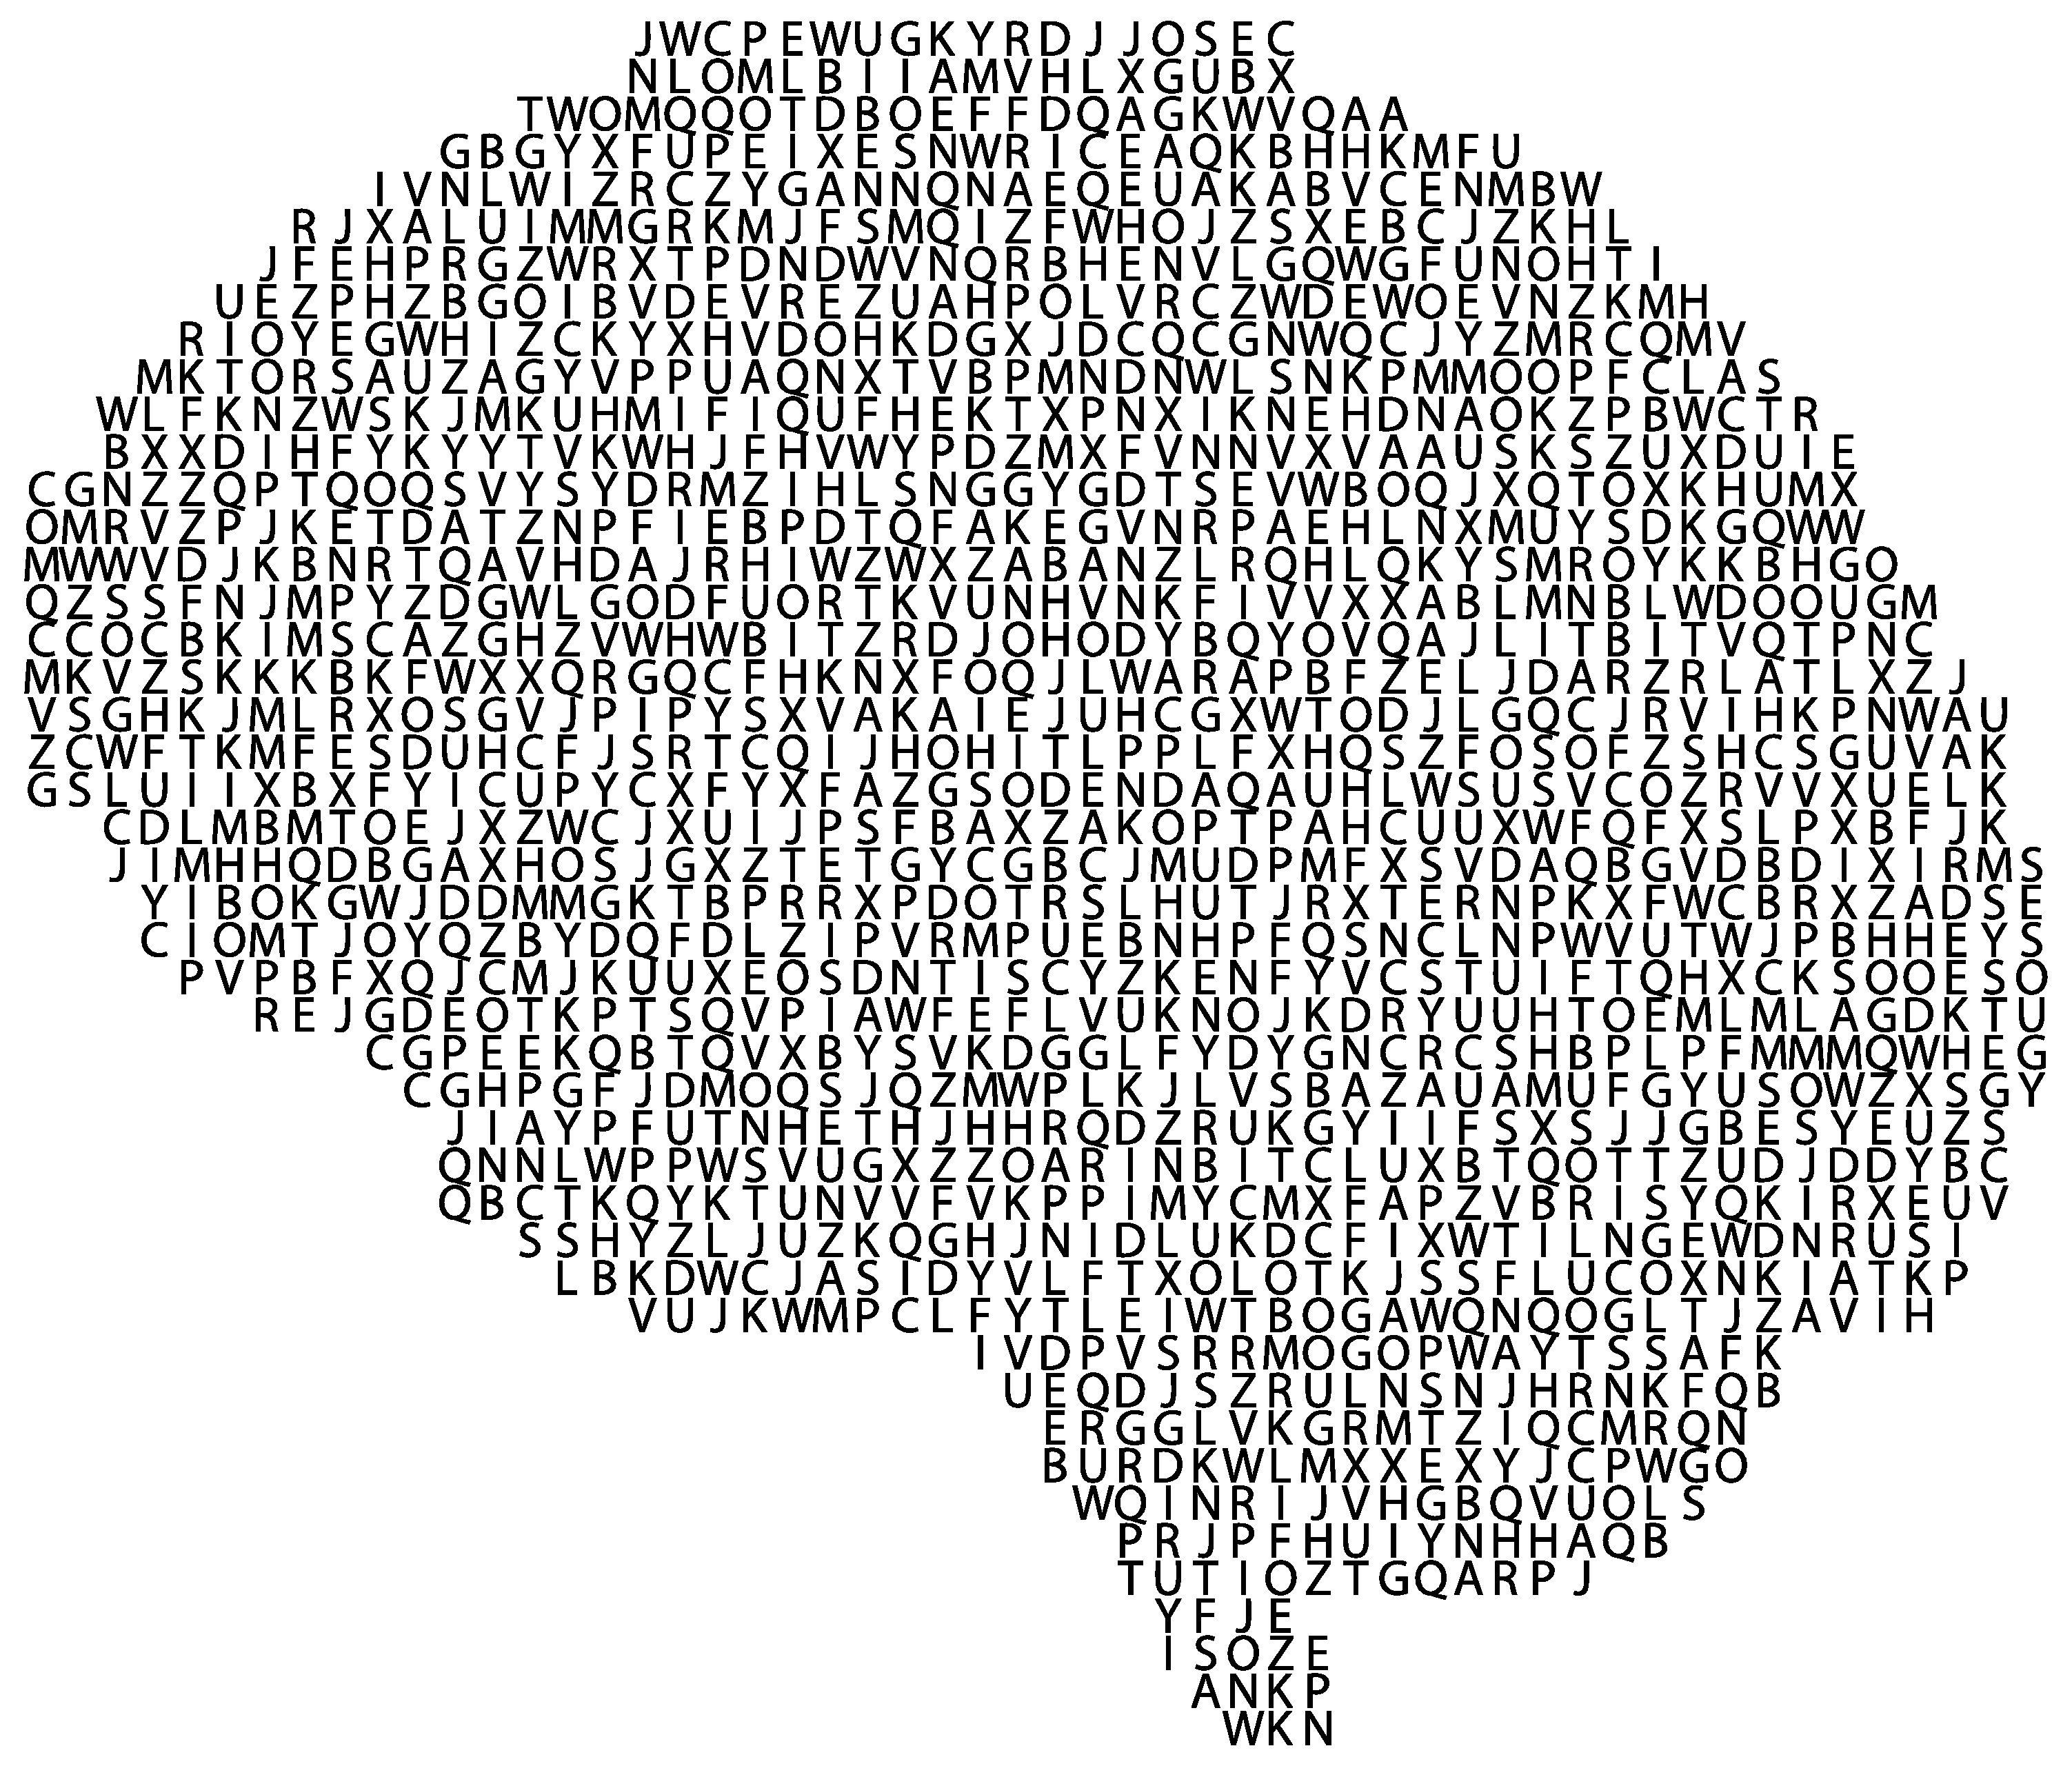
\includegraphics[width=1.6cm]{images/publicdomainvectors_Random-Alphabet-Brain.pdf}
    \end{minipage}
    \hfill
    \begin{minipage}{0.75\textwidth}
      Überwachtes Lernen heißt basierend von Beispielen\\
      generelle Modelle zu erzeugen.\\
    \end{minipage}
    \vspace{0.3cm}
  \end{block}
\end{frame}

\begin{frame}
  \frametitle{Grudlegendes Konzept von überwachten Lernen}
  \begin{block}{}
      \begin{center}
        Die erzgeugten Modelle mappen von einer zweidimentionalen
        Eingangmatrix-Matrix $X$ auf einen Ausgabe-Vektor $y$.

      $X_{1} \rightarrow y_{1}$\\
      $X_{2} \rightarrow y_{2}$\\
      $X_{3} \rightarrow y_{3}$\\
        \ \\
     Bei Klassifikation ist y ein Label, bei Regression ein nummerischer Wert.
      \end{center}
    \end{block}
\end{frame}


\begin{frame}
  \frametitle{Grudlegendes Konzept von überwachten Lernen}
  \begin{block}{}
    \vspace{0.5cm}
    \ \ \ \
    \begin{minipage}{0.15\textwidth}
      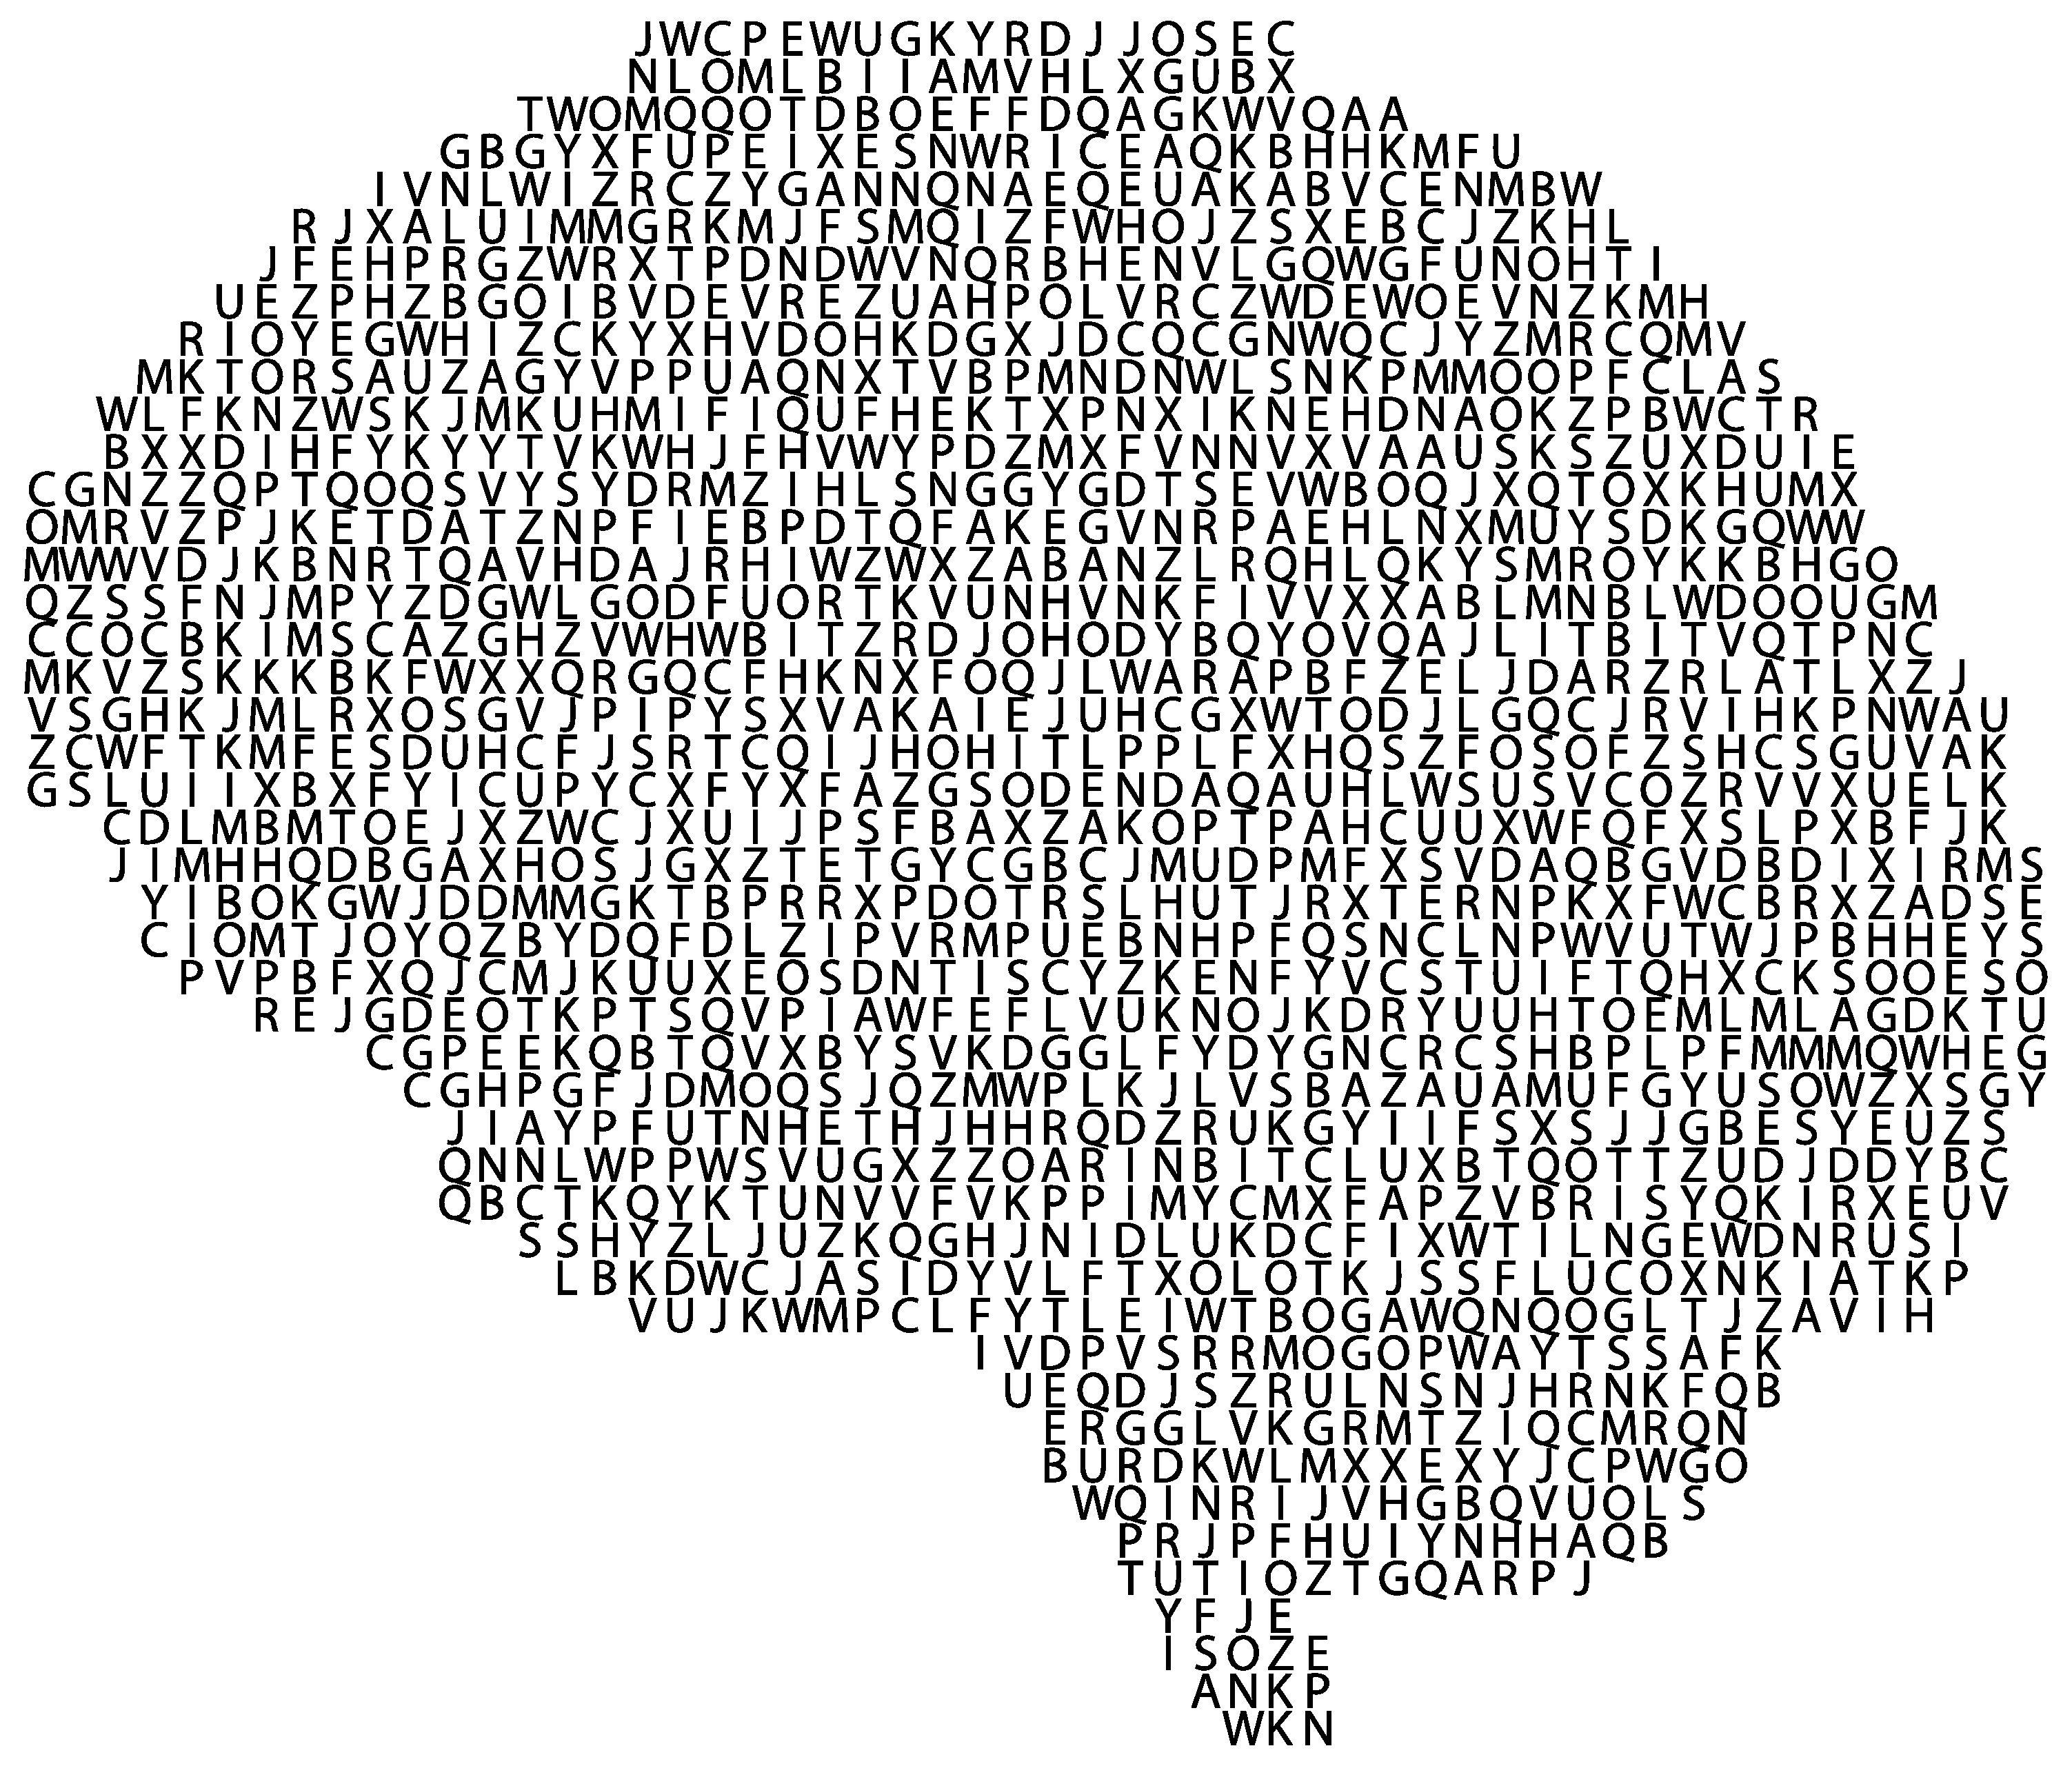
\includegraphics[width=1.6cm]{images/publicdomainvectors_Random-Alphabet-Brain.pdf}
    \end{minipage}
    \hfill
    \begin{minipage}{0.75\textwidth}
      Beim Lernen/Trainieren werden die Parameter einer Funktion
      gesucht. Diese Funktion projeziert die Input-Variablen in $X$
      auf die Ausgabevariable $y$.\\

      $y = f(X)$
    \end{minipage}
    \vspace{0.3cm}
  \end{block}
\end{frame}

\begin{frame}
  \frametitle{Workflow}
  \begin{center}
    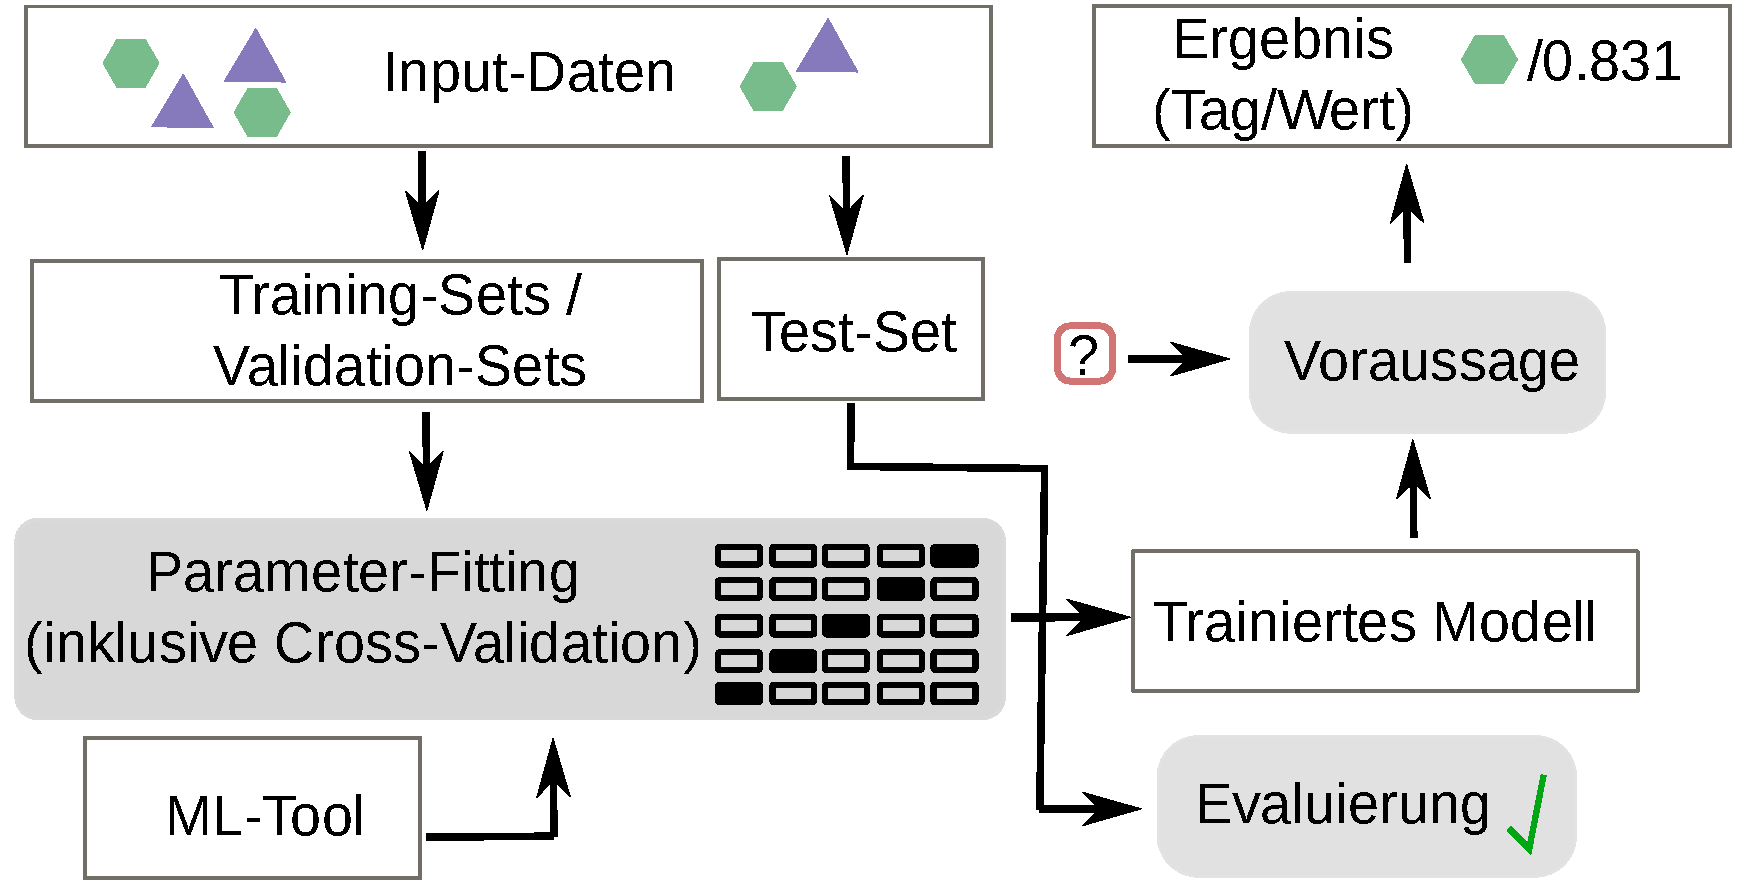
\includegraphics[width=13cm]{images/workflow_training_test_set.pdf}
  \end{center}  
\end{frame}

\begin{frame}
  \frametitle{Wie gut funktioniert eine Methode?}

  \begin{block}{}
    \begin{center}
      \textbf{Überanpassung (Overfitting)}: Modell funktioniert gut
      auf den Trainingsdaten, nicht aber auf anderen Daten.\\
    \end{center}
  \end{block}

  %% \begin{block}{}
  %%   \begin{center}
  %%     \textbf{Regularization}: Verschiedene Methoden dem Overfi\\
  %%   \end{center}
  %% \end{block}
  
  \begin{block}{}
    \begin{center}
      \textbf{Unteranpassung (Underfitting)}: Modell funktioniert
      weder auf den Trainingsdaten noch auf anderen Daten.\\
    \end{center}
  \end{block}
  

  
\end{frame}

%% \begin{frame}
%%   \frametitle{Evaluation of classificaions}

%%   Evaluation of binary classification - Confusion matrix for binary classification
  
%%   \begin{itemize}
%%   \item Positive (P): Observation is positive (for example: is an apple)
%%   \item Negative (N): Observation is not positive (for example: is not an apple).
%%   \item True Positive (TP): Observation is positive, and is predicted to be positive.
%%   \item False Negative (FN): Observation is positive, but is predicted negative.
%%   \item True Negative (TN): Observation is negative, and is predicted to be negative.
%%   \item False Positive (FP): Observation is negative, but is predicted positive.

%%   \item Accuracy
%%     ACC = (TP + TN) / (P + N)

%%   \item Recall sensitivity,  true positive rate
%%     TPR = TP / P

%%   \item Precision /  positive predictive value
%%     PPV = TP / (TP + FP)

%%   \item F1 (aka F-measure, F-score) - harmonic mean of precision and recall

%%     F1 = 2 * (1 / (1/recall) + (1/recall))
%%   \end{itemize}
  
%% \end{frame}


\begin{frame}
  \frametitle{Ausgewählte überwachte Lernmethoden}
  \begin{block}{}
    \begin{center}
      \begin{itemize}
      \item Nächste-Nachbarn-Methoden (k-Nearest Neighbors)
      \item Naïve Bayes-Klassifikator
      \item Lineare Regression
      \item Logistische Regression
      \item Entscheidungsbäume (Decision Trees)
      \item Künstliche Neuronale Netze (Artificial neural network,
        Multilayer Perceptron)
      \end{itemize}
    \end{center}    
  \end{block}
\end{frame}

%%%%%%%%%%%%%%%%%%%%%%%%%%%%%%%%%%%%%%%%%%%%%%
%\subsection{Ausgewählte überwachte Lernverfahren}
%%%%%%%%%%%%%%%%%%%%%%%%%%%%%%%%%%%%%%%%%%%%%%

%-------------------------------
\subsection{Nächste-Nachbarn-Methoden (k-Nearest Neighbors)}
%-------------------------------

\setcounter{tocdepth}{2}
\begin{frame}{}
   \tableofcontents[currentsubsection,hideothersubsections,
     subsectionstyle=show/shaded]
\end{frame}

\begin{frame}
  \frametitle{Nächste-Nachbarn-Methoden (k-Nearest Neighbors)}
  \begin{block}{}
    \begin{center}
      \begin{itemize}
      \item Für Klassifikation und Regression
      \item Das einfachste maschinelle Lernverfahren
      \item Kann auch für multiple Klassifikation genutzt werden
      \item Zu setzender Parameter: Anzahl der zu beachtenden Nachbarn
      \end{itemize}
    \end{center}
  \end{block}    
\end{frame}

\begin{frame}
  \frametitle{Nächste-Nachbarn-Klassifikation}
  \begin{center}
    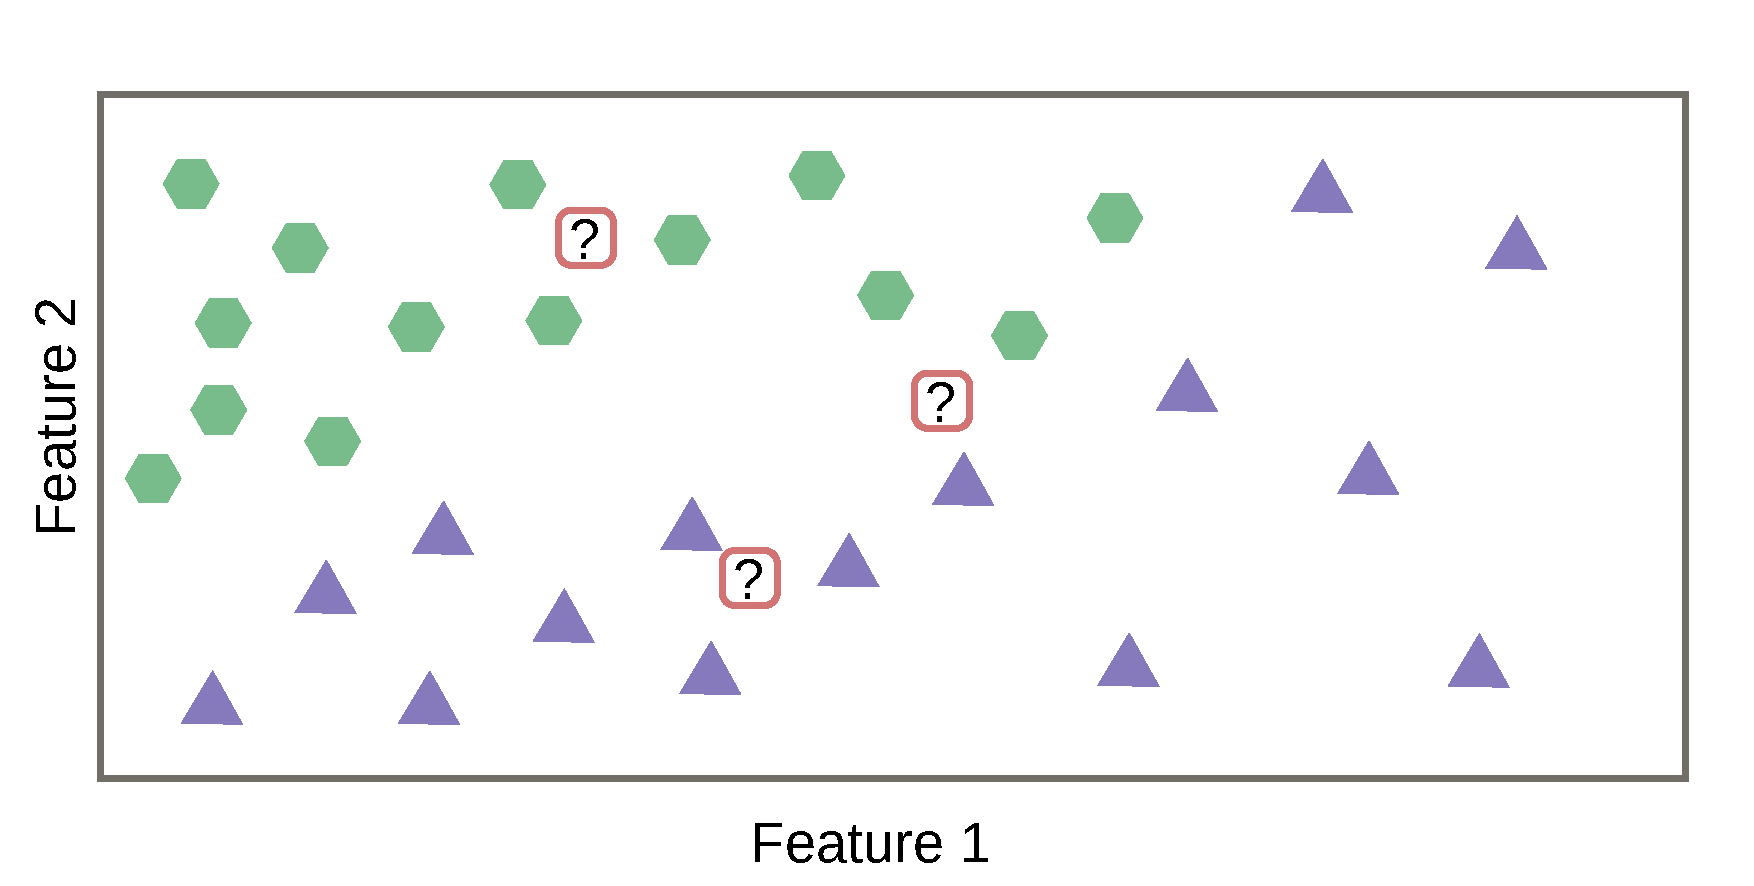
\includegraphics[width=13.0cm]{images/k_nearest_neighbour_classification_only_training_data.pdf}
  \end{center}
\end{frame}

\begin{frame}
  \frametitle{Nächste-Nachbarn-Klassifikation}
  \begin{center}
    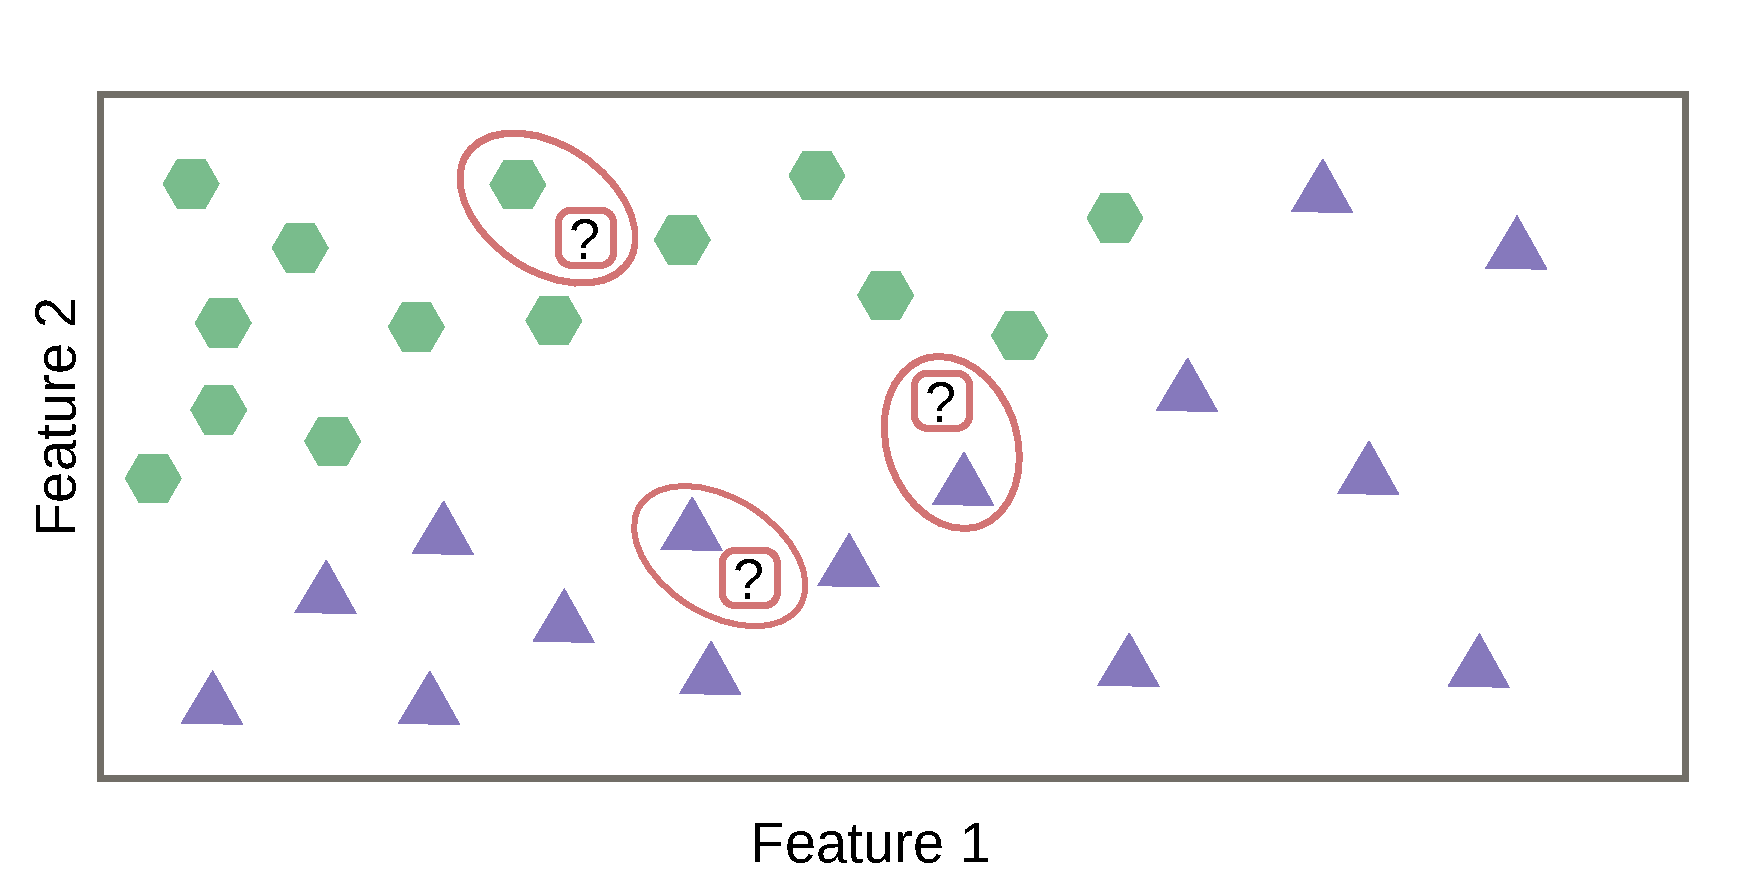
\includegraphics[width=13.0cm]{images/k_nearest_neighbour_classification_k_1.pdf}
  \end{center}
\end{frame}

\begin{frame}
  \frametitle{Nächste-Nachbarn-Klassifikation}
  \begin{center}
    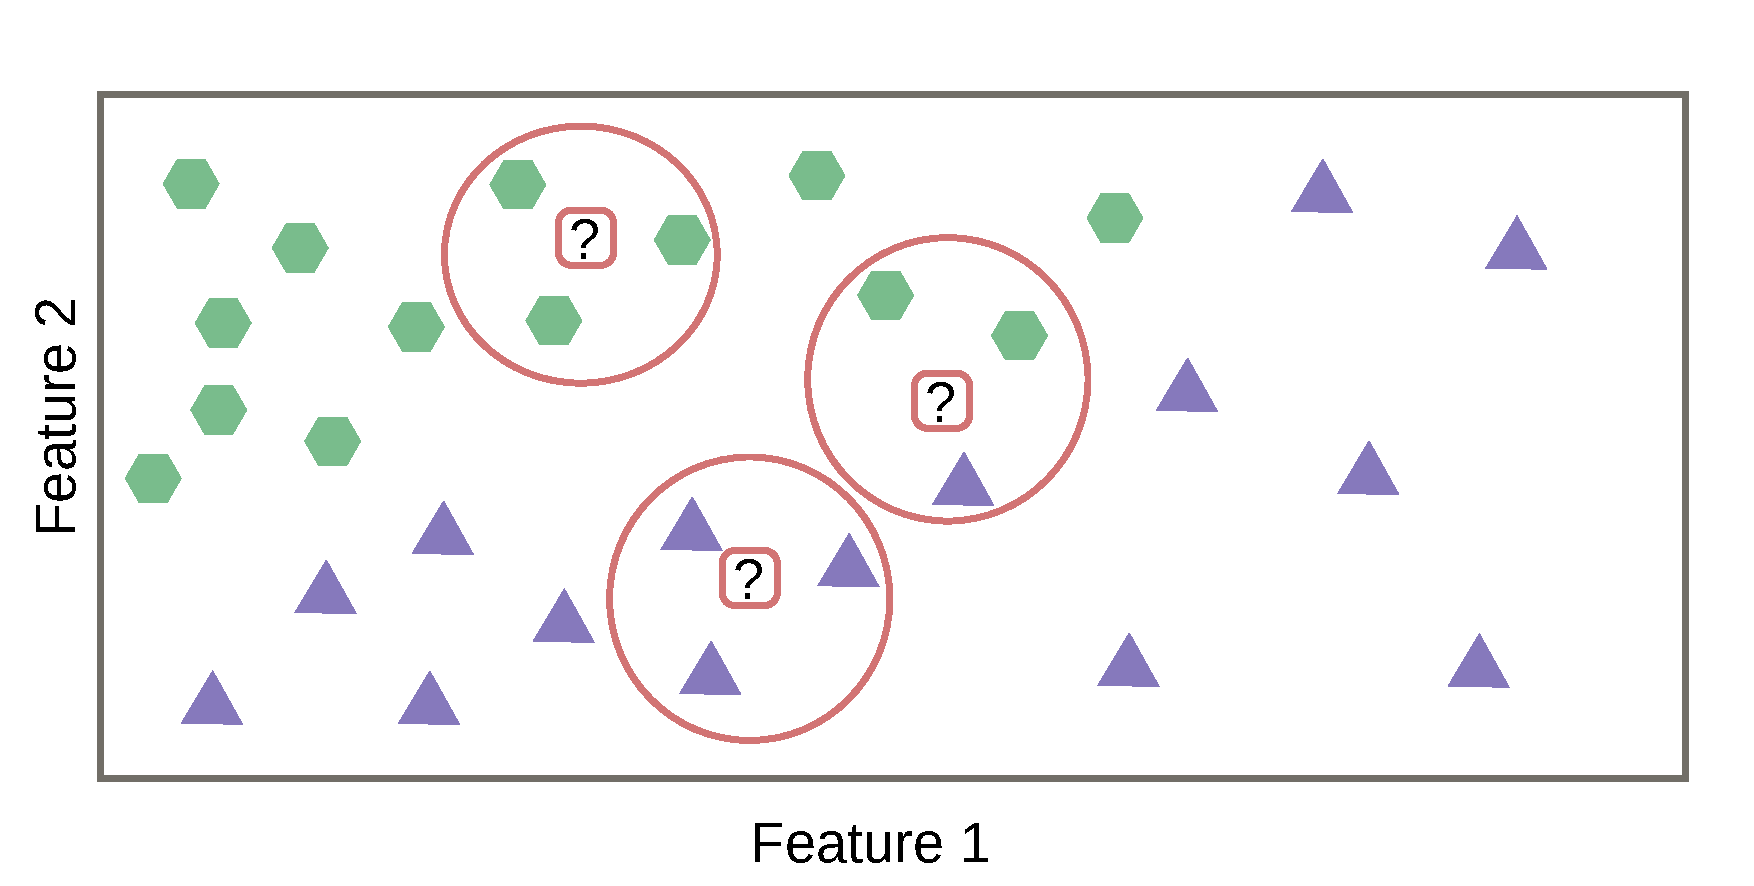
\includegraphics[width=13.0cm]{images/k_nearest_neighbour_classification_k_3.pdf}
  \end{center}
\end{frame}

\begin{frame}
  \frametitle{Nächste-Nachbarn-Regression}
  \begin{center}
    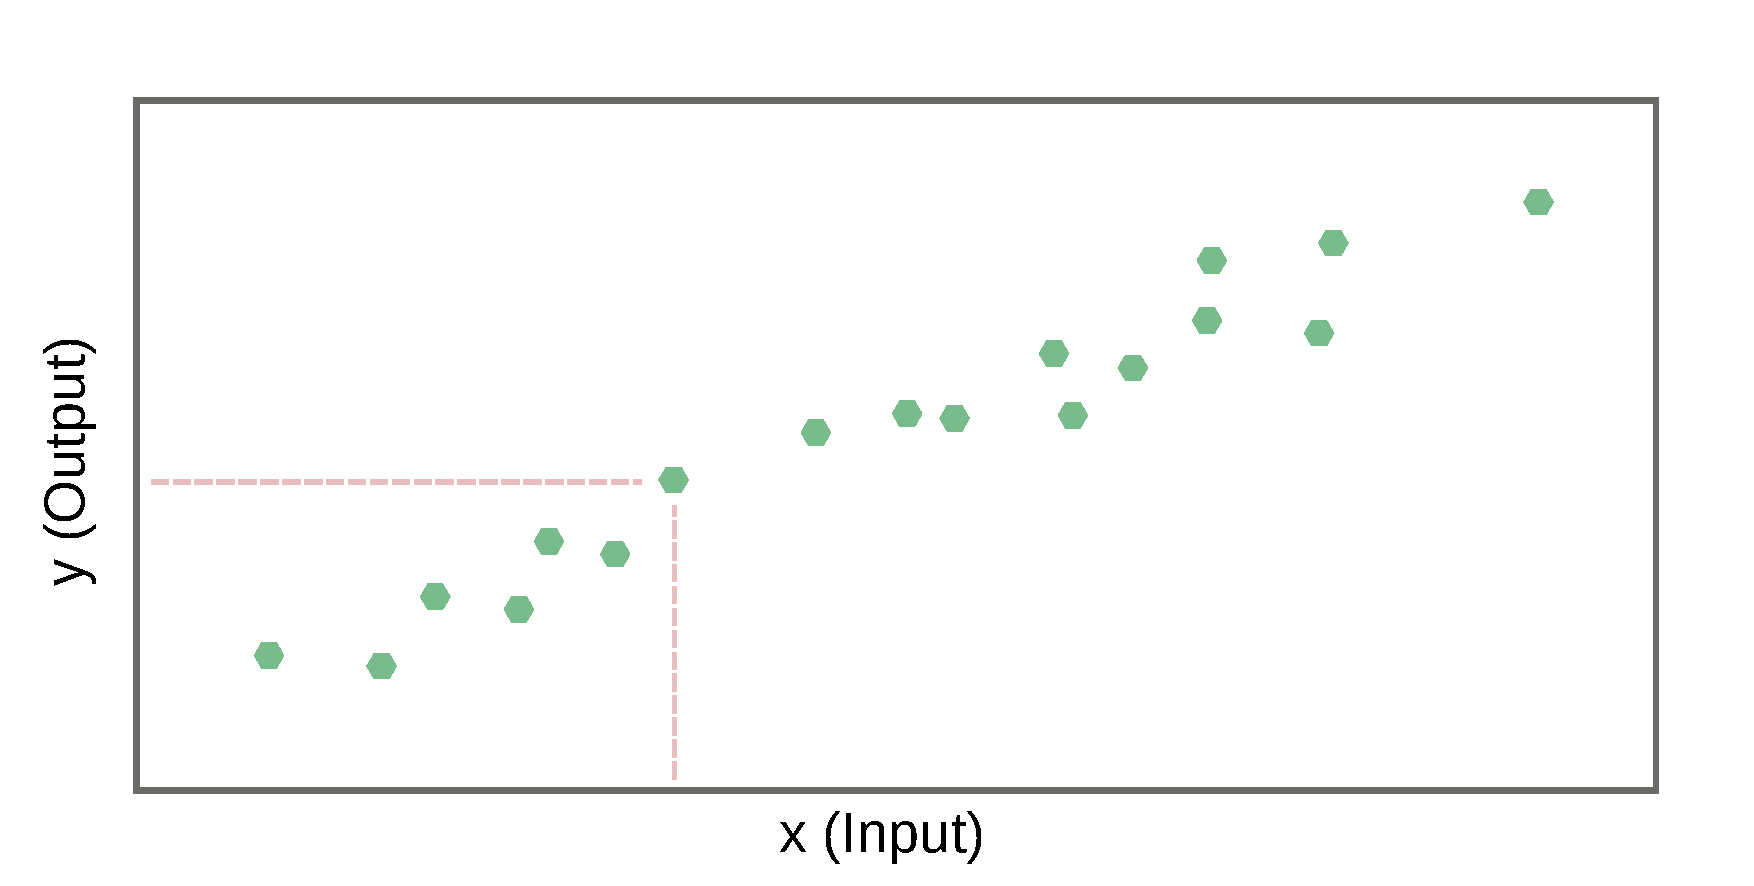
\includegraphics[width=13.0cm]{images/k_nearest_neighbour_regression_only_training_data.pdf}
  \end{center}
\end{frame}

\begin{frame}
  \frametitle{Nächste-Nachbarn-Regression}
  \begin{center}
    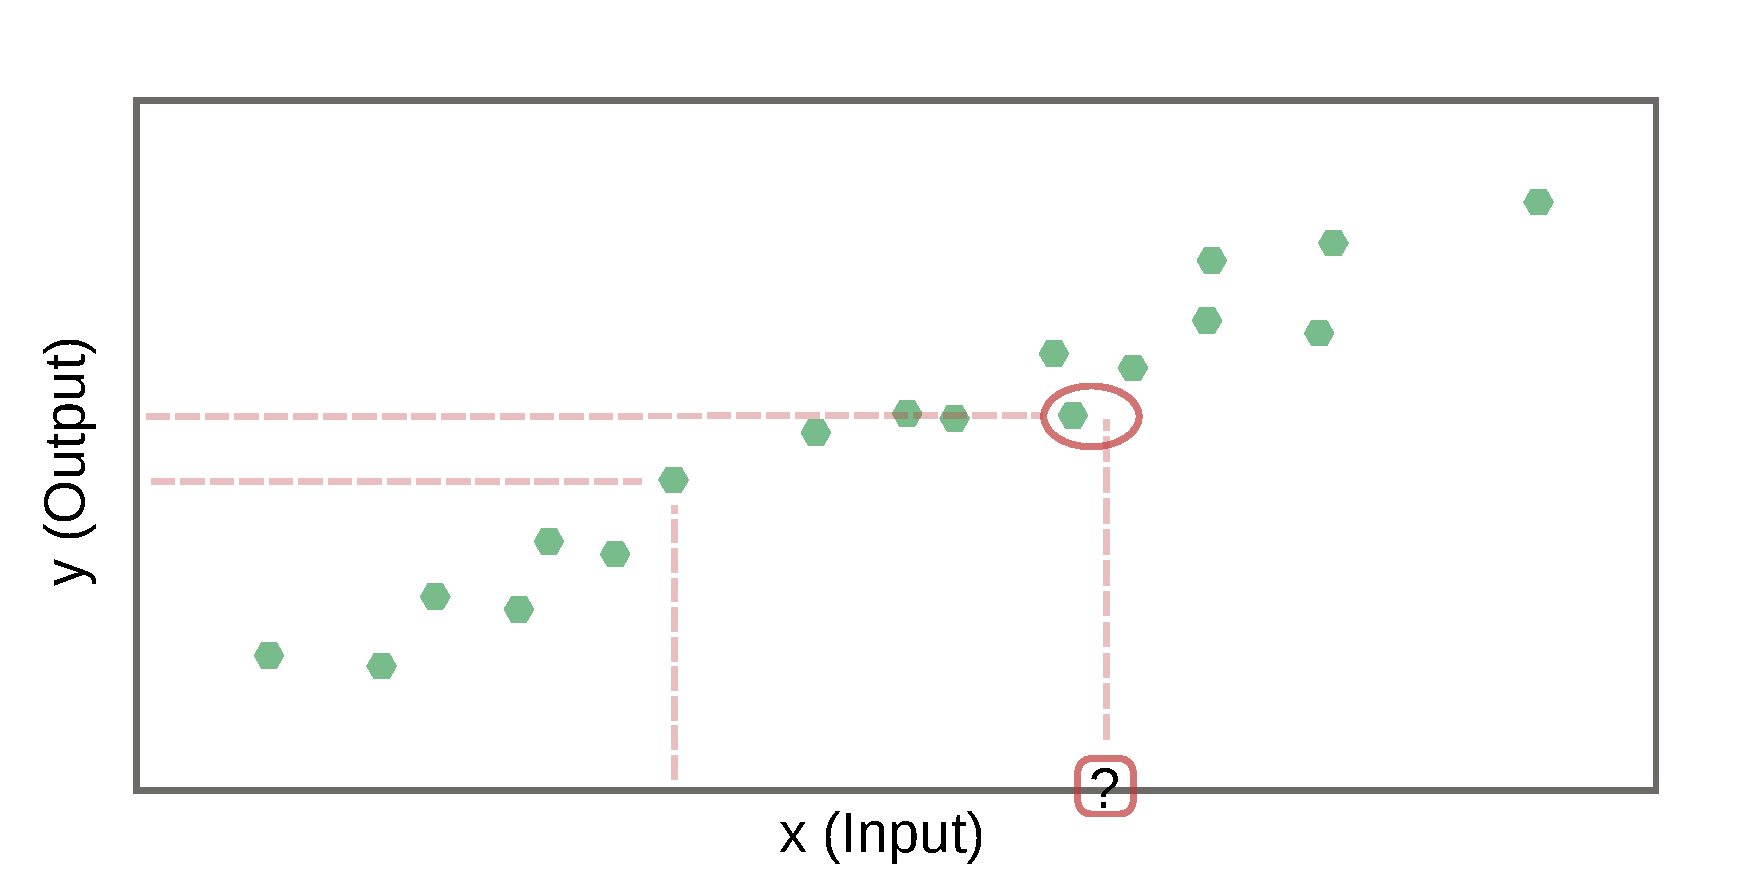
\includegraphics[width=13.0cm]{images/k_nearest_neighbour_regression_k_1.pdf}    
  \end{center}
\end{frame}

\begin{frame}
  \frametitle{Nächste-Nachbarn-Klassifikation}
  \begin{center}
    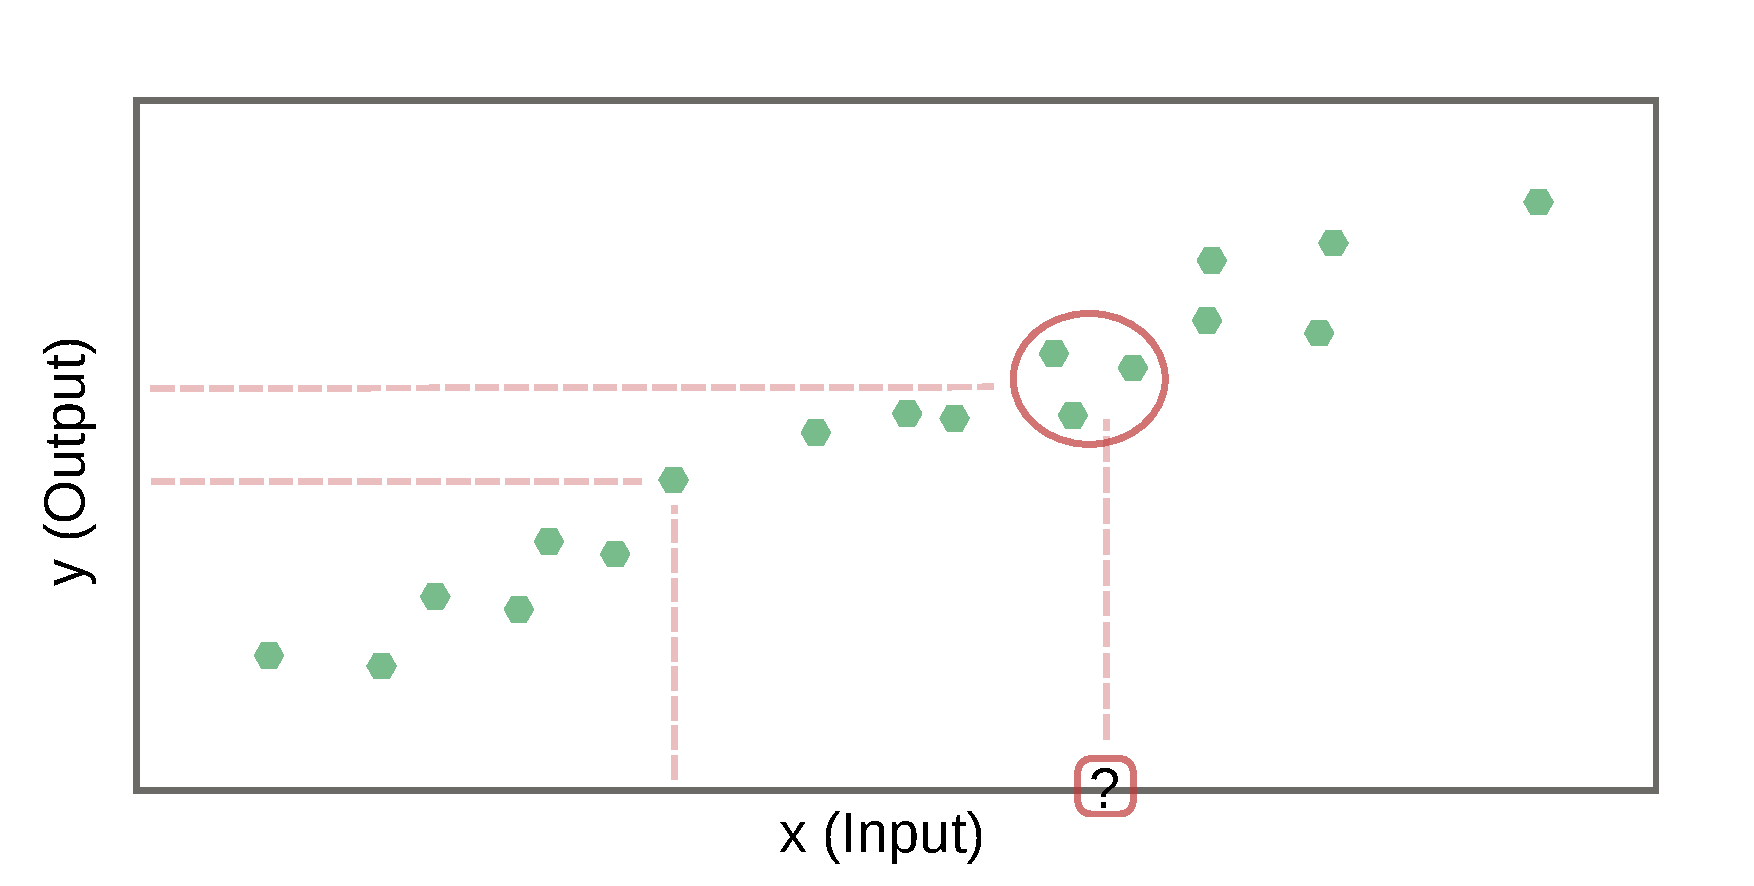
\includegraphics[width=13.0cm]{images/k_nearest_neighbour_regression_k_3.pdf}
  \end{center}
\end{frame}


%-------------------------
\subsection{Lineare Modelle}
%-------------------------

\setcounter{tocdepth}{2}
\begin{frame}{}
   \tableofcontents[currentsubsection,hideothersubsections,
     subsectionstyle=show/shaded]
\end{frame}

\begin{frame}
  \frametitle{Lineare Modelle}  
  \begin{block}{}
    \begin{itemize}
    \item Für Klassifikation und Regression
    \item Nur für lineare Probleme
    \item I.a. einfach und schnell
    \end{itemize}
  \end{block}
\end{frame}

\begin{frame}
  \frametitle{Lineare Modelle}
  \begin{center}
    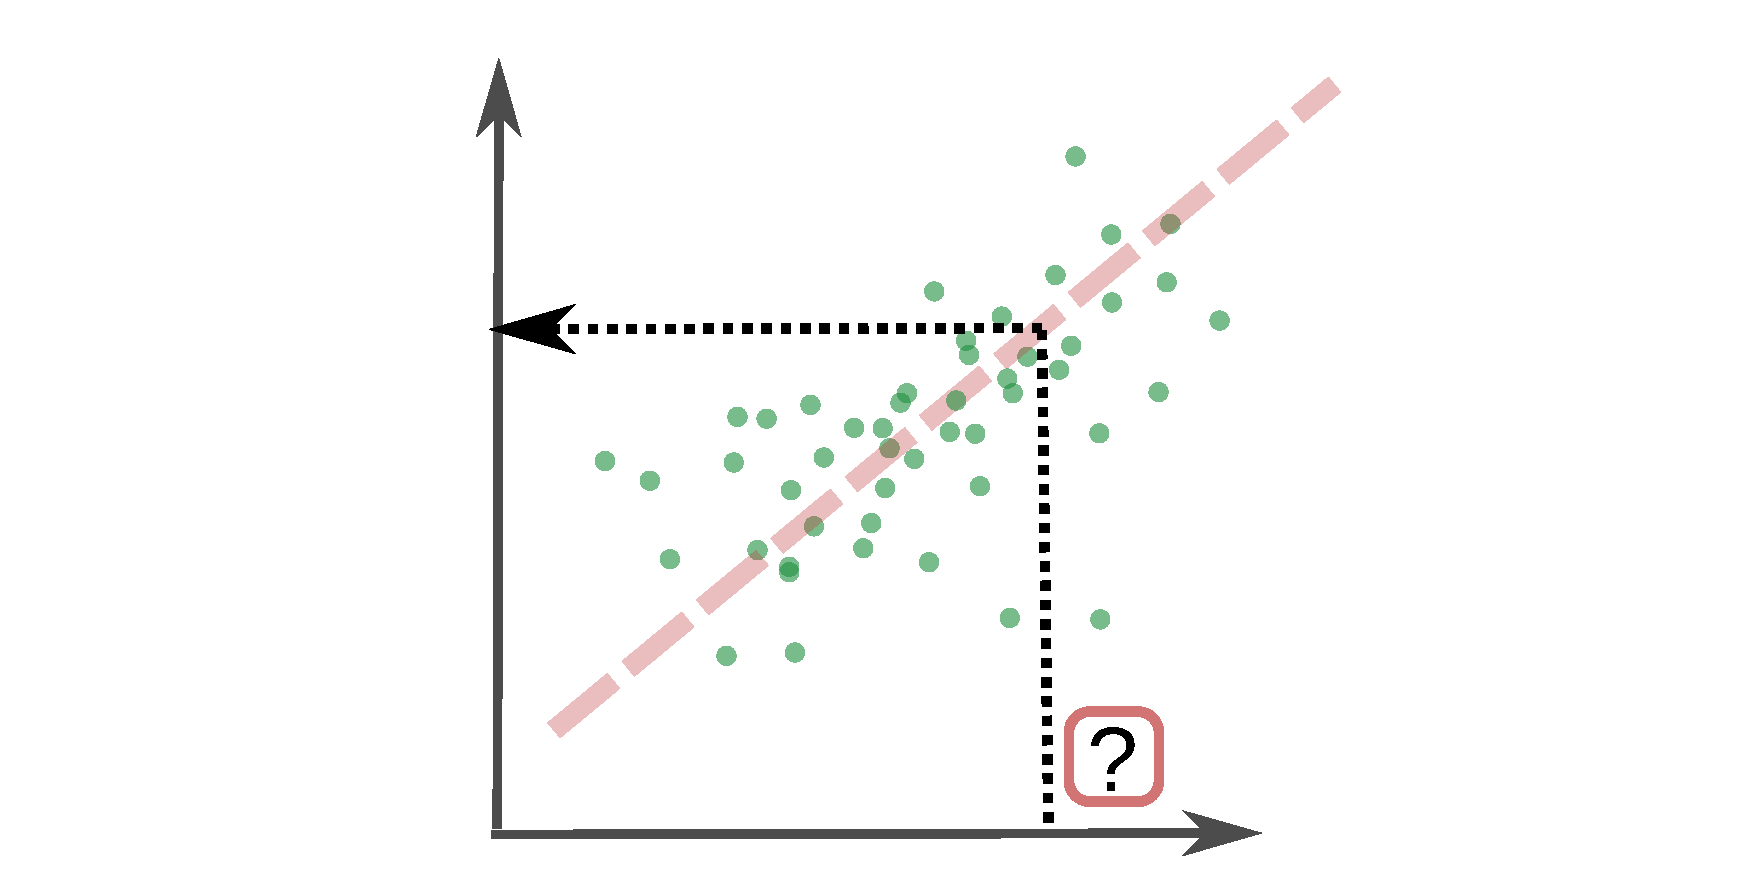
\includegraphics[width=13.0cm]{images/Linear_Regression.pdf}
  \end{center}
\end{frame}

\begin{frame}
  \frametitle{Lineare Modelle}
  \begin{block}{}
    \begin{center}
      $\hat{y} = w_{1}x_{1} + w_{2}x_{2} + w_{3}x_{3} + ... + w_{n}x_{n} + b$\\
      \ \\
      mit $n$ als Zahl der Eigenschaften,\\
      $w$'s als Parameter/Wichtungen/Koeffizienten\\ und
      $b$ als Y-Achsenabschnitt (Intercept)\\
      ($\hat{y}$ - "y Dach" / englisch "y hat")
    \end{center}
  \end{block}  
\end{frame}

\begin{frame}
  \frametitle{Verschiedene Wege die Koeffizienten zu berechnen}
  \begin{block}{}
    \begin{center}
      \begin{itemize}
      \item Methode der kleinsten Quadrate (Ordinary Least Squares, OLS)
        \begin{itemize}
        \item Keine Parameter aber einfach anzupassen
        \end{itemize}
      \item Ridge
        \begin{itemize}
        \item Stabiler gegen Overfitting
        \end{itemize}    
      \item Least Absolute Shrinkage and Selection Operator (LASSO)
      \end{itemize}
    \end{center}
  \end{block}
\end{frame}

\begin{frame}
  \frametitle{Methode der kleinsten Quadrate}
  \begin{center}
    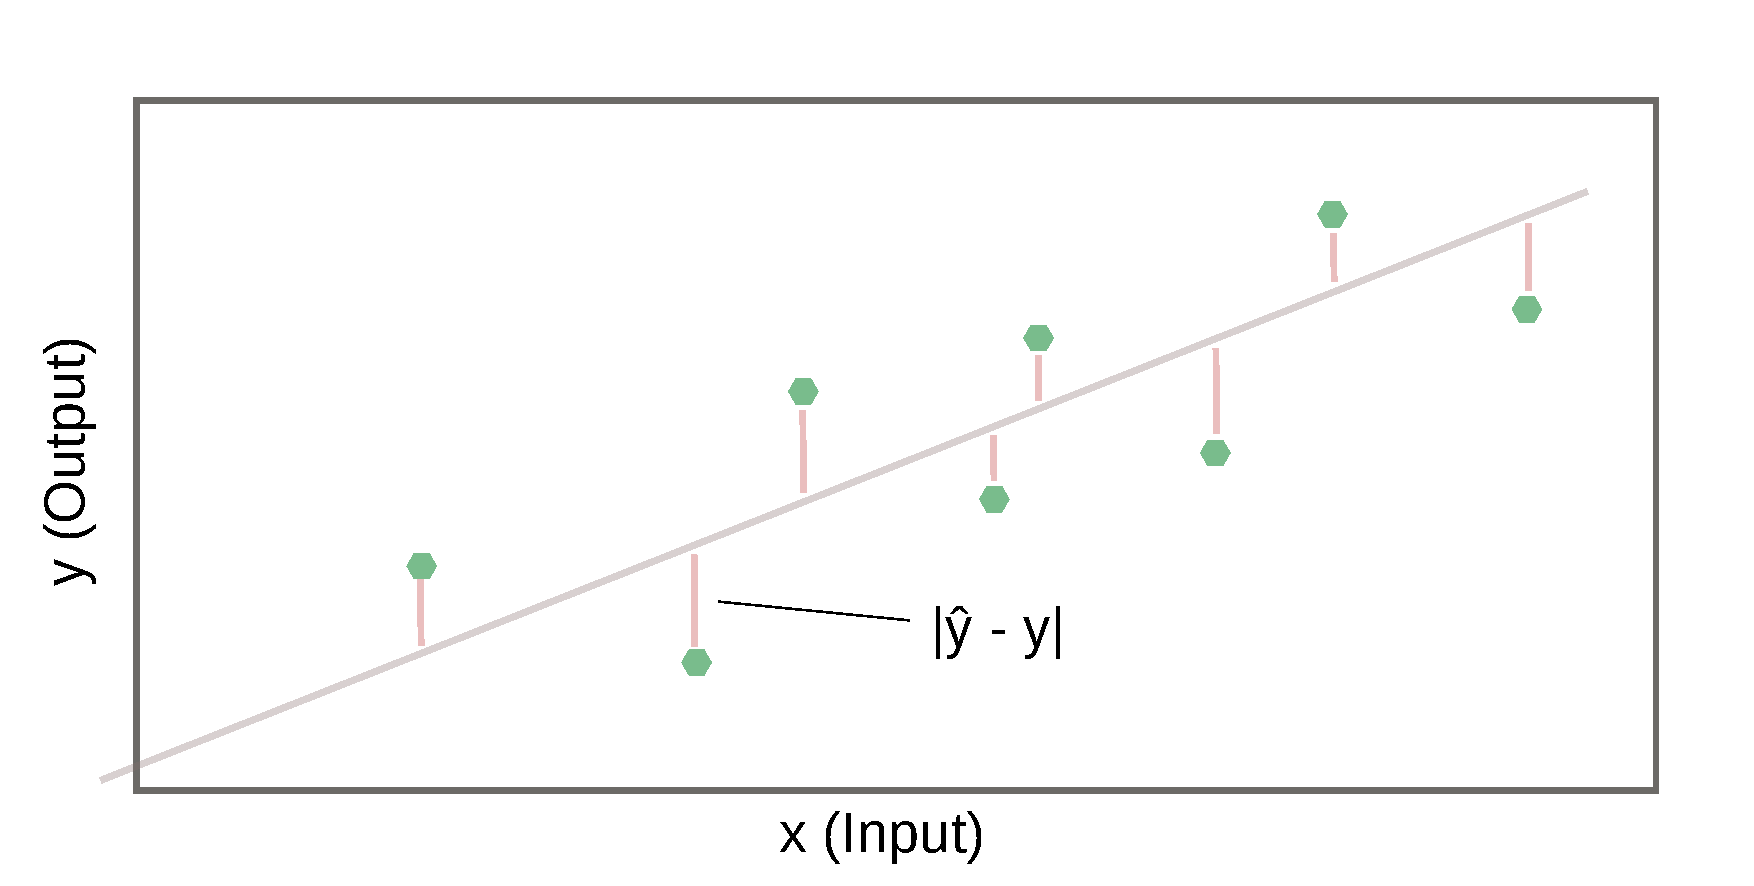
\includegraphics[width=13.0cm]{images/linear_model_ordinary_least_squares.pdf}
    Minimierung der Differenz von $\hat{y}$ and $y$.
  \end{center}
\end{frame}

\begin{frame}
  \frametitle{}
  \begin{block}{}
    \begin{center}
      Wenn die Parameter ($b$ and die $w$-Werte) \\
      geschätzt wurden, kann man Voraussagen durchführen indem\\ man
      die Attribute-Werte entsprechend einsetzt und somit $\hat{y}$
      berechnet. \\ \ \\
      $\hat{y} = w_{1}x_{1} + w_{2}x_{2} + w_{3}x_{3} + ... + w_{n}x_{n} + b$\\
    \end{center}
  \end{block}
\end{frame}

%-----------------------------------------
\subsection{Support Vector Machines (SVMs)}
%-----------------------------------------

\setcounter{tocdepth}{2}
\begin{frame}{}
   \tableofcontents[currentsubsection,hideothersubsections,
     subsectionstyle=show/shaded]
\end{frame}

\begin{frame}
  \frametitle{Support Vector Machines (SVMs)}  
  \begin{block}{}
    \begin{itemize}
    \item Für Klassifikation und Regression
    \item Auch für nicht-lineare Probleme
    \end{itemize}
  \end{block}
\end{frame}

\begin{frame}
  \frametitle{Support Vector Machines (SVMs) -- Teilende Hyperebene}
  \begin{center}
    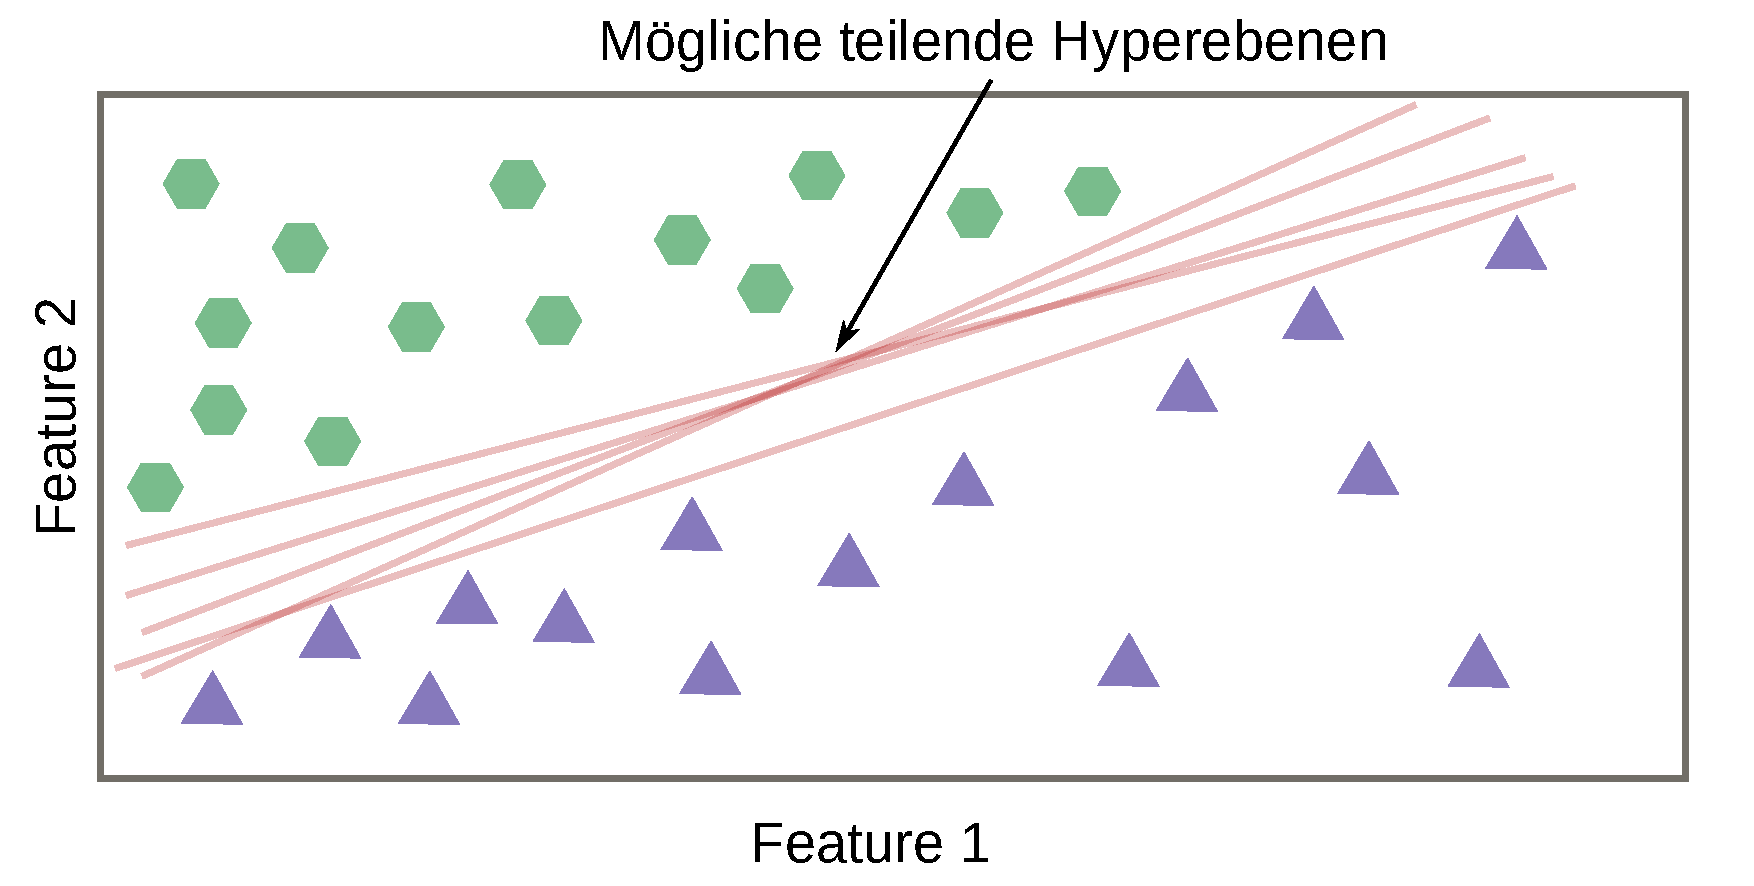
\includegraphics[width=13.0cm]{images/svm_potential_separating_hyperplanes.pdf}
  \end{center}
\end{frame}

\begin{frame}
  \frametitle{Support Vector Machines (SVMs) -- Margin/Support-Vektoren}
  \begin{center}
    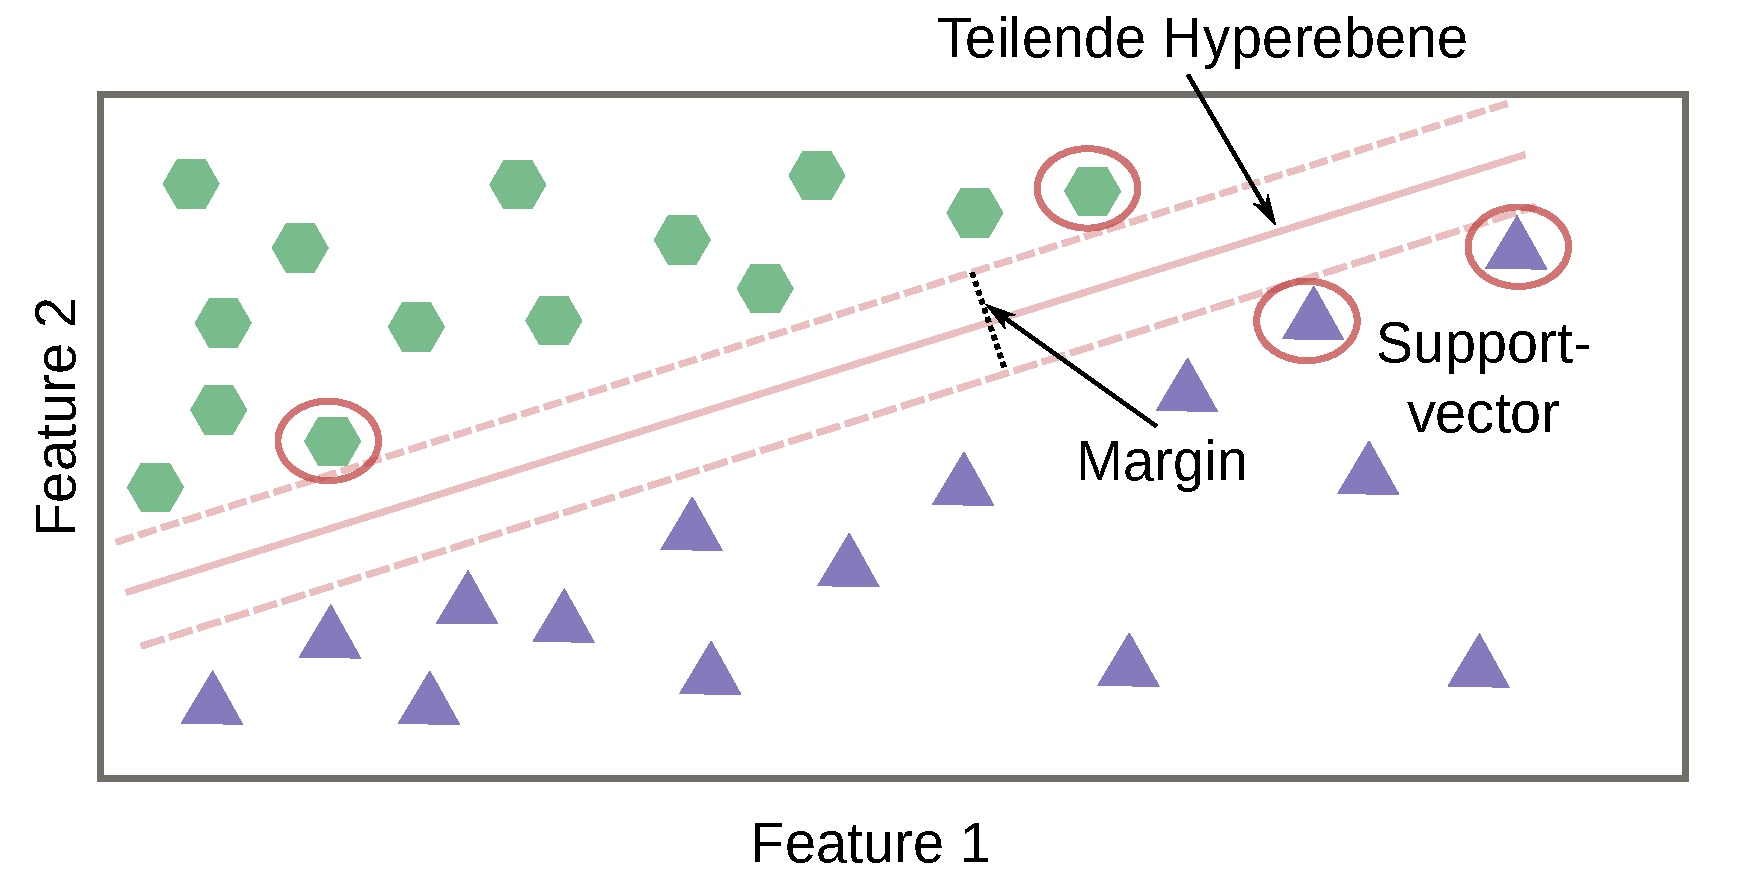
\includegraphics[width=13.0cm]{images/svm_with_margin.pdf}
  \end{center}
\end{frame}

\begin{frame}
  \frametitle{Support Vector Machines (SVMs) -- Soft Margin}
  \begin{center}
    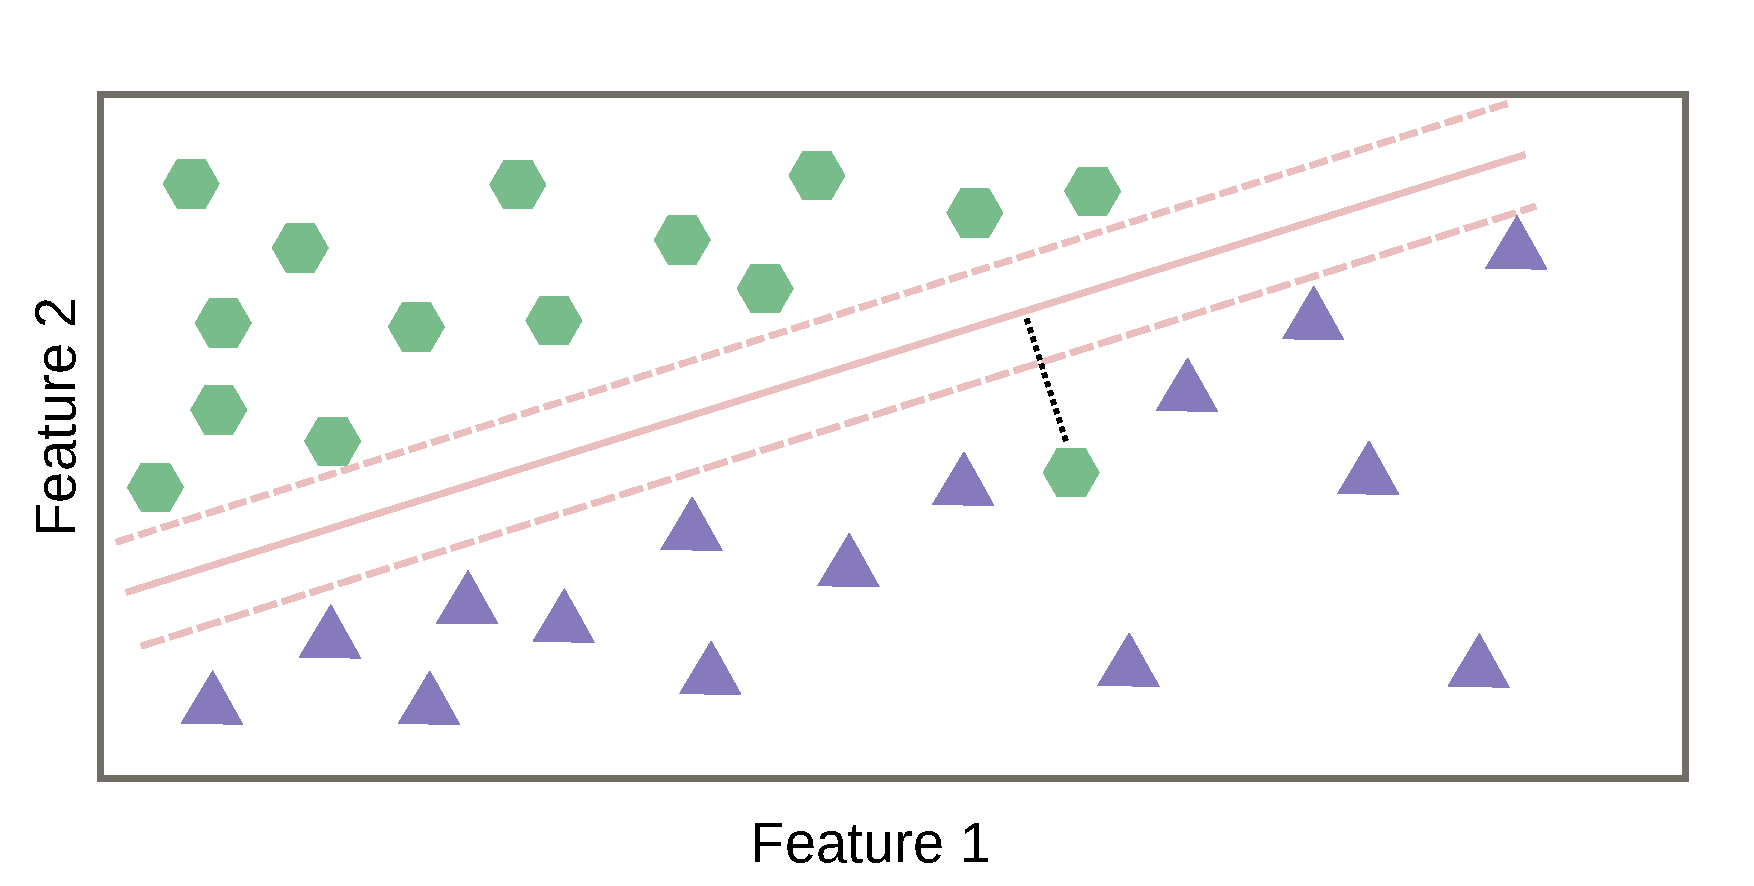
\includegraphics[width=13.0cm]{images/svm_with_soft_margin.pdf}
  \end{center}
\end{frame}

\begin{frame}
  \frametitle{Support Vector Machines (SVMs) -- Kernel-Trick}
  \begin{center}
    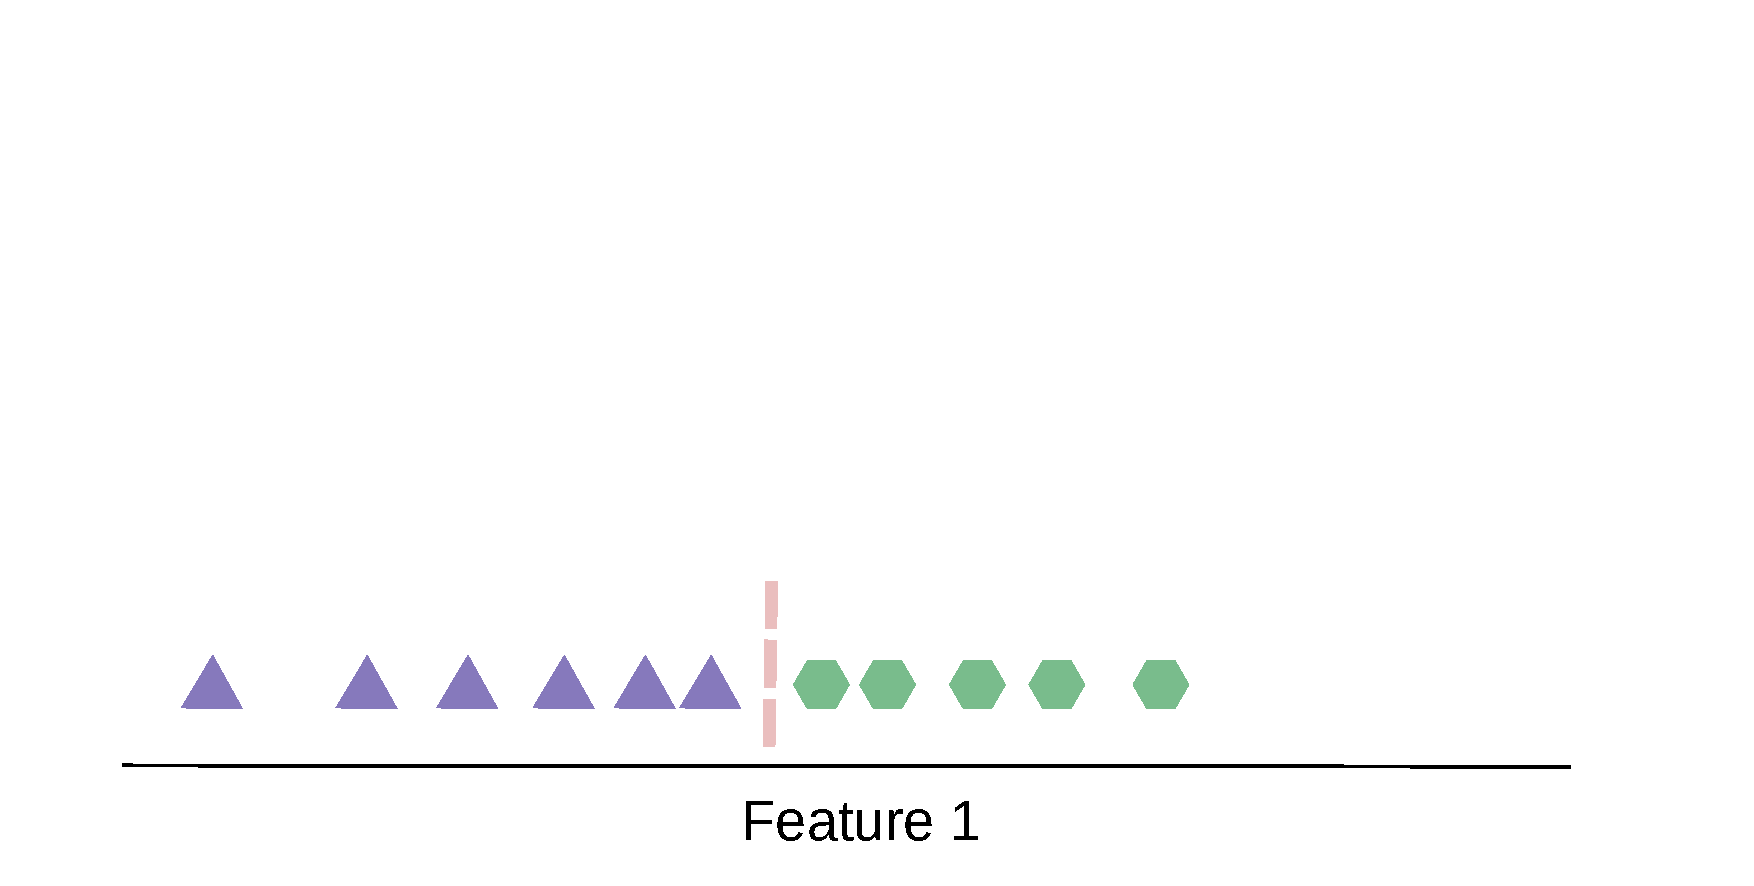
\includegraphics[width=13.0cm]{images/svm_kernel_trick_1.pdf}
  \end{center}
\end{frame}

\begin{frame}
  \frametitle{Support Vector Machines (SVMs) -- Kernel trick}
  \begin{center}
    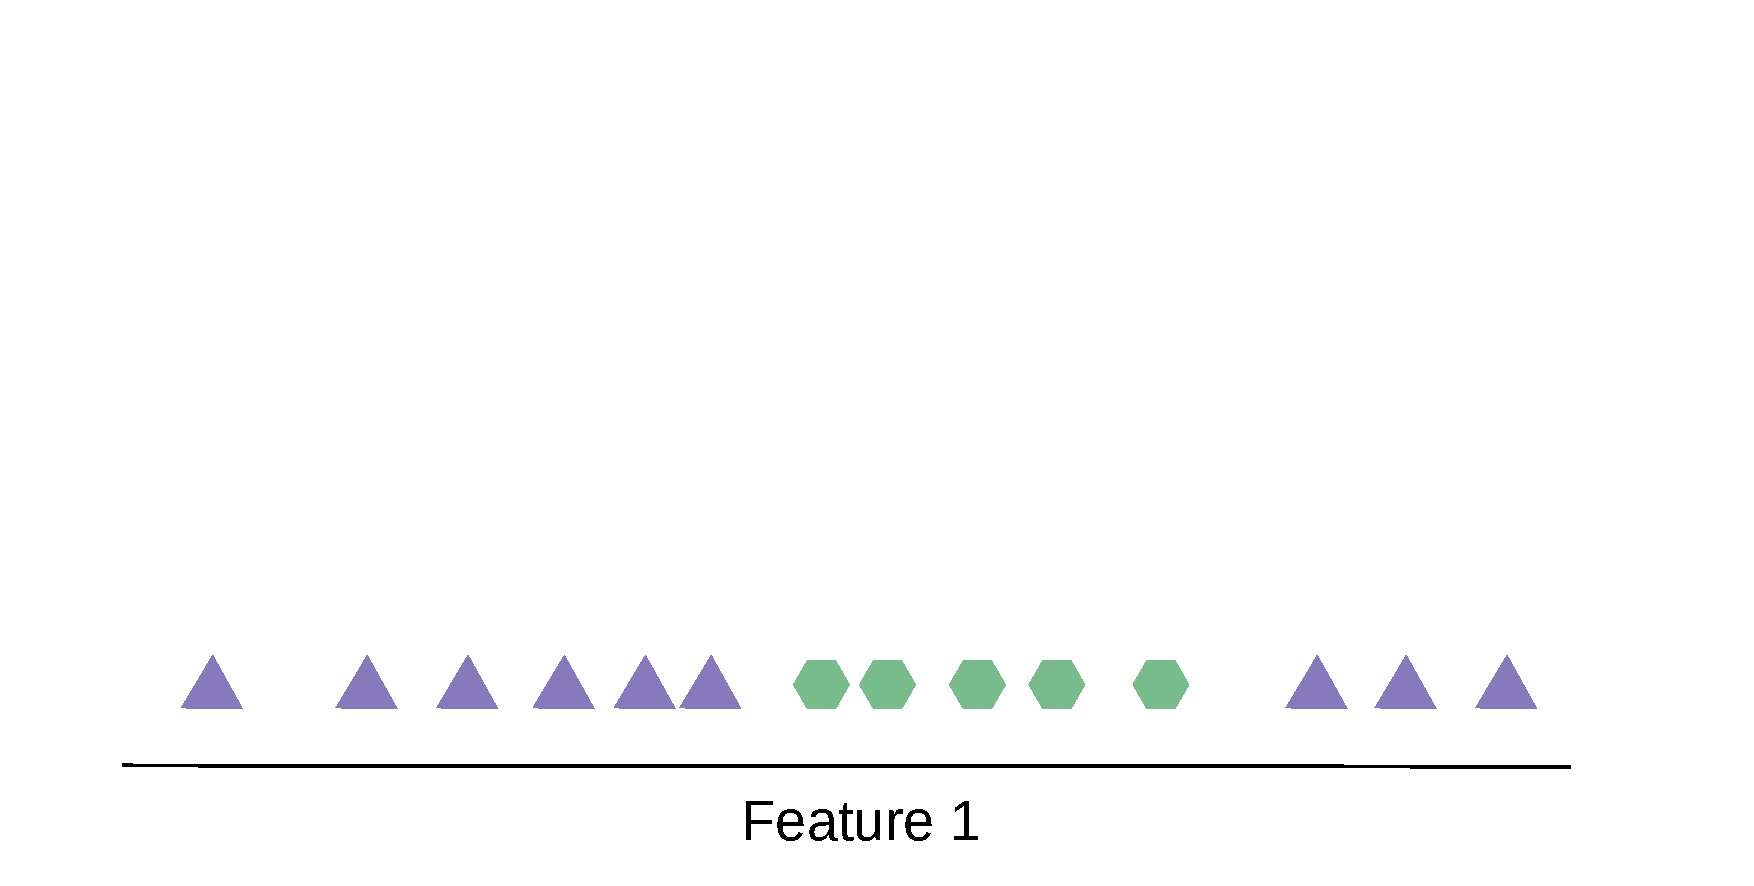
\includegraphics[width=13.0cm]{images/svm_kernel_trick_2.pdf}
  \end{center}
\end{frame}

\begin{frame}
  \frametitle{Support Vector Machines (SVMs) -- Kernel trick}
  \begin{center}
    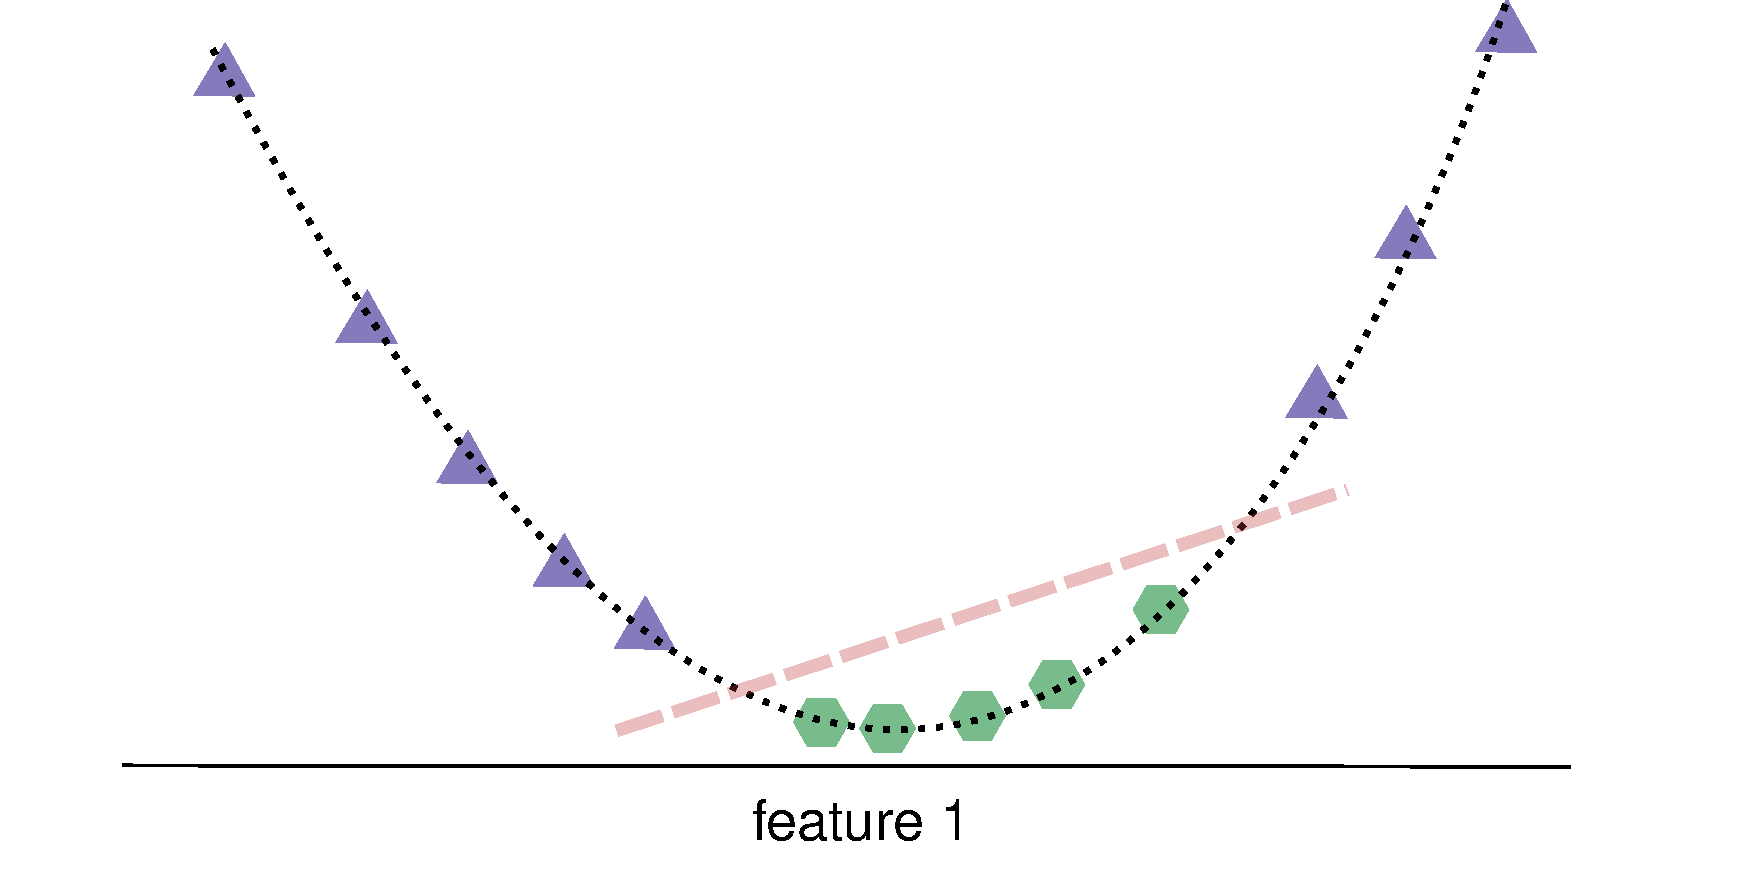
\includegraphics[width=13.0cm]{images/svm_kernel_trick_3.pdf}
  \end{center}
\end{frame}

%-------------------------
\subsection{Entscheidungsbäume (Decision trees) und Random forest}
%-------------------------

\setcounter{tocdepth}{2}
\begin{frame}{}
  \tableofcontents[currentsubsection,hideothersubsections,
    subsectionstyle=show/shaded]
\end{frame}

\begin{frame}
  \frametitle{Entscheidungsbäume (Decision Trees)}
  \begin{block}{}
    \vspace{0.5cm}
    \begin{minipage}{0.2\textwidth}
      \ \ \ \ \ \ \
      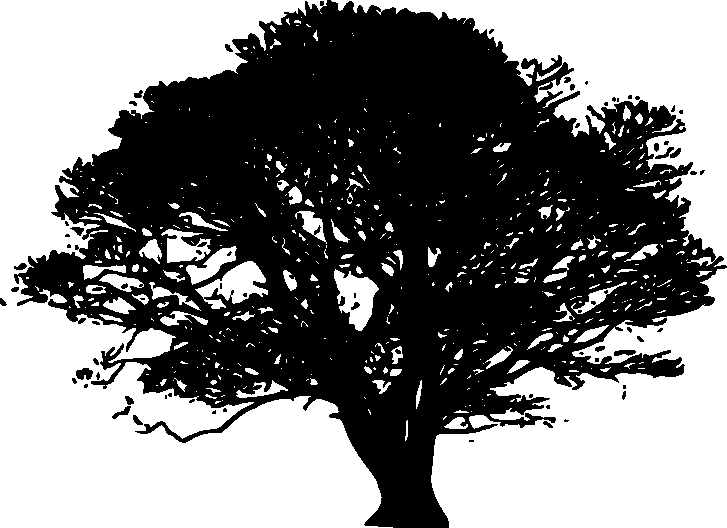
\includegraphics[width=1.6cm]{images/publicdomainvectors_Chrisdesign_Tree_silhouettes_5.pdf}
    \end{minipage}
    \hfill
    \begin{minipage}{0.7\textwidth}
      \begin{itemize}
      \item Für Klassifikation und Regression
      \item Auch für nicht-lineare Probleme
      \item Parameter gut nachvollziehbar
      \end{itemize}
    \end{minipage}
    \vspace{0.5cm}
  \end{block}
\end{frame}

\begin{frame}
  \frametitle{Entscheidungsbäume (Decision Trees)}
  \begin{center}
    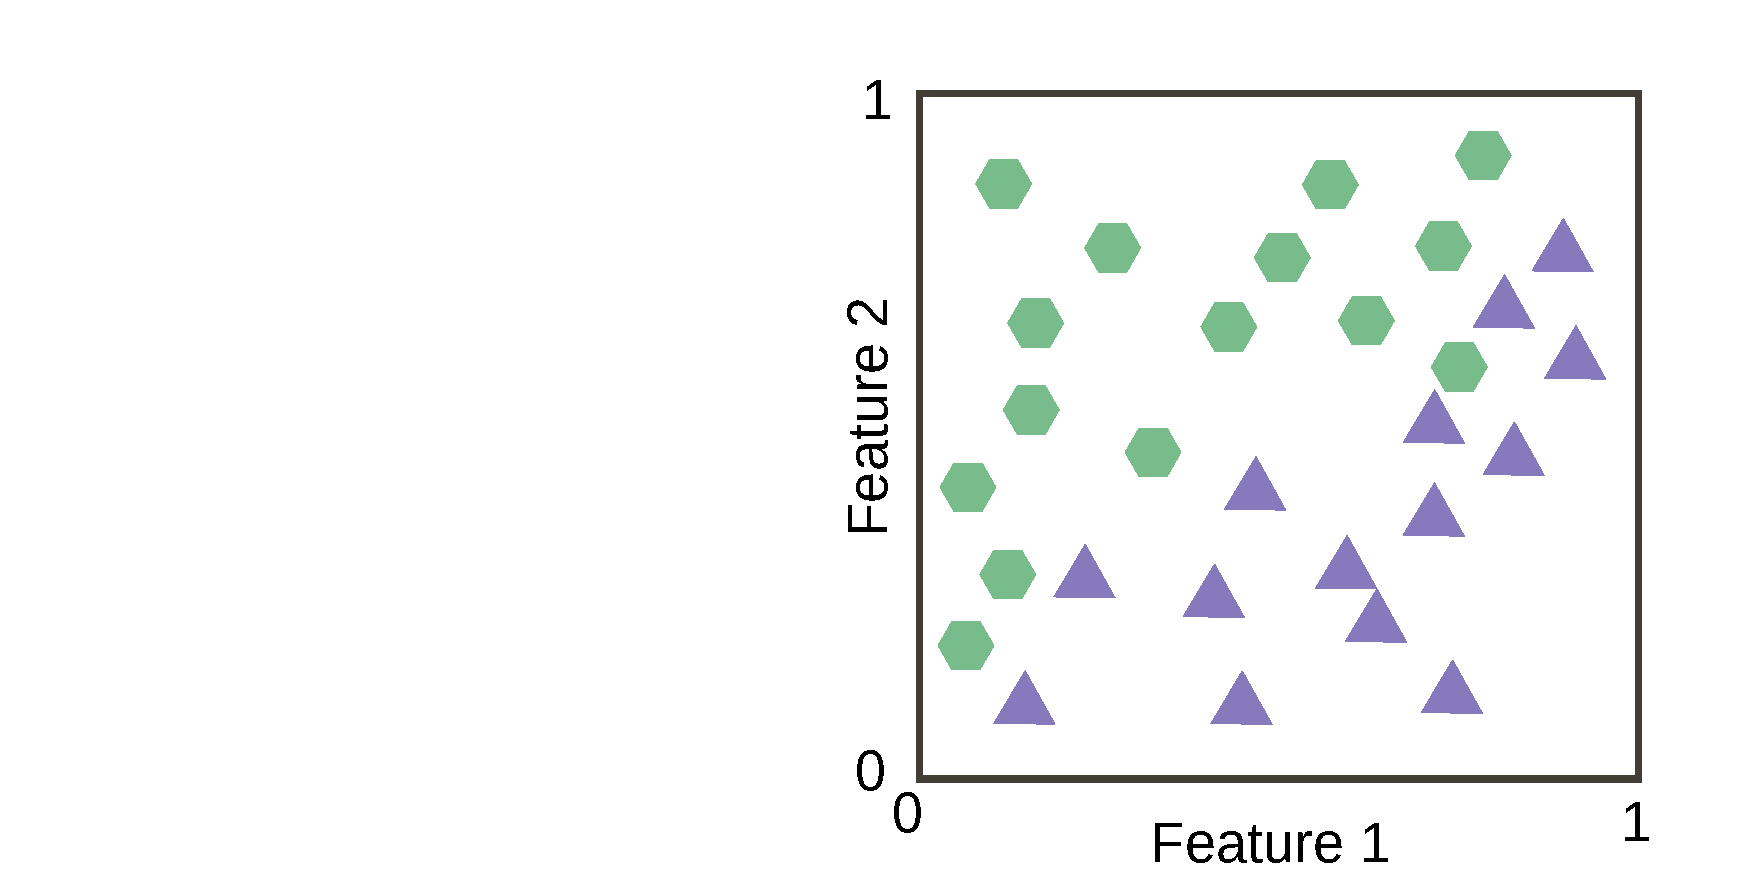
\includegraphics[width=13.0cm]{images/decision_tree_0.pdf}
  \end{center}  
\end{frame}

\begin{frame}
  \frametitle{Entscheidungsbäume (Decision Trees)}
  \begin{center}
    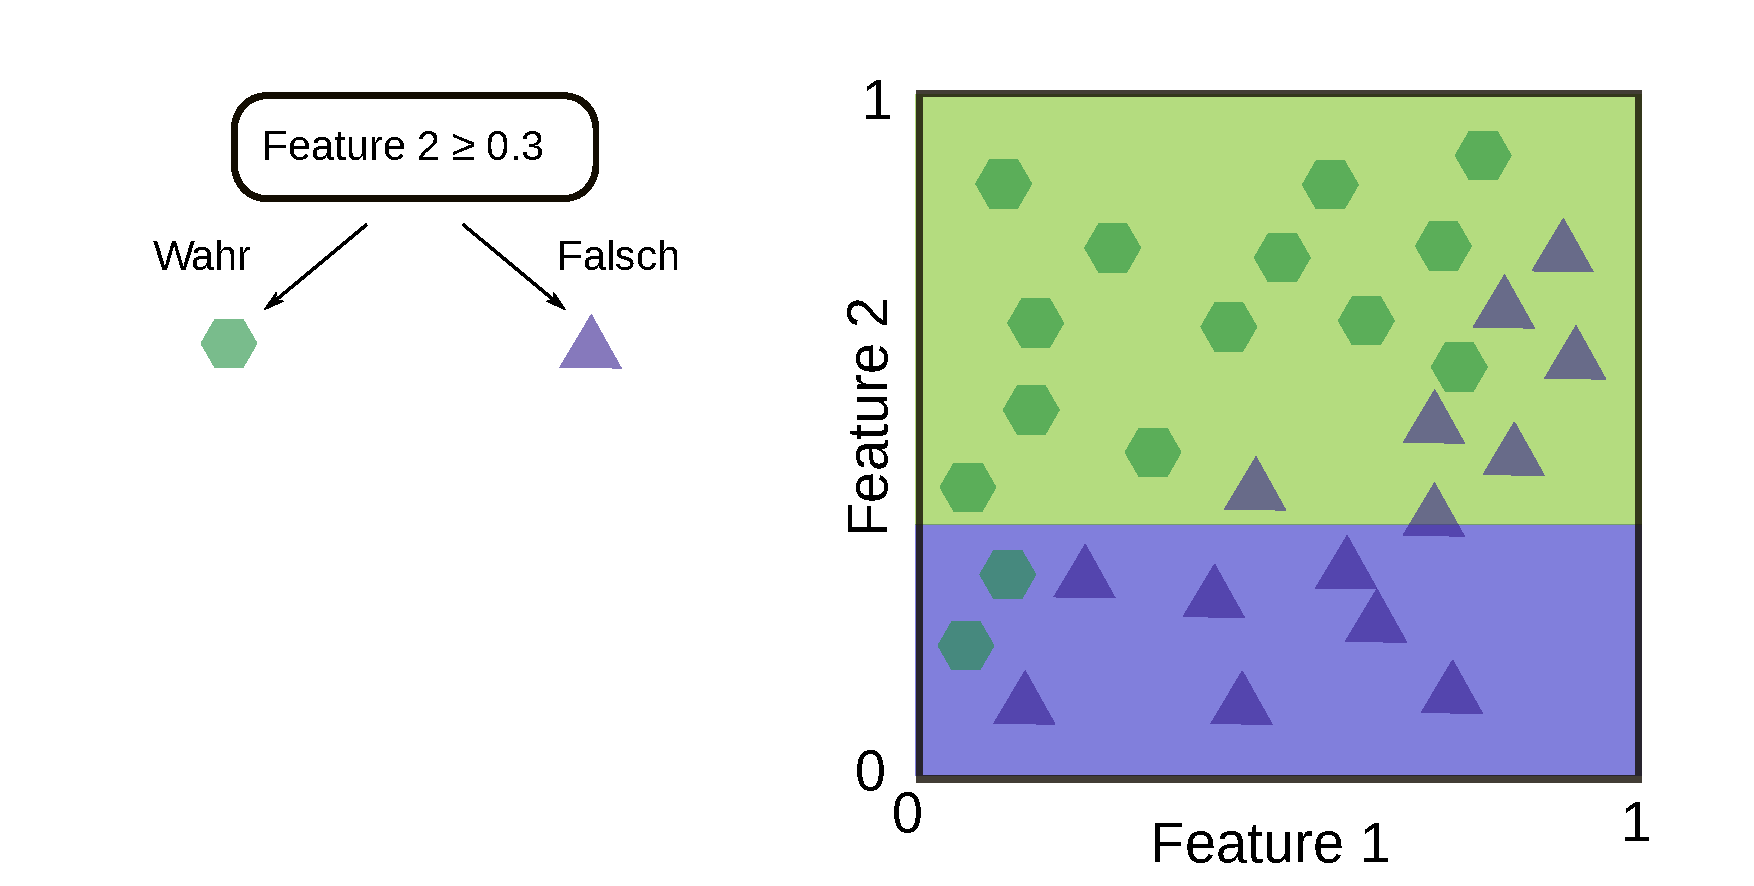
\includegraphics[width=13.0cm]{images/decision_tree_1.pdf}
  \end{center}  
\end{frame}

\begin{frame}
  \frametitle{Entscheidungsbäume (Decision Trees)}
  \begin{center}
    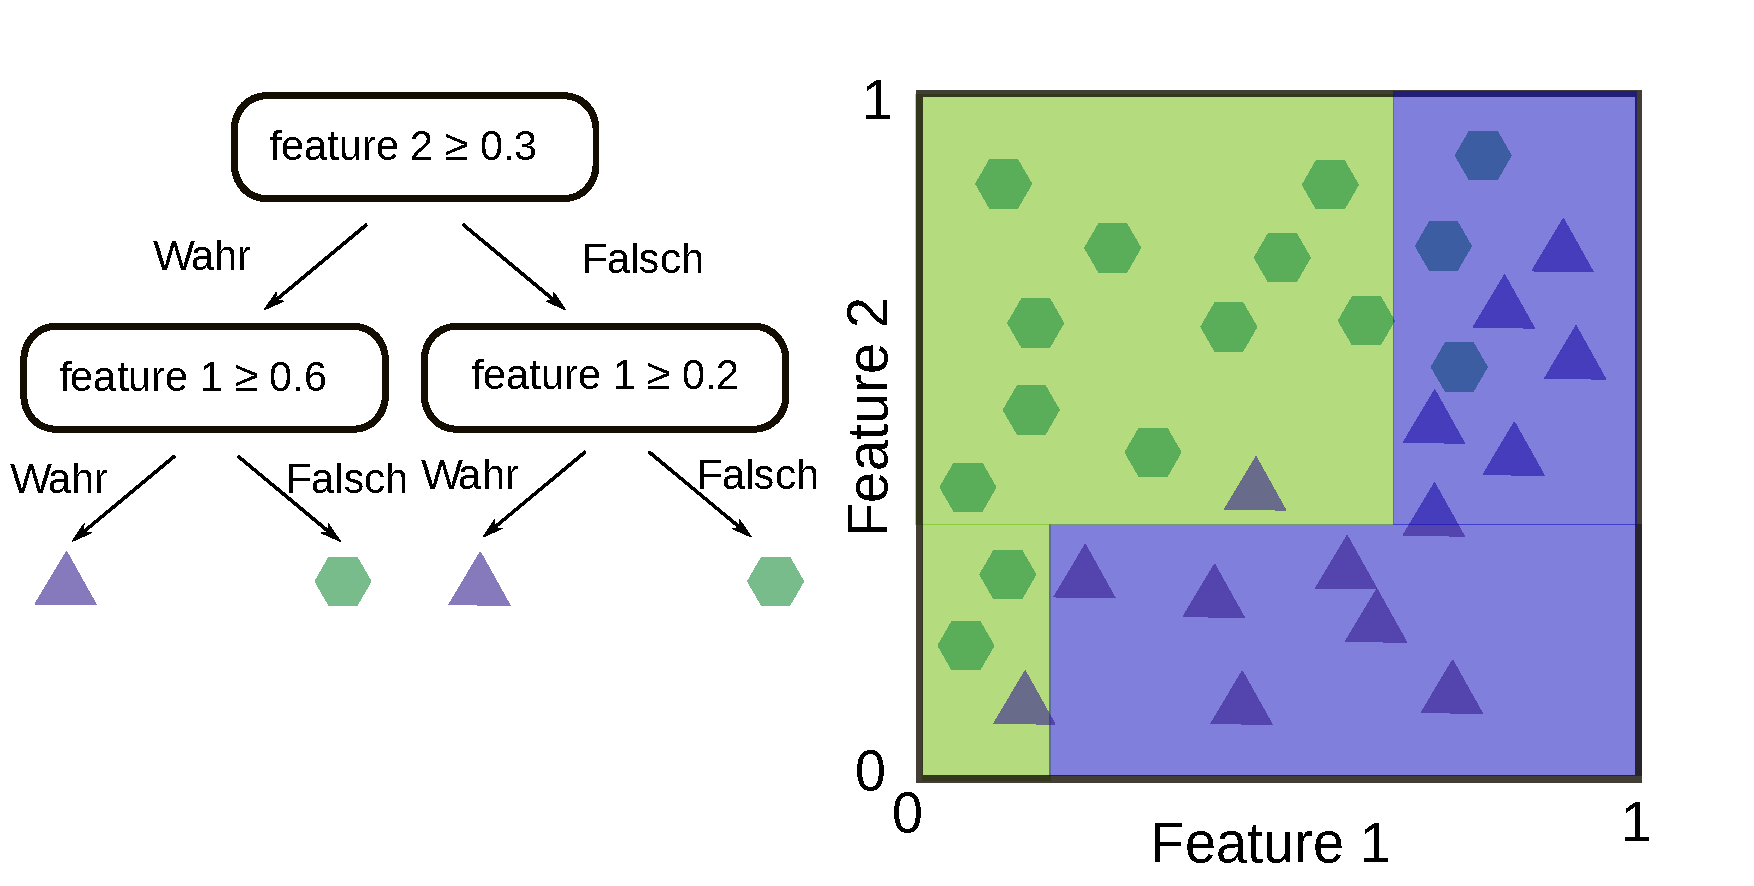
\includegraphics[width=13.0cm]{images/decision_tree_2.pdf}
  \end{center}  
\end{frame}

%% \begin{frame}
%%   Decision trees
%%   \begin{itemize}
%%   \item Concepts:
%%   \item node
%%   \item edge
%%   \item root
%%   \item leaf
%%   \item child
%%   \item parent
%%   \item A forest is a set of n ≥ 0 disjoint trees
%%   \item features: real-valued or categorial and also missing values
%%   \end{itemize}
%% \end{frame}



\begin{frame}
  \frametitle{Entscheidungsbäume (Decision Trees) -- Random Forest}
  \begin{block}{}
    \vspace{0.5cm}
    \begin{minipage}{0.15\textwidth}
      \ \ \
      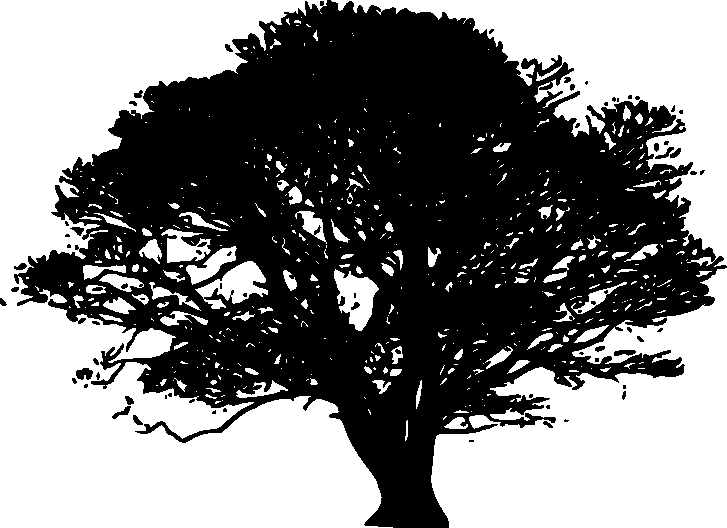
\includegraphics[width=1.6cm]{images/publicdomainvectors_Chrisdesign_Tree_silhouettes_5.pdf}
    \end{minipage}
    \hfill
    \begin{minipage}{0.84\textwidth}
      \begin{itemize}
      \item Einzelne Entscheidungsbäume neigen häufig zum Overfitting.
      \item In der "Random Forest"-Methode werden viele verschiedene
        Entscheidungsbäume zufällig auf verschiedenen Untermengen des
        Trainingsets (einige Entitäten und Attribute) generiert.
      \item Voraussage erfolgt dann über Abstimmung (Voting) der
        Bäume.
      \end{itemize}
    \end{minipage}
    \vspace{0.5cm}
  \end{block}
\end{frame}

%--------------------------------------
\subsection{Künstliche Neuronale Netze}
%--------------------------------------

\setcounter{tocdepth}{2}
\begin{frame}{}
   \tableofcontents[currentsubsection,hideothersubsections,
     subsectionstyle=show/shaded]
\end{frame}


\begin{frame}
  \frametitle{Künstliche Neuronale Netze}
  \begin{block}{}
    \vspace{0.5cm}
    \ \ \ \
    \begin{minipage}{0.05\textwidth}
      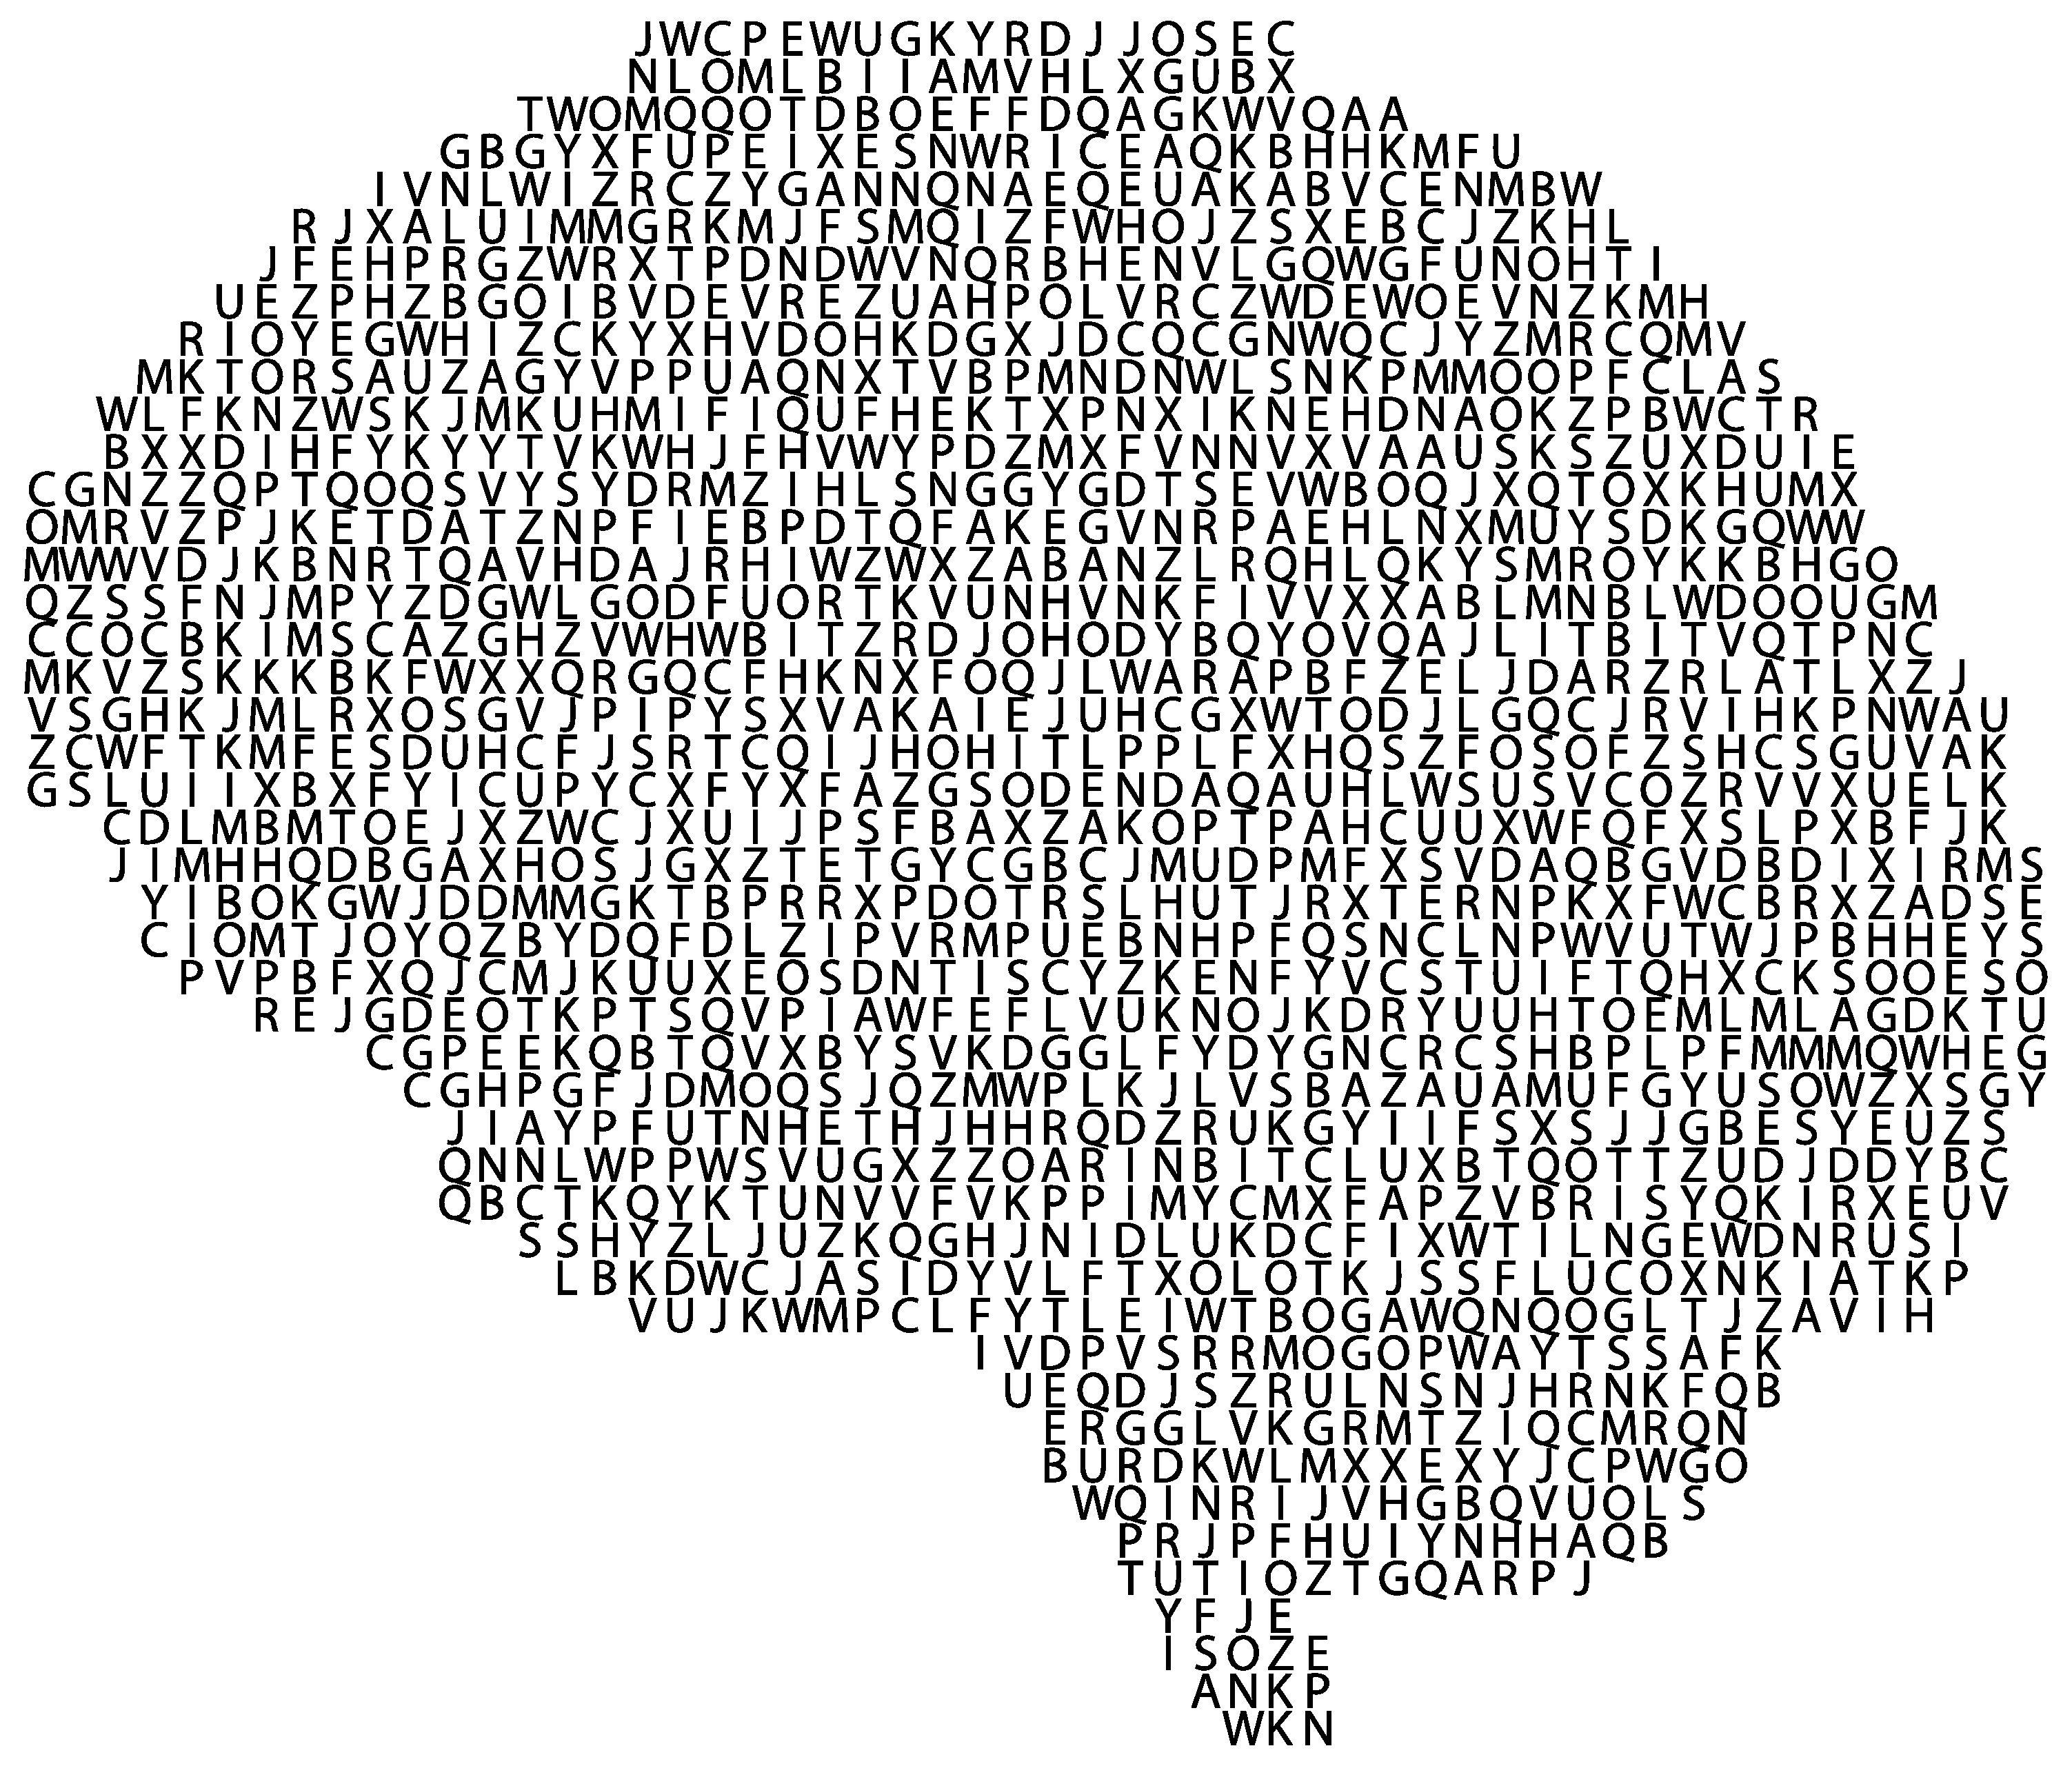
\includegraphics[width=1.6cm]{images/publicdomainvectors_Random-Alphabet-Brain.pdf}
    \end{minipage}
    \hfill
    \begin{minipage}{0.8\textwidth}
      \begin{itemize}
      \item Artificial Neural Networks (ANN), Multilayer Perceptrons
        (MLP) oder Feed-forward Neural Networks
      \item Der Ansatz ist von natürlichen, biologischen neuronalen
        Netzen inspiriert
      \item Kann für Klassifikation und Regression genutzt werden
      \end{itemize}
    \end{minipage}
    \vspace{0.3cm}
  \end{block}
\end{frame}


\begin{frame}
  \frametitle{Künstliche Neuronale Netze}
  \begin{center}    
    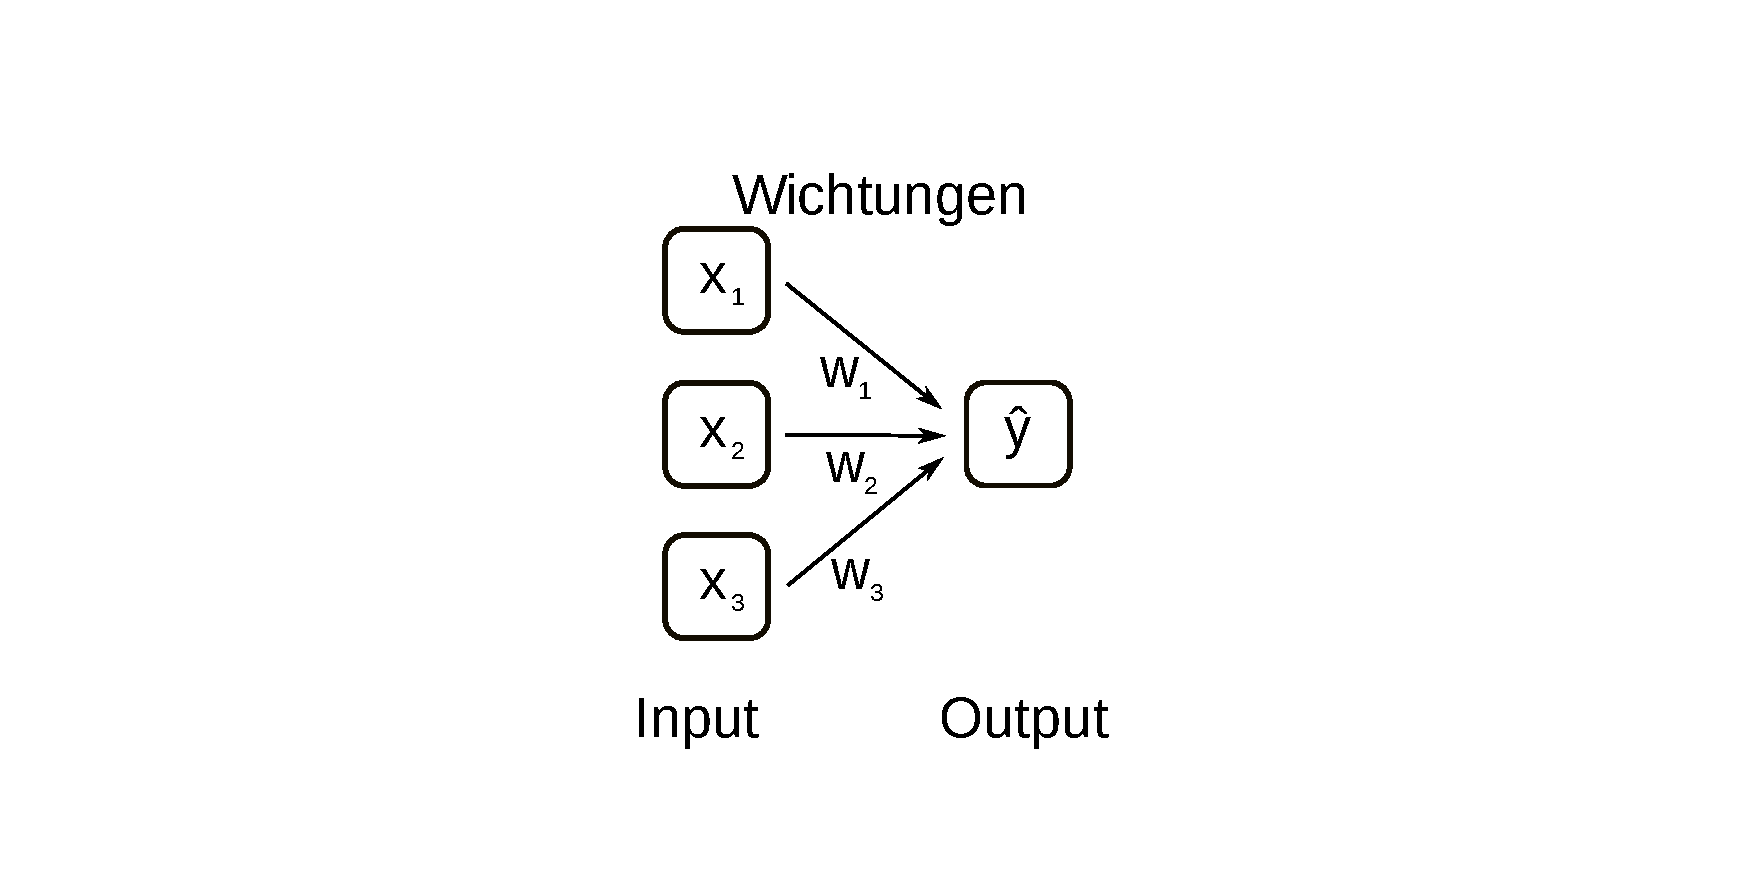
\includegraphics[width=13.0cm]{images/ANN_without_hidden_layer.pdf}
  \end{center}  
\end{frame}

\begin{frame}
  \frametitle{Künstliche Neuronale Netze}
  \begin{center}
    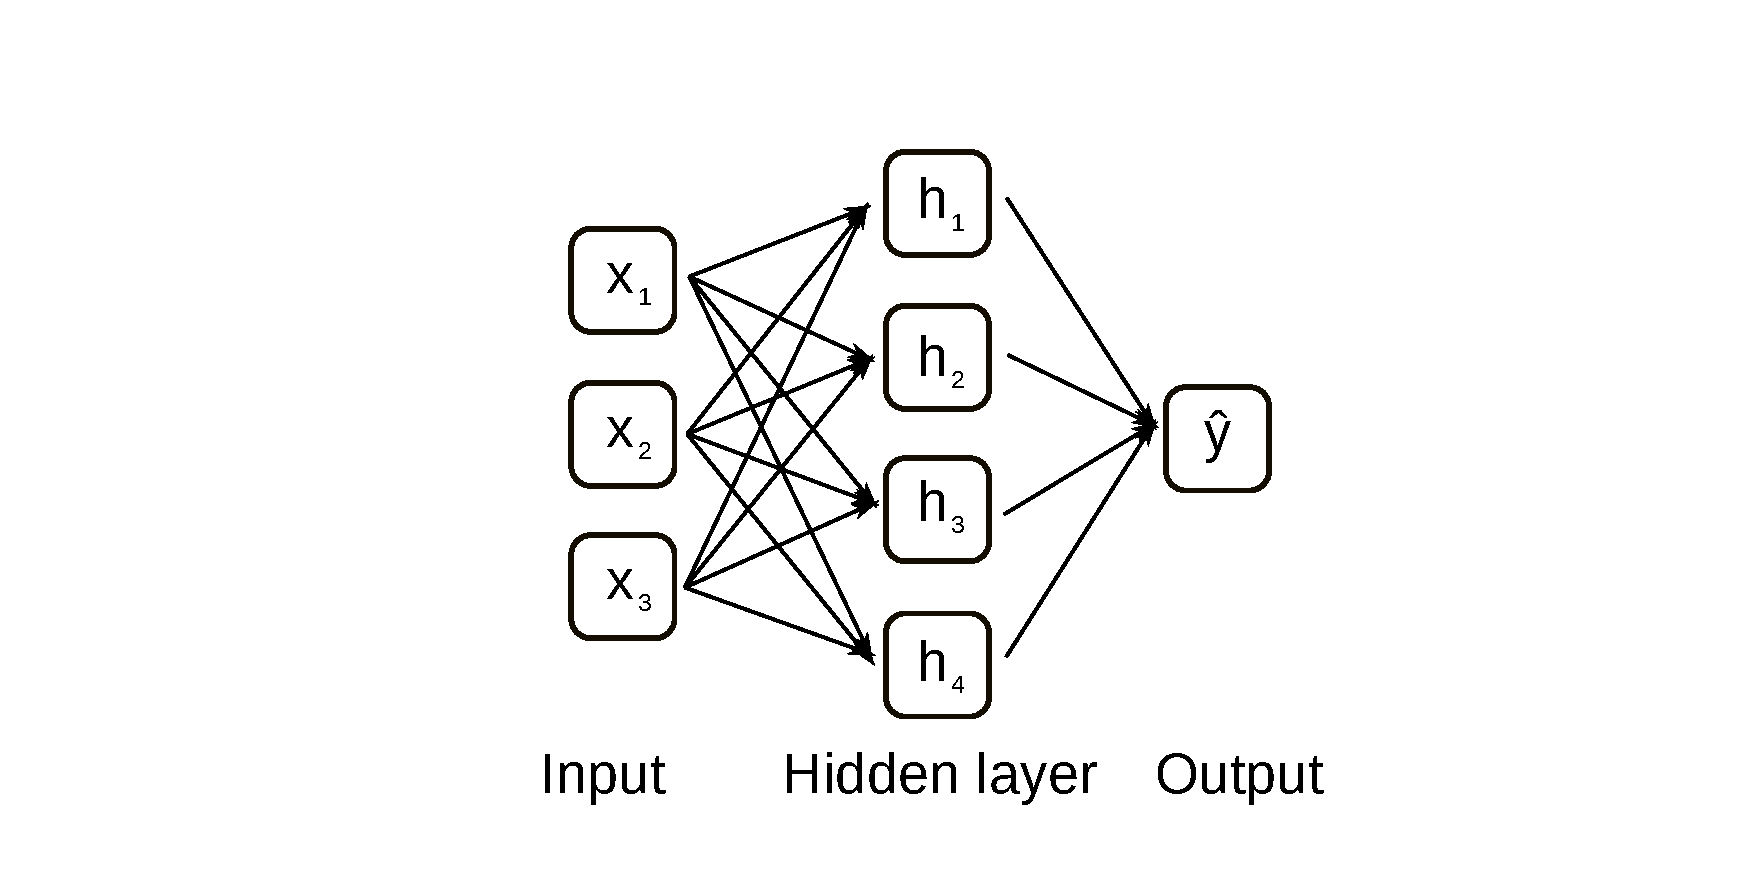
\includegraphics[width=13.0cm]{images/ANN_with_hidden_layer.pdf}
  \end{center}  
\end{frame}


\begin{frame}
  \frametitle{Künstliche Neuronale Netze}
  \begin{center}
    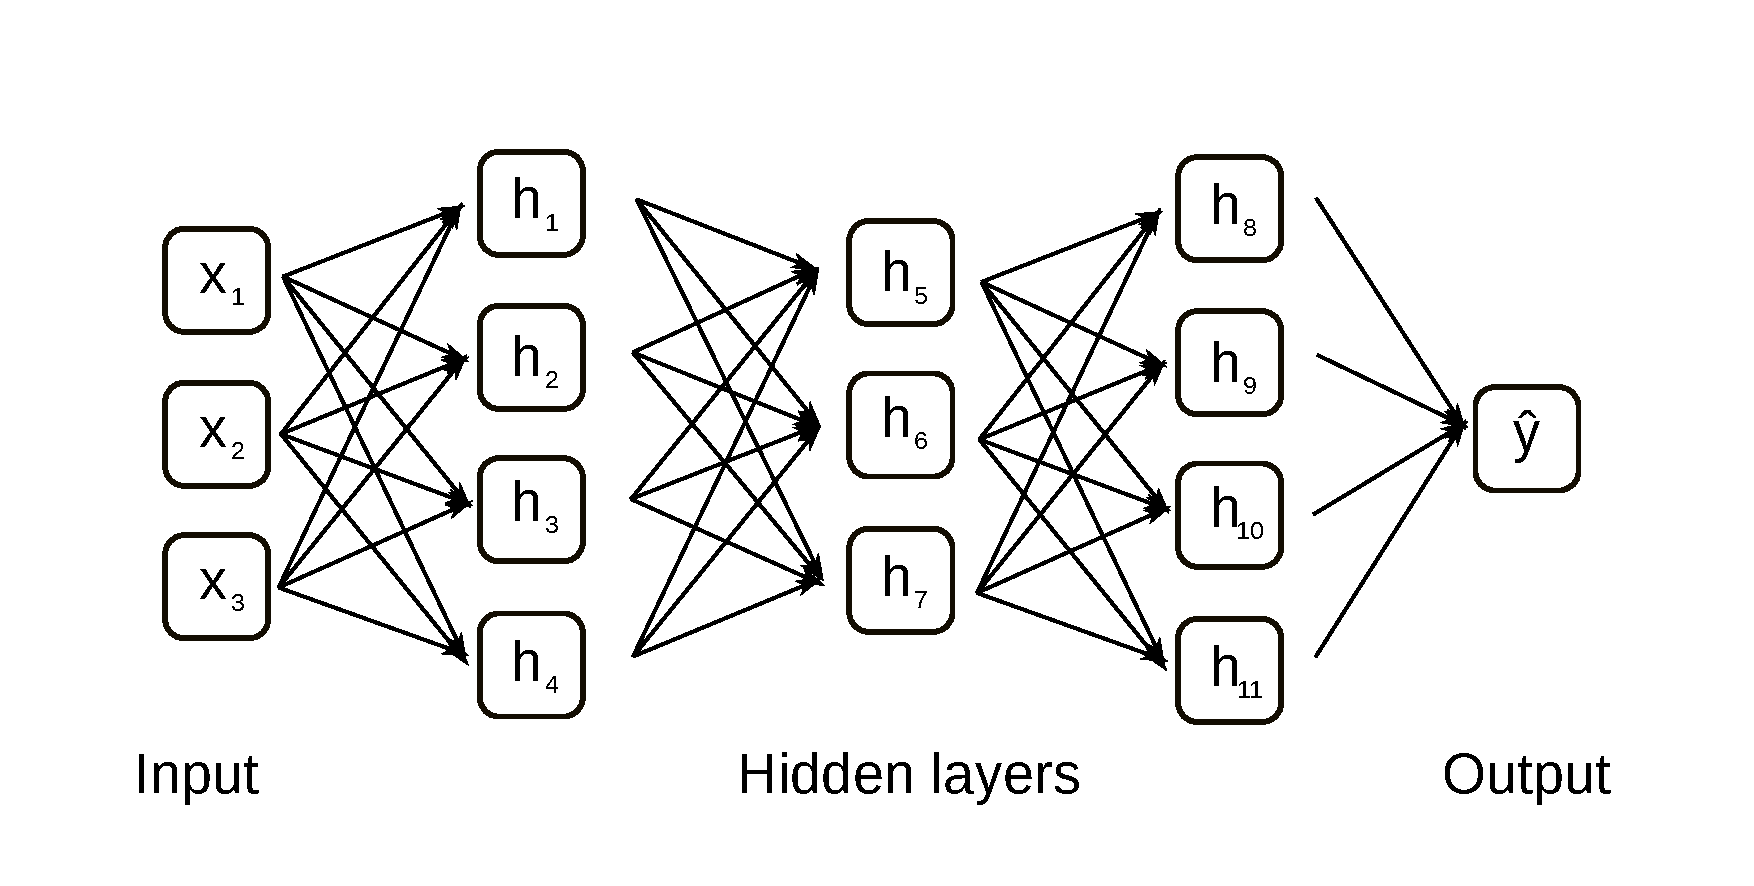
\includegraphics[width=13.0cm]{images/ANN_with_serveral_hidden_layers.pdf}
  \end{center}  
\end{frame}

\begin{frame}
  \frametitle{Künstliche Neuronale Netze -- Deep Learning}
  \begin{block}{}
    \vspace{0.5cm}
    \ \ \ \
    \begin{minipage}{0.05\textwidth}
      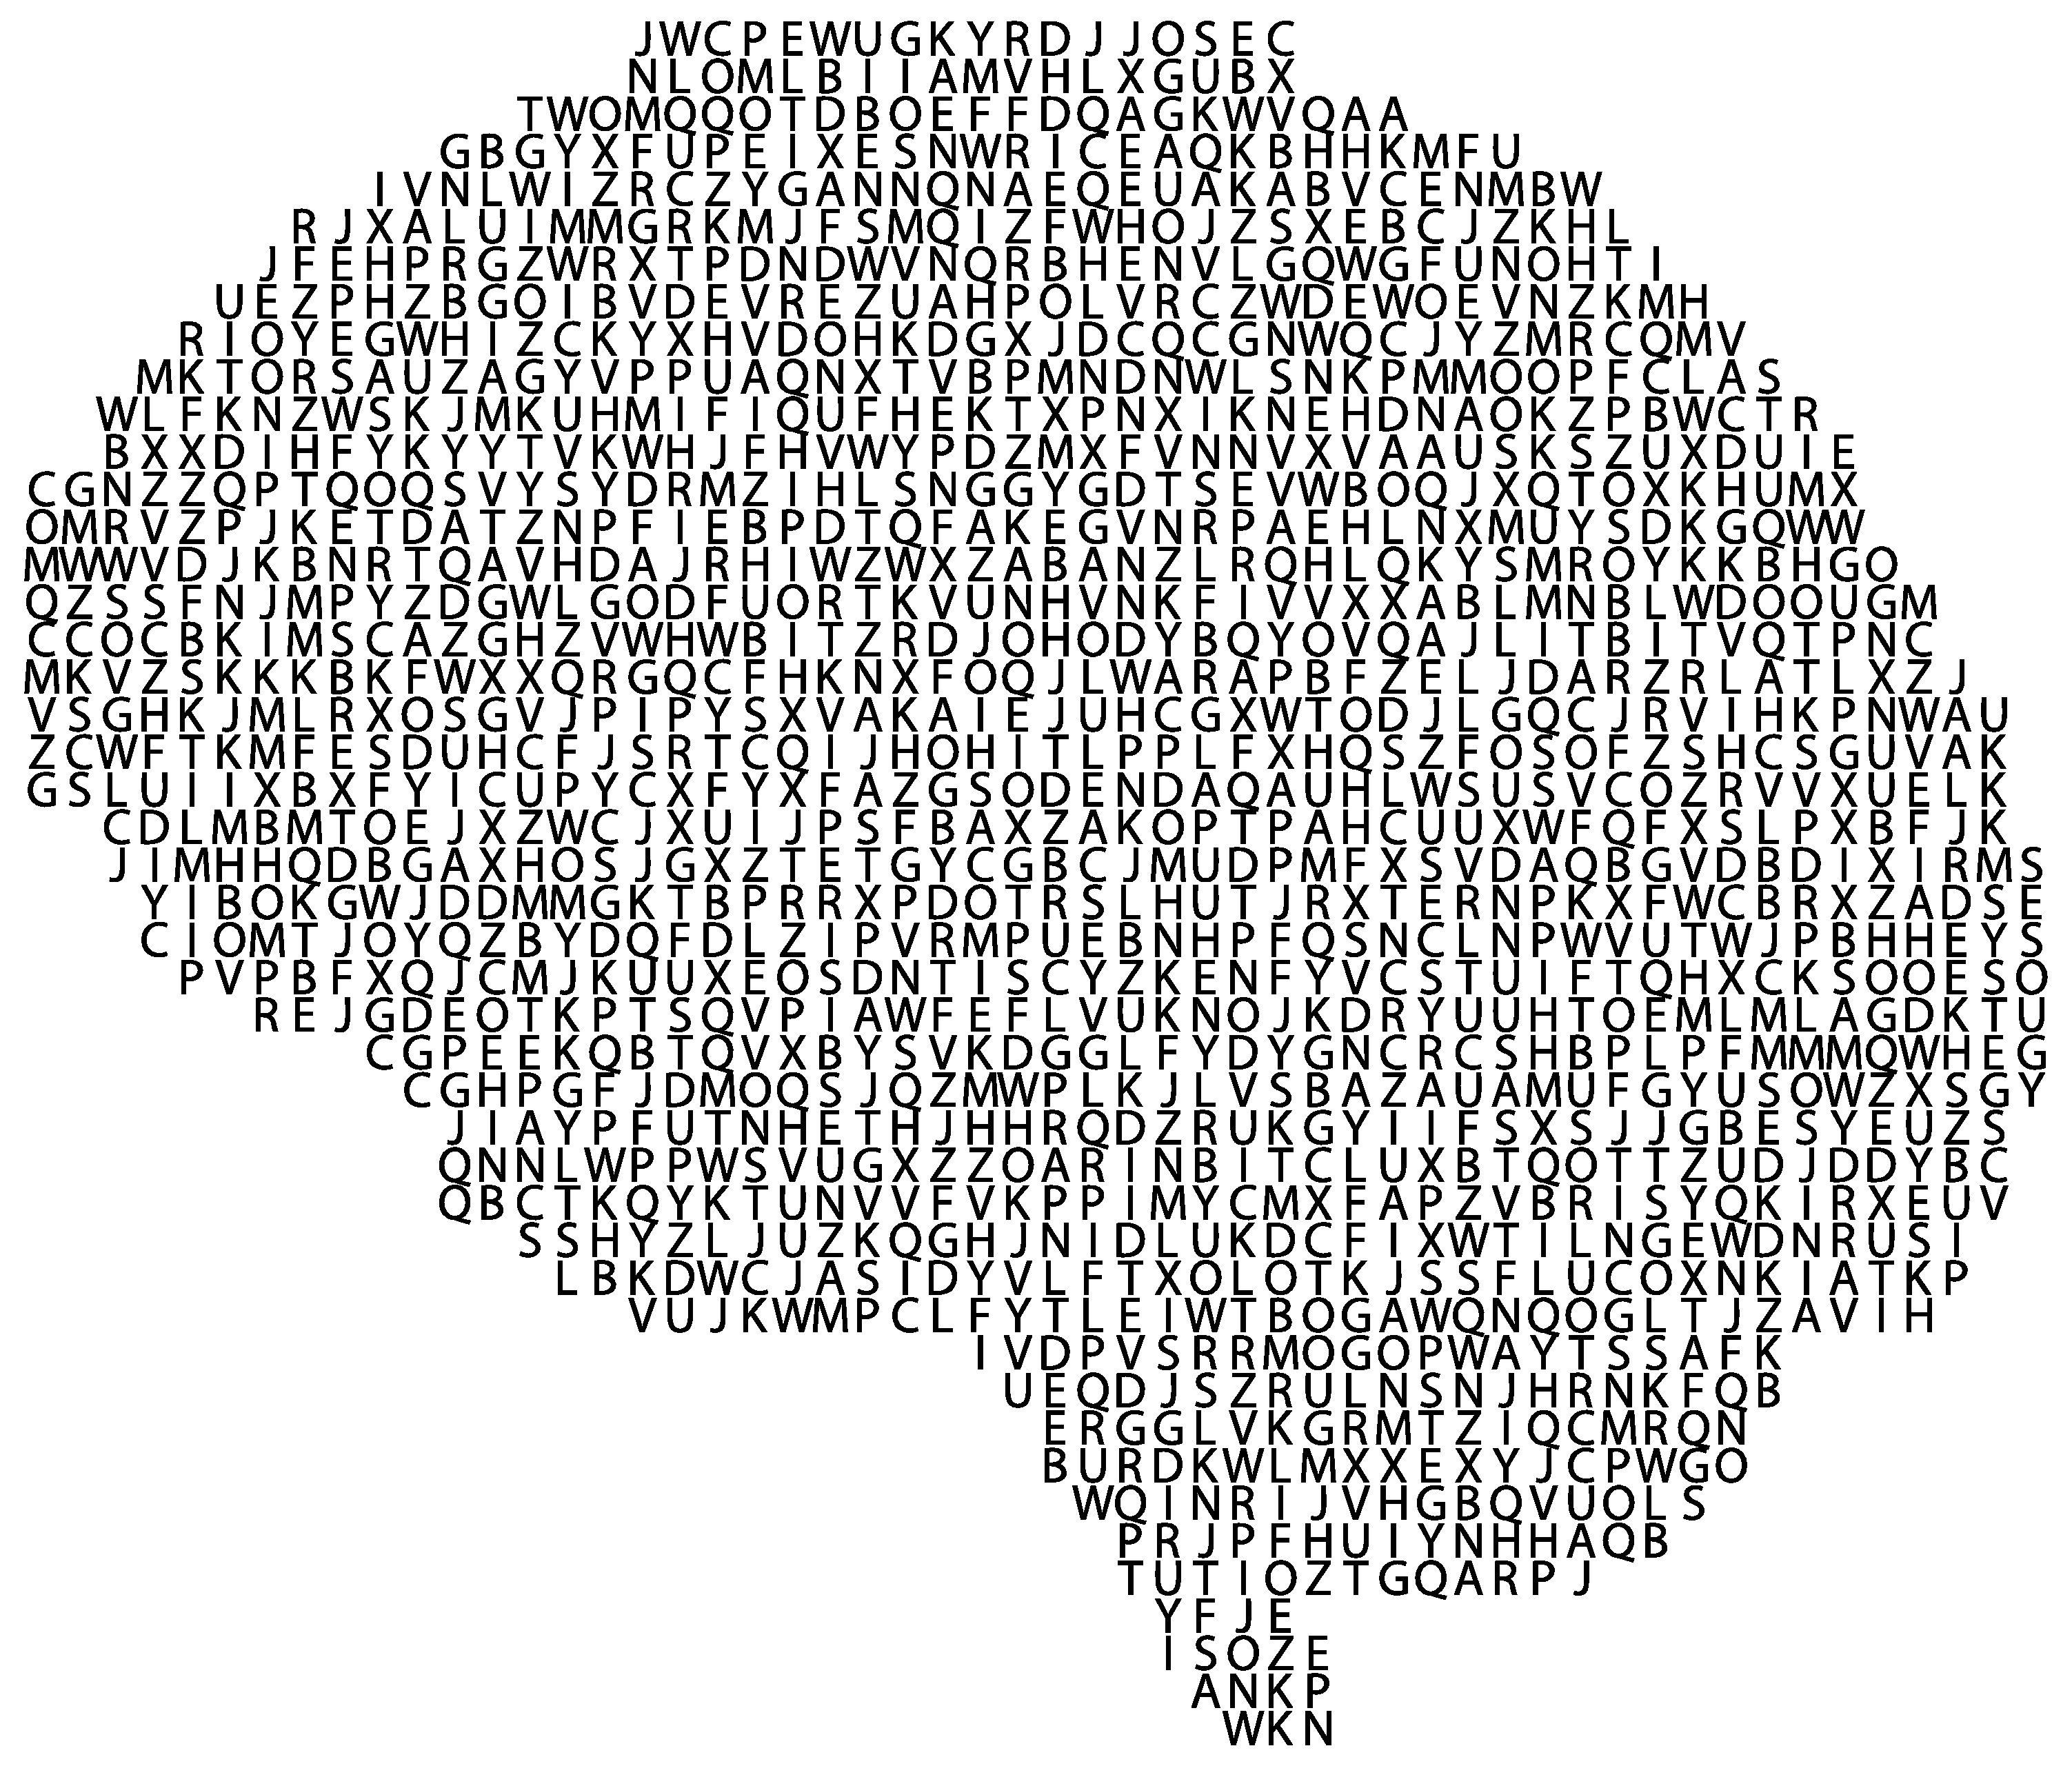
\includegraphics[width=1.6cm]{images/publicdomainvectors_Random-Alphabet-Brain.pdf}
    \end{minipage}
    \hfill
    \begin{minipage}{0.8\textwidth}
      \begin{itemize}
      \item Convolutional Neural Network (CNN) -- u.a. stark in
        Bildanalyse
      \item Recurrent Neural Networks (RNN); Vernetzung von Neuronen
        auch in der derselben Schicht; u.a. stark in der Spracherkennung        
      \end{itemize}
    \end{minipage}
    \vspace{0.3cm}
  \end{block}
\end{frame}


%% \begin{frame}
%%   \frametitle{Artificial Neural Networks}
%%   \begin{center}
%%     ... tomorrow a full session about that 
%%   \end{center}  
%% \end{frame}

%%%%%%%%%%%%%%%%%%%
\section{Unüberwachtes Lernen (Unsupervised Learning)}
%%%%%%%%%%%%%%%%%%%

\setcounter{tocdepth}{1}
\begin{frame}{}
   \tableofcontents[currentsection]
\end{frame}

%%%%%%%%%%%%%%%%%%%%%%%%%%%%%%%%
\subsection{Einführung Unüberwachtes Lernen)}
%%%%%%%%%%%%%%%%%%%%%%%%%%%%%%%

\setcounter{tocdepth}{2}
\begin{frame}{}
   \tableofcontents[currentsubsection,hideothersubsections,
     subsectionstyle=show/shaded]
\end{frame}

\begin{frame}
  \frametitle{Unüberwachtes Lernen -- Anwendungen}
  \begin{block}{}
    \begin{itemize}
    \item Dimesionsreduktion
    \item Clustering
    \end{itemize}
  \end{block}
\end{frame}

%%%%%%%%%%%%%%%%%%%%%%%%%%%%%%%%
\subsection{Dimensionreduktion}
%%%%%%%%%%%%%%%%%%%%%%%%%%%%%%%

\setcounter{tocdepth}{2}
\begin{frame}{}
   \tableofcontents[currentsubsection,hideothersubsections,
     subsectionstyle=show/shaded]
\end{frame}

\begin{frame}
  \frametitle{Dimensionreduktion -- Grundidee}
  \begin{center}
    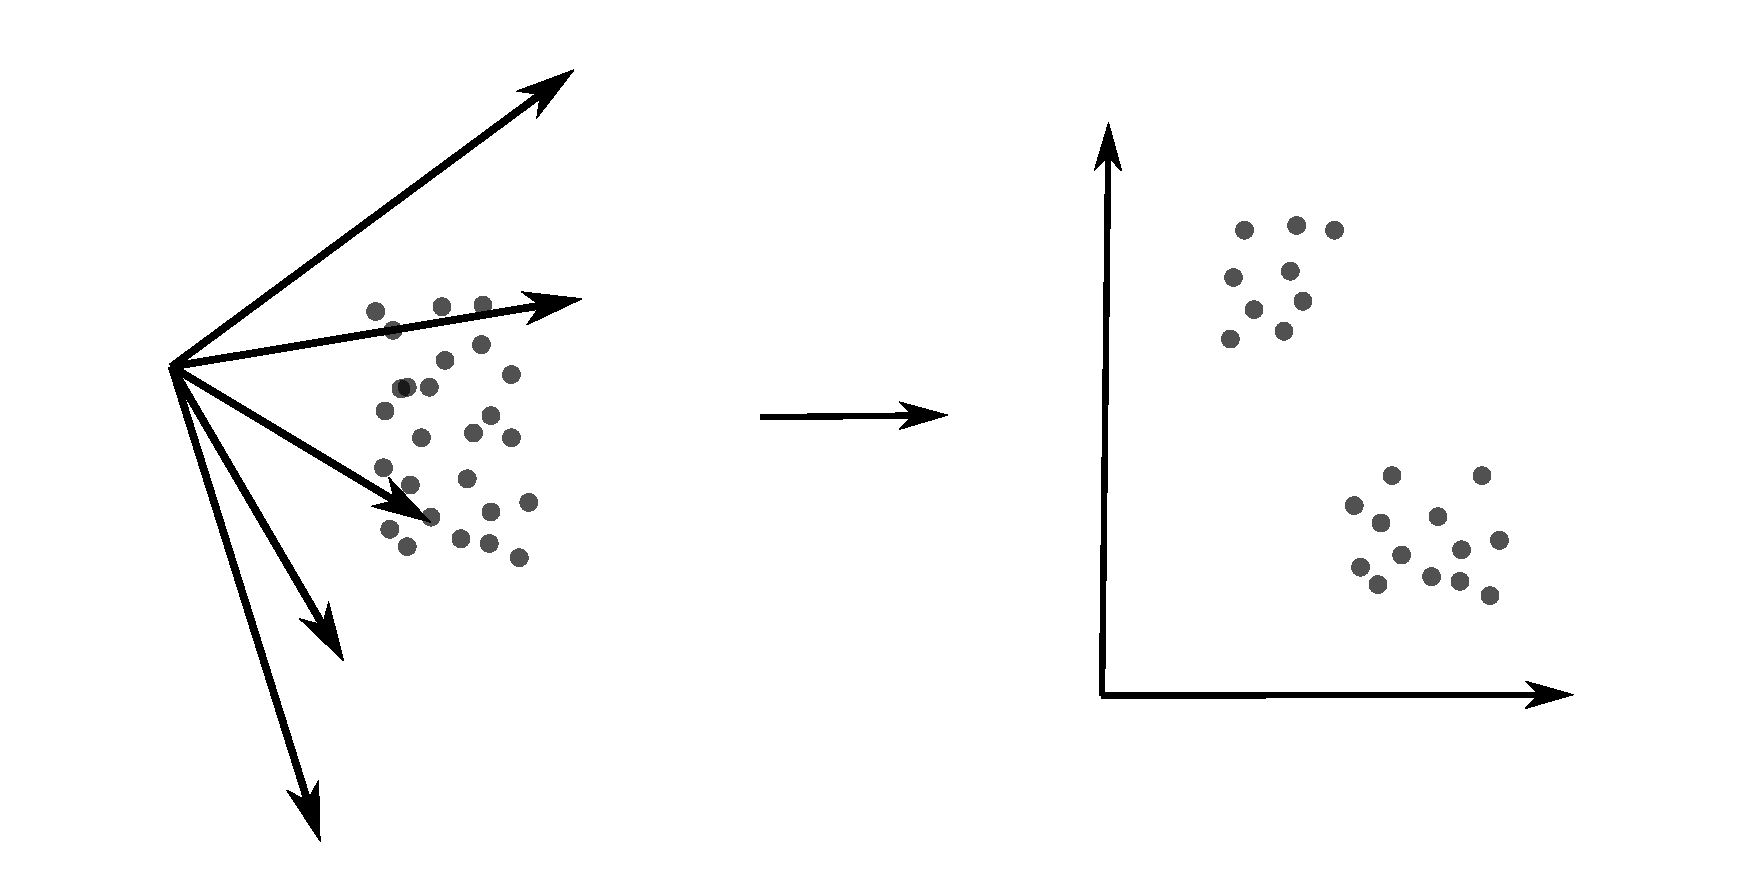
\includegraphics[width=13.0cm]{images/dimension_reduction.pdf}
  \end{center}
\end{frame}

\begin{frame}
  \frametitle{Dimensionreduktion -- Anwendungen}
  \begin{block}{}
    \begin{center}
      \begin{itemize}
      \item Visualisierung
      \item Feature-Auswahl
      \end{itemize}
    \end{center}
  \end{block}
\end{frame}

\begin{frame}
  \frametitle{Dimensionreduktion -- Ausgewählte Methoden}
  \begin{block}{}
    \begin{center}
      \begin{itemize}
      \item Hauptkomponentenanalyse (Principle Component Analysis), lineaer
      \item t-SNE (t-distributed stochastic neighbor embedding), nicht-linear
      \item UMAP (Uniform manifold approximation and projection), nicht-linear
      \end{itemize}
    \end{center}
  \end{block}
\end{frame}

%%%%%%%%%%%%%%%%%%%%%%%%%%%%%%%%
\subsection{Clusteranalysen}
%%%%%%%%%%%%%%%%%%%%%%%%%%%%%%%

\setcounter{tocdepth}{2}
\begin{frame}{}
   \tableofcontents[currentsubsection,hideothersubsections,
     subsectionstyle=show/shaded]
\end{frame}

\begin{frame}
  \frametitle{Clusteranalysen}
  \begin{center}
    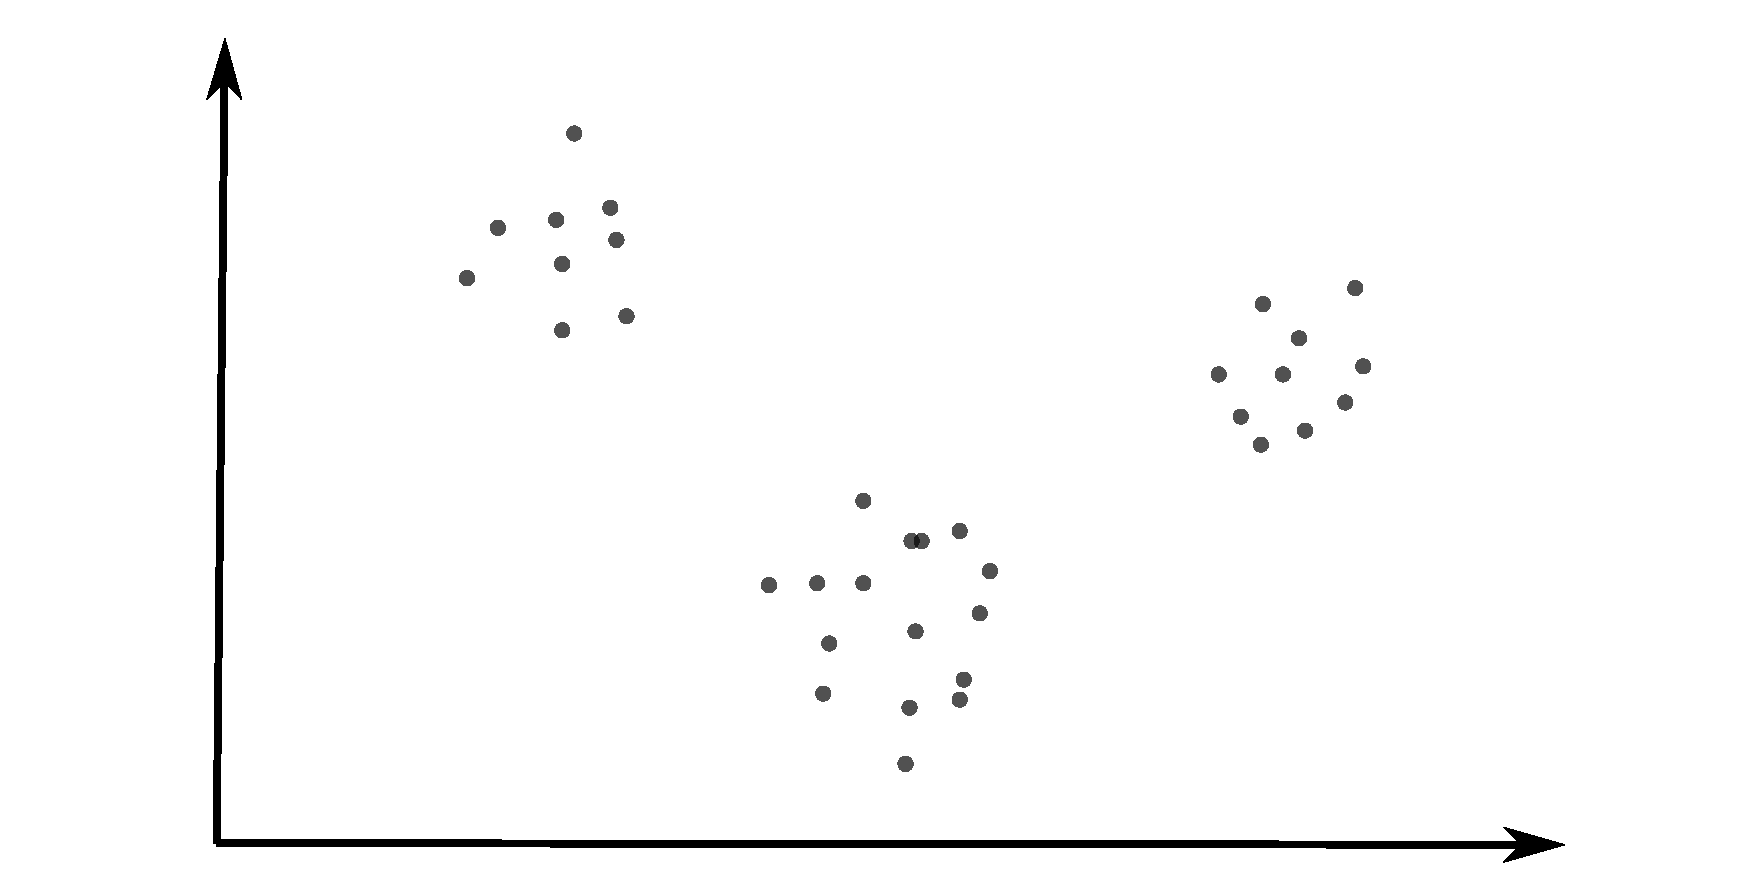
\includegraphics[width=13.0cm]{images/clustering_1.pdf}
  \end{center}  
\end{frame}

\begin{frame}
  \frametitle{Clusteranalysen}
  \begin{center}
    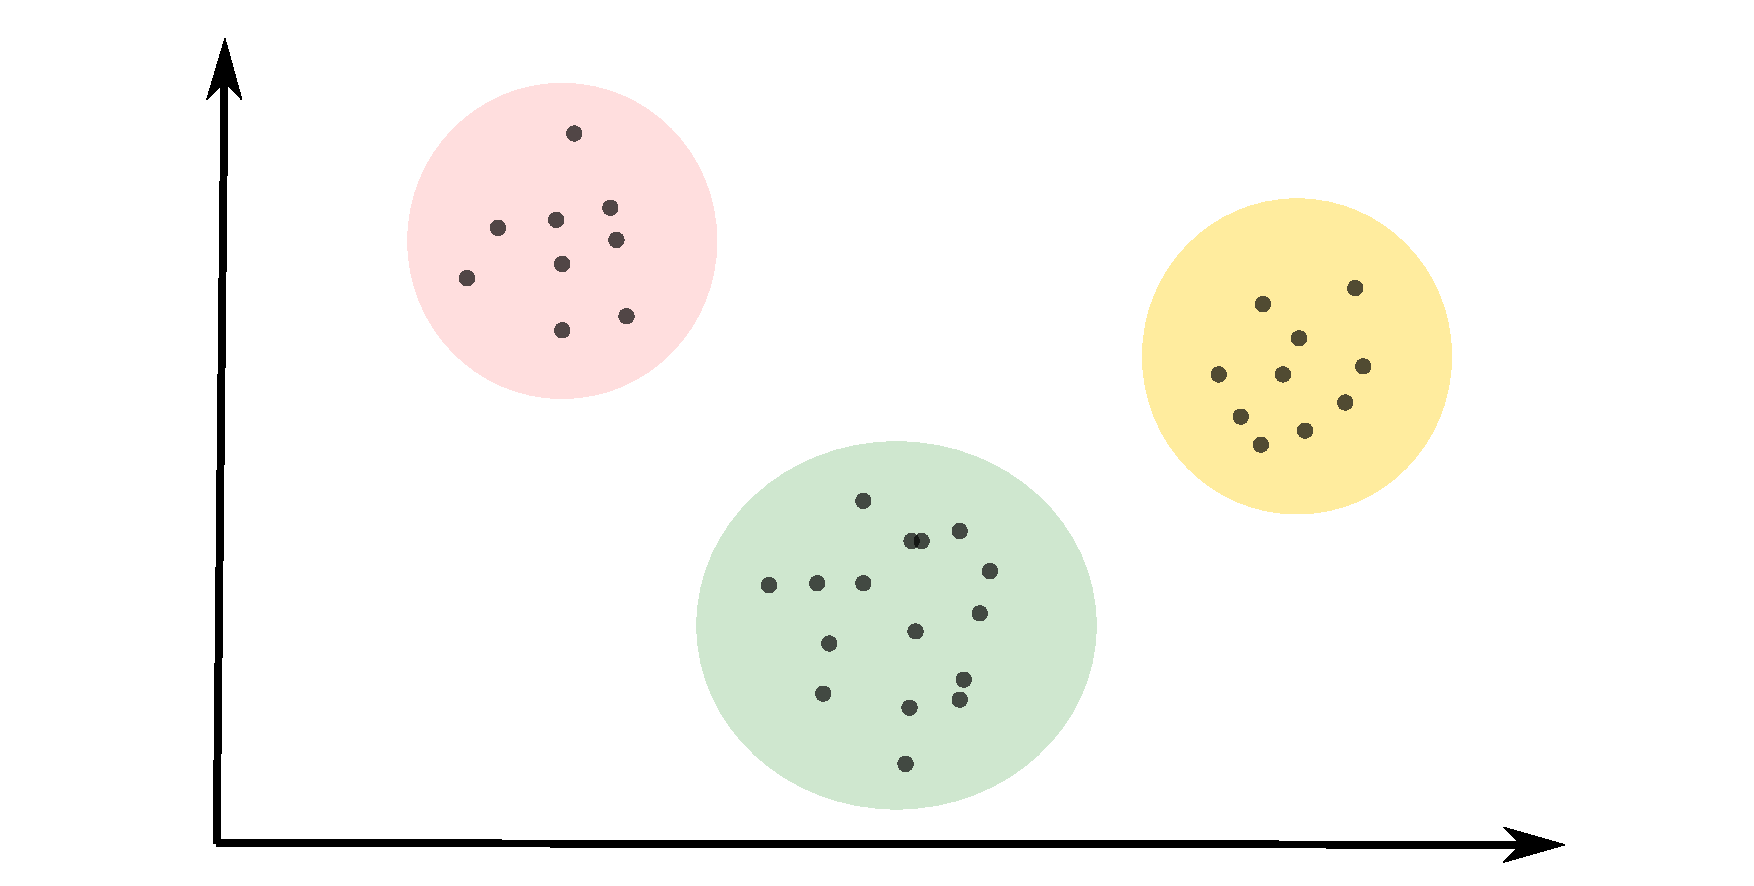
\includegraphics[width=13.0cm]{images/clustering_2.pdf}
  \end{center}  
\end{frame}

\begin{frame}
  \frametitle{Clusteranalysen -- Ausgewählte Methoden}
  \begin{block}{}
    \begin{center}
      \begin{itemize}
      \item k-means Clustering
      \item Hierarchische Clustering
      \item DBSCAN (Density-based spatial clustering of applications
        with noise)
      \end{itemize}
    \end{center}
  \end{block}
\end{frame}

%%%%%%%%%%%%%%%%%%%%
\section{Abschluss}
%%%%%%%%%%%%%%%%%%%%

\begin{frame}{}
   \tableofcontents[currentsection]
\end{frame}

\setbeamertemplate{background}{
  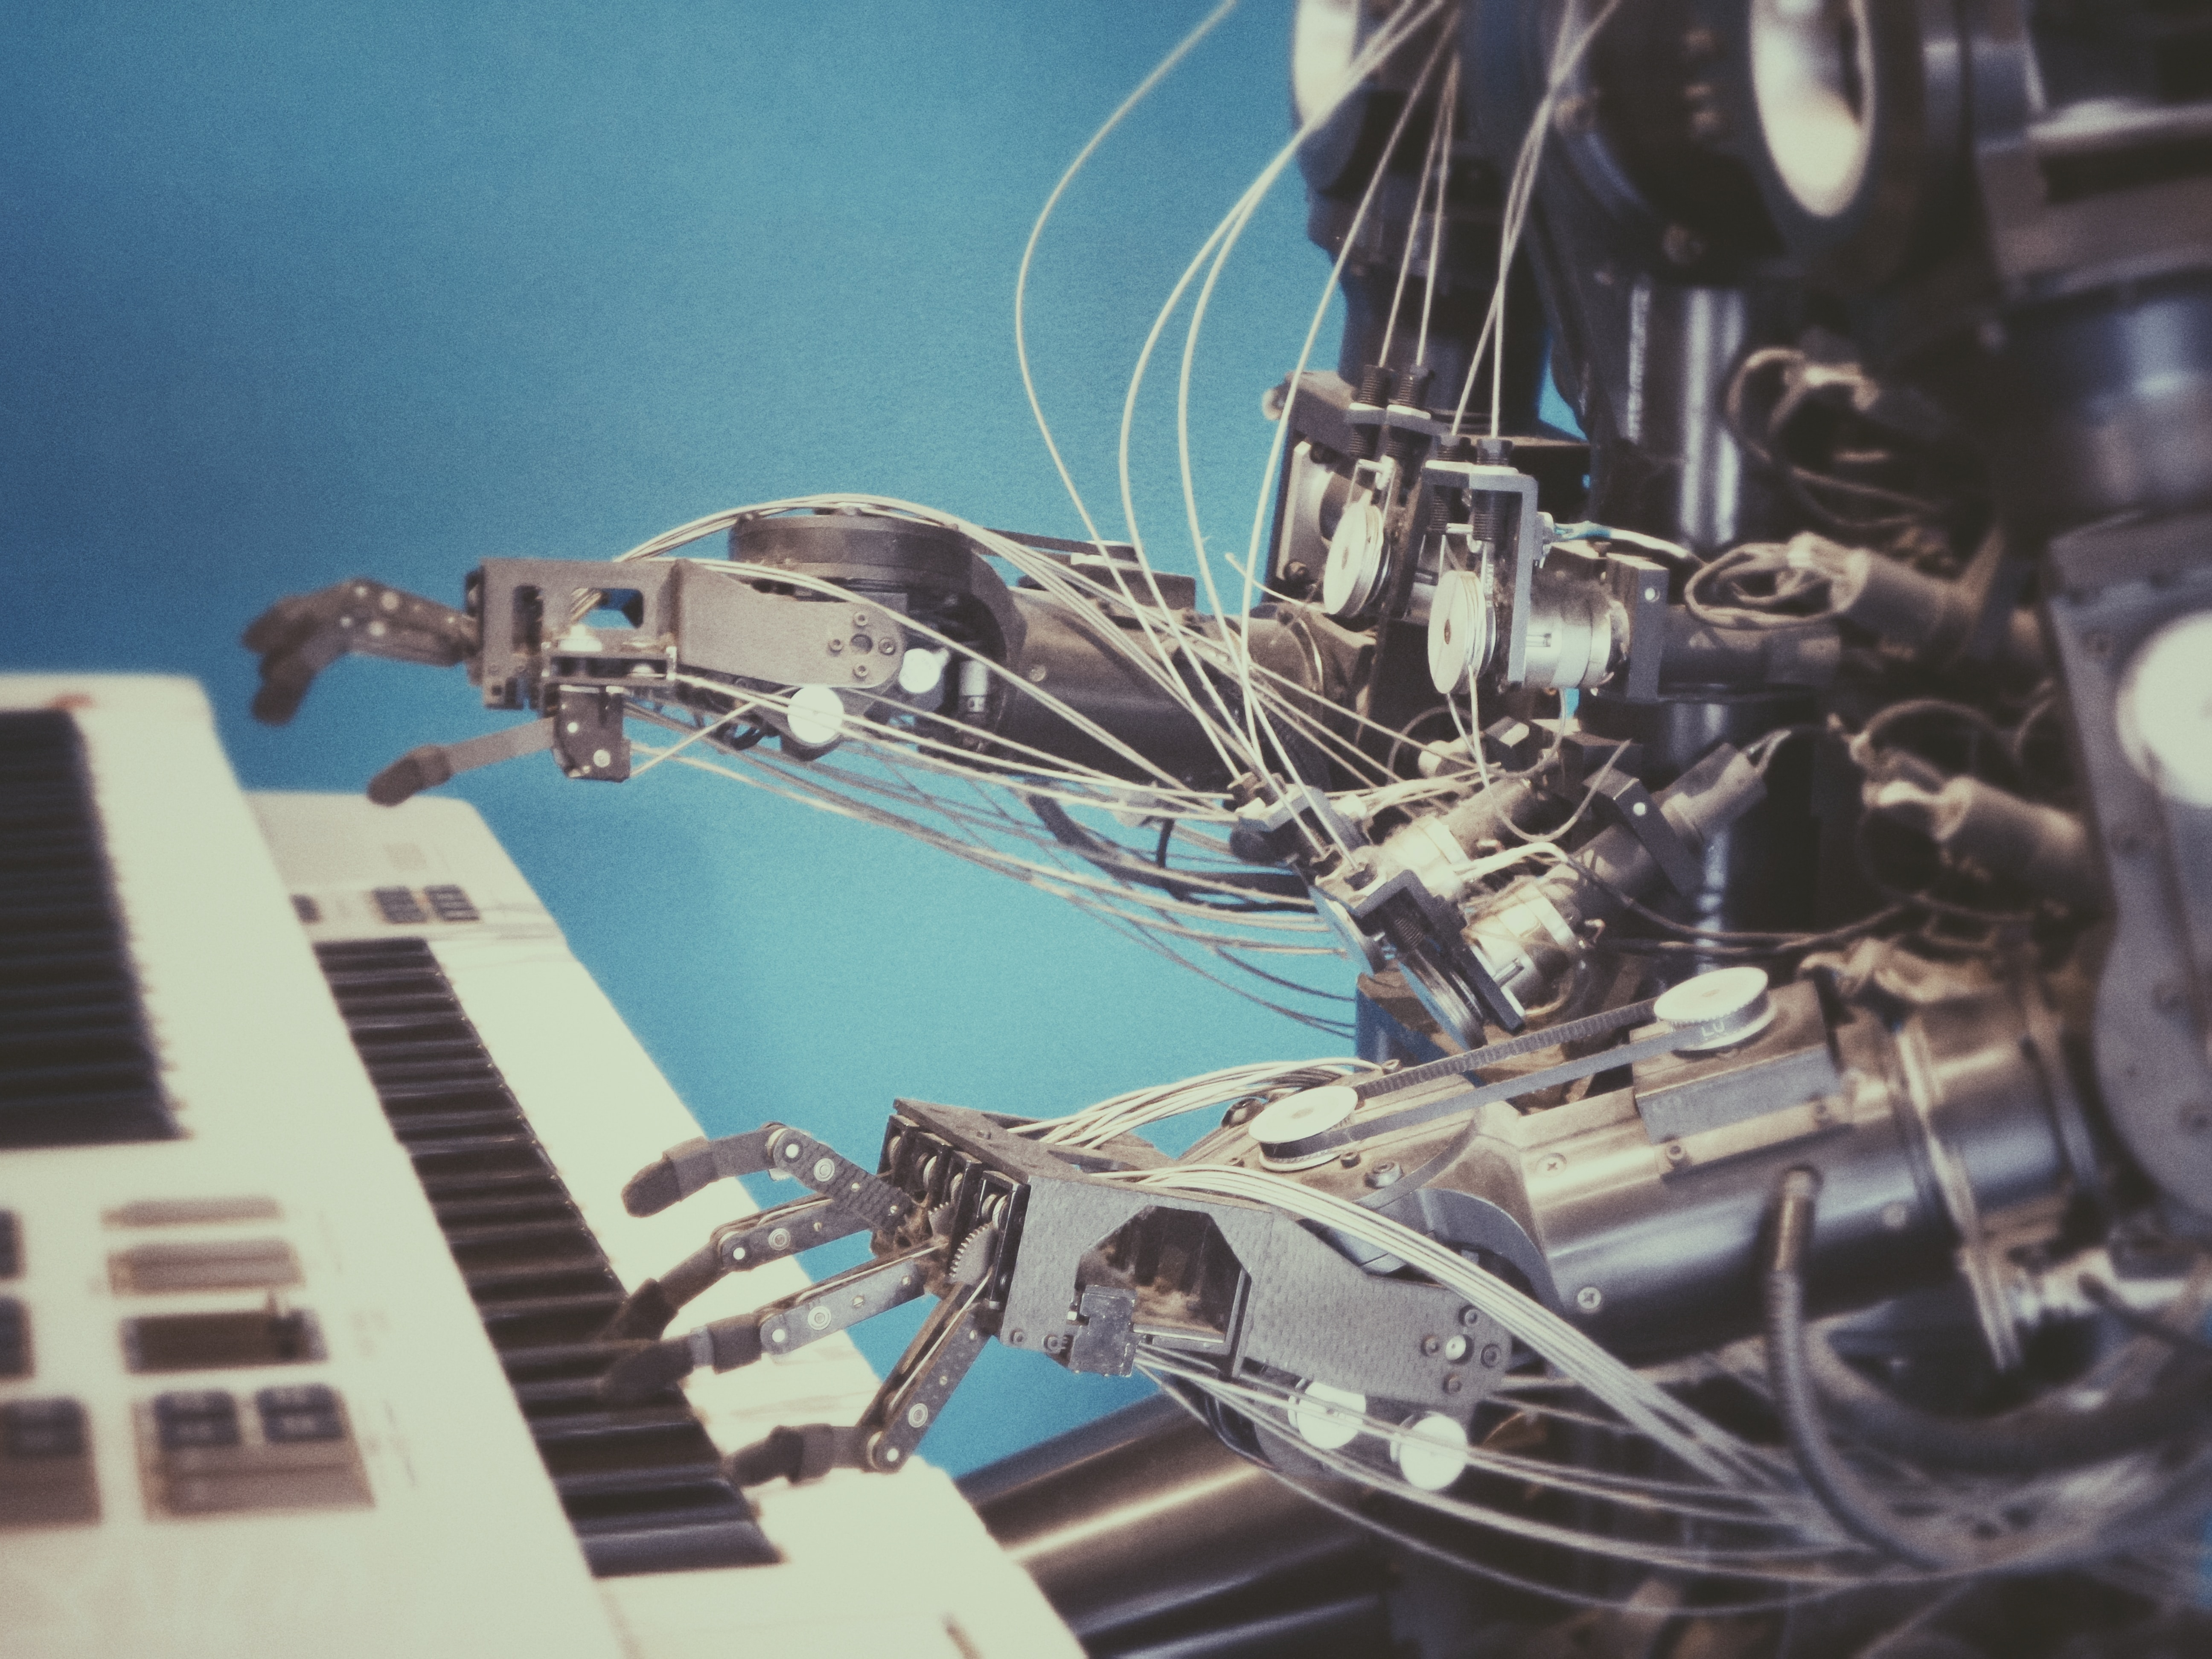
\includegraphics[width=\paperwidth]{images/robot_piano_franck-v-U3sOwViXhkY-unsplash.jpg}}
\setfootercentertext{
  \href{https://unsplash.com/photos/U3sOwViXhkY}{https://unsplash.com/photos/U3sOwViXhkY} -- CC0}
\begin{frame}
  \frametitle{}
\end{frame}
\setbeamertemplate{background}{}
\setfootercentertext{}

\begin{frame}
  \frametitle{Leseempfehlungen}
  \begin{block}{}
    \begin{center}
      \begin{itemize}
      \item Introduction to Machine Learning with Python -- A Guide
        for Data Scientists, Sarah Guido, Andreas Müller, O'Reilly
        Media, 2016, ISBN-13:
        \href{978-1449369415}{https://openlibrary.org/isbn/978-1449369415}
      \item Machine Learning: A Probabilistic Perspective by by Kevin
        P. Murphy, 2012, ISBN-13:
        \href{978-0262018029}{https://openlibrary.org/isbn/9780262018029}
      \end{itemize}
    \end{center}
  \end{block}
\end{frame}

\end{document}
